\documentclass[a4paper,10pt]{article}
\usepackage[toc,page]{appendix}
\usepackage[margin=2.5cm]{geometry}
\usepackage[utf8]{inputenc}
\usepackage{listings}
\usepackage{textcomp}
\usepackage{url}
\usepackage{pdflscape}
\usepackage[nottoc,numbib]{tocbibind}
\usepackage{gnuplot-lua-tikz}
\usepackage{csvsimple}
\usepackage{fancyhdr}
\usepackage{morefloats}
\usepackage[vario]{fancyref}
\usepackage{tikz}
\usepackage{mathtools} 
\usepackage{threeparttable}
\usepackage{subcaption}
\usepackage{placeins}
\bibliographystyle{acm}

\usetikzlibrary{shapes.geometric, arrows, positioning, fit}

\tikzstyle{stepa} = [rectangle, rounded corners, minimum width=3cm, minimum height=1cm, text centered, text width=3cm, draw=black]

\tikzstyle{outcome} = [rectangle, dotted, minimum width=1cm, minimum height=1cm, text centered, text width=3cm, draw=black]

\tikzstyle{infosource} = [circle, minimum width=3cm, minimum height=1cm, text centered, text width=3cm, draw=black]

\tikzstyle{startstop} = [diamond, minimum width=3cm, minimum height=1cm, text centered, draw=black, fill=black!15]

\tikzstyle{phase} = [rectangle, dashed, draw=black]

\tikzstyle{arrow} = [thin,->,>=stealth]

\lstset{upquote=true} 

% Fancyref support for subsections, source; https://github.com/openlilylib/tutorials/blob/master/aGervasoni/orchestralScores/example-materials/OLLbase.sty
\newcommand*{\fancyrefsubseclabelprefix}{subsec}

\fancyrefaddcaptions{english}{%
  \providecommand*{\frefsubsecname}{subsection}%
  \providecommand*{\Frefsubsecname}{Subsection}%
}

\frefformat{plain}{\fancyrefsubseclabelprefix}{\frefsubsecname\fancyrefdefaultspacing#1}
\Frefformat{plain}{\fancyrefsubseclabelprefix}{\Frefsubsecname\fancyrefdefaultspacing#1}

\frefformat{vario}{\fancyrefsubseclabelprefix}{%
  \frefsubsecname\fancyrefdefaultspacing#1#3%
}
\Frefformat{vario}{\fancyrefsubseclabelprefix}{%
  \Frefsubsecname\fancyrefdefaultspacing#1#3%
}
%opening


\title{CITS5502: Assignment 3 -- Modelling the Production of Code}
\author{Ash Tyndall, 20915779}

\begin{document}
\pagestyle{fancy}
\fancyfoot[L]{Ash Tyndall}
\fancyfoot[R]{Assignment 3}
\maketitle
\fontsize{10pt}{11pt}\selectfont
\tableofcontents

\clearpage
\fontsize{11pt}{13pt}\selectfont
\section{Introduction}
If one hopes to predict the time a software development project will take, it is important to be able to understand how to predict the behaviour of code production, or at the very least, know the pitfalls of such predictions. A key part of any such prediction is an investigation of effort and learning. It is readily understood that most processes involving people become more efficient as those people acquire more knowledge about the process; the same could be said of software development. A variety of models have been proposed over the years attempting to model this so called ``learning curve'', such that with sufficient prior data on similar projects, one could make predictions as to how much more efficient a new project with some similarities could be.

There are two different parts to this learning curve; knowledge acquisition and knowledge encoding. Knowledge acquisition deals with general understanding of the problem domain; in the example problems proposed in this unit, they dealt with spherical geometry and various measurements thereof. Knowing generally the equations and algorithms relevant to this mathematical field would be an example of knowledge acquisition.

Knowledge encoding deals with the understanding a person has of the resources they posses to convert the knowledge they have acquired into a software solution that executes a specific task within the problem domain. Knowing the APIs of the given programming language, how to debug it effectively, how to take inputs and outputs as well as the specific syntax to encode the acquired mathematical formula all form part of this knowledge encoding understanding.

Both of these activities are explored within this report within the context of a large data set of solely total programming timings provided from prior CITS8220 course, as well as a smaller data set of personal timings separated into more discrete phases. Using these data sets, several different models of ``learning'' will be explored in terms of how well they appear to operate in real world scenarios, and the parameters these models provide will be analysed to draw conclusions about the nature and effect of prior learning on knowledge acquisition, knowledge encoding, effort estimation, solution consistence and limiting factors. The effectiveness and evolution of my personal software process will also be discussed in this context.

\section{Program Development}
\subsection{Measurement Process \& Data}
The personal data collected for this assignment was collected via a paper worksheet, with the first program being assigned $t=0$, the second $t=1$, etc. This sheet asked the user to note down the ``phase'' of their personal process they were currently in, as well as the minutes they spent in that phase. This paper was next to each participant as they researched and wrote their solution. This type of data recording was adequate, however, there were inaccuracies introduced into the collection by the phases not being immediately recorded on the sheet when they were exited. Participants would also become distracted by their research or development, and switch phases quickly several times, and these phases were only recorded some minutes after they had occurred. This has a potential to introduce inaccuracies.

Also, in some cases the phases the participants had defined in their processes were being iterated through too fast to readily note on the paper worksheets. For instance, in my personal process, there is a phase for both the testing of the solution and the fixing of found bugs. Generally, a test phase would last mere seconds, as it involved running the program and comparing its output, and the resulting fix phase would also be very quick as the errors were normally quite apparent. This test and fix phase would be alternated between many times in the space of minutes. This behaviour is difficult to record accurately on a paper worksheet. 

An alternate way of measuring this software development would be to utilise screen recording software on the development machine, then record the amount of time spend in each phase after the fact. This would prevent the overhead of the paper worksheet, as participants would not have to ensure they are noting their phases down at that time. It would also lead to a more organic definition of the phases, as it was discovered that my personal process as defined did not map to my personal process in practice (further discussion in \fref{subsec:personalprocesseval}).

\subsection{Issues}
In terms of the software development itself, overall there were few issues with the implementation of the programs themselves, with the exception of $t=2$. With $t=2$, I was asked to develop a program that could calculate the area of a quadrilateral given four points on the Earth's surface. I had forgotten at this point that in the prior program we had used a simple non-right-angle triangle area formula in combination with great circle distance calculations to calculate the area of a given three points on the Earth's surface. Due to this, much time was lost researching the calculation of the area of a spherical triangle using spherical geometric methods, which proved to be difficult to understand and implement without prior understanding of them. Ultimately, the time this program took was completely blown out, and serves as an extreme outlier within my personal development data set.

To counteract this, the quadrilateral area program was redeveloped again blind as $t=3$, and data analysis within this assignment is performed with either the outlier included and excluded (see individual captions for clarification) to account for the effect this has on the data set where appropriate. 


\section{Effort Models}
\begin{table}
  \centering
  \begin{threeparttable}
  \begin{tabular}{|c|rrrr|rrrr|rrrr|}
  \hline
 & \multicolumn{4}{|c|}{Problem 1 Language A} & \multicolumn{4}{|c|}{Problem 2 Language A} & \multicolumn{4}{|c|}{Problem 1 Language B} \\
$t$ & 0 & 1 & 2 & 3 & 0 & 1 & 2 & 3 & 0 & 1 & 2 & 3 \\ \hline
P1 & 270 & 170 & 117 & 114 & 50 & 61 & 45 & 40 & 105 & 80 & 60 & 60 \\
P2 & 55 & 20 & 19 & 18 & 83 & 14 & 13 & 13 & 115 & 35 & 29 & 41 \\
P3 & 205 & 165 & 58 & 64 & 150 & 115 & 107 & 102 & 159 & 113 & 87 & 83 \\
P4 & 169 & 82 & 47 & 27 & 73 & 38 & 91 & 59 & 106 & 22 & 28 & 28 \\
P5 & 150 & 75 & 63 & 45 & 75 & 79 & 27 & 26 & 73 & 135 & 28 & 66 \\ \hline
$\mu$ & 169.8 & 102.4 & 60.8 & 53.6 & 86.2 & 61.4 & 56.6 & 48.0 & 111.6 & 77.0 & 46.4 & 55.6 \\ \hline
  \end{tabular}
  \begin{tablenotes}
      \item $\mu$: Mean
  \end{tablenotes}
  \caption{CITS8220 raw data}
  \label{tab:rawdata}
  \end{threeparttable}
\end{table}
Four separate models for effort were proposed, each of which models effort (in minutes, for our situation) on a different curve. These curves all share the same constants, $a$, $b$, and $c$, which represent different parts of the effort modelled, as well as the factor $t$ representing time progression.

\begin{equation} \label{eq:1}
\textit{Effort} = \frac{a+bct}{bt+1}\tag{A}
\end{equation}

\begin{equation} \label{eq:2}
\textit{Effort} = (a-c)(t+1)^{-b}+c\tag{B}
\end{equation}

\begin{equation} \label{eq:3}
\textit{Effort} = (a-c) \mathrm{e}^{-bt} +c\tag{C}
\end{equation}

\begin{equation} \label{eq:4}
\textit{Effort} = a+bt+ct^2\tag{D}
\end{equation}

Each model has a slightly different curve to represent the combination of factors;

\begin{itemize}
 \item Model A represents these factors in terms of the positive part of a hyperbolic equation. This equation is based upon the work of John Musser, among others.
 \item Model B also represents these factors in terms of a hyperbolic equation, however, in this version the effect of $b$ is more highly emphasised. This equation has its roots in psychological Learning Theory.
 \item Model C represents these factors in terms of the basic exponential equation $y = a \mathrm{e}^{bx}$, with modifications to be negatively exponential and include the $c$ parameter.
 \item Model D represents these factors in terms of a general quadratic parabolic equation.
\end{itemize}

\subsection{Model Suitability}
To suitably model a ``learning curve'', a model must meet certain criteria. Some primary criteria the model must cater for include;
\begin{itemize}
 \item The model must show reduced effort over time, as knowledge acquisition over time results in reduced effort.
 \item The model must reflect that all tasks have a non-zero ``minimum effort'' required to complete them, regardless of level of knowledge (parameter $c$).
 \item The model must reflect that initial knowledge about a task affects the initial effort of the task on the curve at $t=0$ (parameter $a$).
 \item The model must reflect that different people learn at different rates, therefore the curve's rate of decrease differs from person to person (parameter $b$).
\end{itemize}

Models A, B and C reflect these parameters well. All three of these models show the effort reduction $f(t+1) < f(t)$ for $t > 0$, and they include the relevant parameters $a$, $b$, and $c$ to allow both the fixed effort, the initial effort and the learning curve to be appropriately modelled.

However, model D does not meet $f(t+1) < f(t)$ for $t > 0$, as it is parabolic in nature. Due to this, this model will actually reflect \textit{increased} effort as $t$ rises beyond a certain point. This makes the model wholly unsuited for modelling effort, as such an increase of effort is not consistent with knowledge acquisition principles.

\subsection{Best Fitting Model}
Five people from the supplied CITS8220 data were chosen randomly and relabelled as persons P1--P5. For each of the three problem sets on which data exists (Problem 1 Language A, Problem 2 Language A, and Problem 1 Language B) the four datapoints of each of the five persons were averaged to produce 3 sets of four points (see \fref{tab:rawdata}).

These points were fitted to all models,\footnote{While assignment directions specified choosing 2 models, it was no more effort to fit against all 4.} using a non-linear least-squares regression method in Matlab (see appendix \fref{sec:graphgencode}). Each of these graphs (see appendix \fref{sec:cits8220results}) produced an $R^2$ value indicating the quality of the fit.\footnote{Traditionally, $R^2$ values are not negative. To quote the Matlab documentation; ``Note that it is possible to get a negative R-square for equations that do not contain a constant term. Because R-square is defined as the proportion of variance explained by the fit, if the fit is actually worse than just fitting a horizontal line then R-square is negative.'' For our purposes, to avoid affecting averages, any $R^2$ value that is negative has been set to 0, indicating no fit.} \Fref{tab:avgr2} shows these results for each person and model. The mean of these values is then produced to show on average which model is the best fit against the person datasets.

\begin{table}[b]
  \centering
  \begin{threeparttable}
  \begin{tabular}{|c|cccc|c|}
  \cline{2-6}
  \multicolumn{1}{c|}{} & \multicolumn{4}{|c|}{Model} & \\ 
  \multicolumn{1}{c|}{} & A & B & C & D & $\mu$\tnote{1} \\ \hline
  P1LA & 0.991 & 0.988 & 0.995 & 0.000 & 0.991 \\
  P2LA & 0.987 & 0.987 & 0.982 & 0.000 & 0.985 \\
  P1LB & 0.929 & 0.928 & 0.939 & 0.000 & 0.932 \\ \hline
  $\mu$ & 0.969 & 0.968 & 0.972 & 0.000 & \multicolumn{1}{|c}{} \\
  \cline{1-5}
  \end{tabular}
  \begin{tablenotes}
   \item [1] Excludes Model D values
  \end{tablenotes}
  \caption{CITS8220 fitting average $R^2$}
  \label{tab:avgr2}
  \end{threeparttable}
\end{table}

Models A, B, and C all fit very well to the data. The best fitting model was Model C, with the slightly higher $\overline{R^2} = 0.972$. Models A and B followed closely behind. Model D, due to its poor modelling capacity previously discussed, could not be fitted at all, with all $R^2$ values equalling zero.

\subsection{Personal Process}
In terms of my personal process, Models A though C all fit perfectly to the outlier excluded model ($R^2=1$); this is to be expected as that model only has three decreasing parameters. How these curves map to the data points can be seen in \fref{fig:myexcl-totalplot}. With the outlier included model, no correlation within the constraints of $b > 0, a>c>0$ could be found. Exceedingly weak correlations without this constraints can be seen in appendix \fref{subsec:inclout}.

\begin{figure}
\centering
\begin{tikzpicture}[gnuplot]
%% generated with GNUPLOT 4.6p4 (Lua 5.1; terminal rev. 99, script rev. 100)
%% Fri 03 Oct 2014 12:39:55 WST
\tikzset{every node/.append style={font={\fontsize{9pt}{10.8pt}\selectfont}}}
\gpmonochromelines
\path (0.000,0.000) rectangle (15.240,20.320);
\gpcolor{color=gp lt color border}
\gpsetlinetype{gp lt border}
\gpsetlinewidth{1.00}
\draw[gp path] (1.024,0.886)--(1.204,0.886);
\draw[gp path] (14.741,0.886)--(14.561,0.886);
\node[gp node right] at (0.858,0.886) {10};
\draw[gp path] (1.024,3.274)--(1.204,3.274);
\draw[gp path] (14.741,3.274)--(14.561,3.274);
\node[gp node right] at (0.858,3.274) {20};
\draw[gp path] (1.024,5.661)--(1.204,5.661);
\draw[gp path] (14.741,5.661)--(14.561,5.661);
\node[gp node right] at (0.858,5.661) {30};
\draw[gp path] (1.024,8.049)--(1.204,8.049);
\draw[gp path] (14.741,8.049)--(14.561,8.049);
\node[gp node right] at (0.858,8.049) {40};
\draw[gp path] (1.024,10.437)--(1.204,10.437);
\draw[gp path] (14.741,10.437)--(14.561,10.437);
\node[gp node right] at (0.858,10.437) {50};
\draw[gp path] (1.024,12.824)--(1.204,12.824);
\draw[gp path] (14.741,12.824)--(14.561,12.824);
\node[gp node right] at (0.858,12.824) {60};
\draw[gp path] (1.024,15.212)--(1.204,15.212);
\draw[gp path] (14.741,15.212)--(14.561,15.212);
\node[gp node right] at (0.858,15.212) {70};
\draw[gp path] (1.024,17.599)--(1.204,17.599);
\draw[gp path] (14.741,17.599)--(14.561,17.599);
\node[gp node right] at (0.858,17.599) {80};
\draw[gp path] (1.024,19.987)--(1.204,19.987);
\draw[gp path] (14.741,19.987)--(14.561,19.987);
\node[gp node right] at (0.858,19.987) {90};
\draw[gp path] (1.024,0.886)--(1.024,1.066);
\draw[gp path] (1.024,19.987)--(1.024,19.807);
\node[gp node center] at (1.024,0.609) {0};
\draw[gp path] (3.767,0.886)--(3.767,1.066);
\draw[gp path] (3.767,19.987)--(3.767,19.807);
\node[gp node center] at (3.767,0.609) {1};
\draw[gp path] (6.511,0.886)--(6.511,1.066);
\draw[gp path] (6.511,19.987)--(6.511,19.807);
\node[gp node center] at (6.511,0.609) {2};
\draw[gp path] (9.254,0.886)--(9.254,1.066);
\draw[gp path] (9.254,19.987)--(9.254,19.807);
\node[gp node center] at (9.254,0.609) {3};
\draw[gp path] (11.998,0.886)--(11.998,1.066);
\draw[gp path] (11.998,19.987)--(11.998,19.807);
\node[gp node center] at (11.998,0.609) {4};
\draw[gp path] (14.741,0.886)--(14.741,1.066);
\draw[gp path] (14.741,19.987)--(14.741,19.807);
\node[gp node center] at (14.741,0.609) {5};
\draw[gp path] (1.024,19.987)--(1.024,0.886)--(14.741,0.886)--(14.741,19.987)--cycle;
\node[gp node center,rotate=-270] at (0.221,10.436) {Effort (minutes)};
\node[gp node center] at (7.882,0.194) {$t$};
\node[gp node center,font={\fontsize{12pt}{14.4pt}\selectfont}] at (7.882,19.849) {};
\node[gp node right] at (13.399,19.669) {Model A};
\gpcolor{color=gp lt color 0}
\gpsetlinetype{gp lt plot 0}
\draw[gp path] (13.565,19.669)--(14.409,19.669);
\draw[gp path] (1.024,19.987)--(1.163,18.799)--(1.301,17.747)--(1.440,16.808)--(1.578,15.967)%
  --(1.717,15.207)--(1.855,14.519)--(1.994,13.891)--(2.132,13.317)--(2.271,12.790)--(2.410,12.305)%
  --(2.548,11.856)--(2.687,11.440)--(2.825,11.053)--(2.964,10.692)--(3.102,10.355)--(3.241,10.040)%
  --(3.379,9.744)--(3.518,9.465)--(3.657,9.203)--(3.795,8.956)--(3.934,8.722)--(4.072,8.500)%
  --(4.211,8.290)--(4.349,8.091)--(4.488,7.902)--(4.626,7.721)--(4.765,7.550)--(4.904,7.386)%
  --(5.042,7.229)--(5.181,7.080)--(5.319,6.937)--(5.458,6.799)--(5.596,6.668)--(5.735,6.542)%
  --(5.873,6.421)--(6.012,6.304)--(6.151,6.192)--(6.289,6.084)--(6.428,5.981)--(6.566,5.880)%
  --(6.705,5.784)--(6.843,5.691)--(6.982,5.601)--(7.120,5.514)--(7.259,5.429)--(7.398,5.348)%
  --(7.536,5.269)--(7.675,5.193)--(7.813,5.119)--(7.952,5.047)--(8.090,4.978)--(8.229,4.911)%
  --(8.367,4.845)--(8.506,4.781)--(8.645,4.720)--(8.783,4.660)--(8.922,4.601)--(9.060,4.544)%
  --(9.199,4.489)--(9.337,4.435)--(9.476,4.383)--(9.614,4.332)--(9.753,4.282)--(9.892,4.234)%
  --(10.030,4.186)--(10.169,4.140)--(10.307,4.095)--(10.446,4.051)--(10.584,4.008)--(10.723,3.966)%
  --(10.861,3.925)--(11.000,3.886)--(11.139,3.846)--(11.277,3.808)--(11.416,3.771)--(11.554,3.734)%
  --(11.693,3.699)--(11.831,3.664)--(11.970,3.629)--(12.108,3.596)--(12.247,3.563)--(12.386,3.531)%
  --(12.524,3.499)--(12.663,3.468)--(12.801,3.438)--(12.940,3.408)--(13.078,3.379)--(13.217,3.351)%
  --(13.355,3.323)--(13.494,3.295)--(13.633,3.268)--(13.771,3.242)--(13.910,3.216)--(14.048,3.191)%
  --(14.187,3.166)--(14.325,3.141)--(14.464,3.117)--(14.602,3.093)--(14.741,3.070);
\gpcolor{color=gp lt color border}
\node[gp node right] at (13.399,19.392) {Model B};
\gpcolor{color=gp lt color 1}
\gpsetlinetype{gp lt plot 1}
\draw[gp path] (13.565,19.392)--(14.409,19.392);
\draw[gp path] (1.024,19.987)--(1.163,18.847)--(1.301,17.825)--(1.440,16.905)--(1.578,16.072)%
  --(1.717,15.315)--(1.855,14.625)--(1.994,13.993)--(2.132,13.412)--(2.271,12.877)--(2.410,12.383)%
  --(2.548,11.925)--(2.687,11.500)--(2.825,11.104)--(2.964,10.734)--(3.102,10.389)--(3.241,10.065)%
  --(3.379,9.762)--(3.518,9.476)--(3.657,9.208)--(3.795,8.954)--(3.934,8.715)--(4.072,8.489)%
  --(4.211,8.275)--(4.349,8.071)--(4.488,7.878)--(4.626,7.695)--(4.765,7.521)--(4.904,7.354)%
  --(5.042,7.196)--(5.181,7.045)--(5.319,6.900)--(5.458,6.762)--(5.596,6.630)--(5.735,6.503)%
  --(5.873,6.382)--(6.012,6.265)--(6.151,6.154)--(6.289,6.046)--(6.428,5.943)--(6.566,5.844)%
  --(6.705,5.748)--(6.843,5.656)--(6.982,5.567)--(7.120,5.481)--(7.259,5.399)--(7.398,5.319)%
  --(7.536,5.242)--(7.675,5.167)--(7.813,5.095)--(7.952,5.026)--(8.090,4.958)--(8.229,4.893)%
  --(8.367,4.830)--(8.506,4.768)--(8.645,4.709)--(8.783,4.651)--(8.922,4.595)--(9.060,4.541)%
  --(9.199,4.488)--(9.337,4.437)--(9.476,4.387)--(9.614,4.339)--(9.753,4.291)--(9.892,4.246)%
  --(10.030,4.201)--(10.169,4.158)--(10.307,4.115)--(10.446,4.074)--(10.584,4.034)--(10.723,3.995)%
  --(10.861,3.957)--(11.000,3.919)--(11.139,3.883)--(11.277,3.848)--(11.416,3.813)--(11.554,3.779)%
  --(11.693,3.746)--(11.831,3.714)--(11.970,3.683)--(12.108,3.652)--(12.247,3.622)--(12.386,3.593)%
  --(12.524,3.564)--(12.663,3.536)--(12.801,3.508)--(12.940,3.481)--(13.078,3.455)--(13.217,3.429)%
  --(13.355,3.404)--(13.494,3.379)--(13.633,3.355)--(13.771,3.332)--(13.910,3.308)--(14.048,3.286)%
  --(14.187,3.263)--(14.325,3.241)--(14.464,3.220)--(14.602,3.199)--(14.741,3.178);
\gpcolor{color=gp lt color border}
\node[gp node right] at (13.399,19.115) {Model C};
\gpcolor{color=gp lt color 2}
\gpsetlinetype{gp lt plot 2}
\draw[gp path] (13.565,19.115)--(14.409,19.115);
\draw[gp path] (1.024,19.987)--(1.163,19.078)--(1.301,18.220)--(1.440,17.411)--(1.578,16.647)%
  --(1.717,15.928)--(1.855,15.249)--(1.994,14.608)--(2.132,14.004)--(2.271,13.434)--(2.410,12.897)%
  --(2.548,12.390)--(2.687,11.912)--(2.825,11.461)--(2.964,11.036)--(3.102,10.634)--(3.241,10.256)%
  --(3.379,9.899)--(3.518,9.562)--(3.657,9.245)--(3.795,8.945)--(3.934,8.663)--(4.072,8.396)%
  --(4.211,8.145)--(4.349,7.908)--(4.488,7.684)--(4.626,7.474)--(4.765,7.275)--(4.904,7.087)%
  --(5.042,6.910)--(5.181,6.743)--(5.319,6.586)--(5.458,6.437)--(5.596,6.297)--(5.735,6.165)%
  --(5.873,6.040)--(6.012,5.923)--(6.151,5.812)--(6.289,5.707)--(6.428,5.609)--(6.566,5.516)%
  --(6.705,5.428)--(6.843,5.345)--(6.982,5.267)--(7.120,5.193)--(7.259,5.124)--(7.398,5.058)%
  --(7.536,4.997)--(7.675,4.938)--(7.813,4.883)--(7.952,4.832)--(8.090,4.783)--(8.229,4.737)%
  --(8.367,4.693)--(8.506,4.652)--(8.645,4.613)--(8.783,4.577)--(8.922,4.542)--(9.060,4.510)%
  --(9.199,4.479)--(9.337,4.450)--(9.476,4.423)--(9.614,4.397)--(9.753,4.373)--(9.892,4.350)%
  --(10.030,4.329)--(10.169,4.308)--(10.307,4.289)--(10.446,4.271)--(10.584,4.254)--(10.723,4.238)%
  --(10.861,4.223)--(11.000,4.208)--(11.139,4.195)--(11.277,4.182)--(11.416,4.170)--(11.554,4.159)%
  --(11.693,4.148)--(11.831,4.138)--(11.970,4.128)--(12.108,4.119)--(12.247,4.111)--(12.386,4.103)%
  --(12.524,4.095)--(12.663,4.088)--(12.801,4.082)--(12.940,4.075)--(13.078,4.069)--(13.217,4.064)%
  --(13.355,4.058)--(13.494,4.053)--(13.633,4.049)--(13.771,4.044)--(13.910,4.040)--(14.048,4.036)%
  --(14.187,4.032)--(14.325,4.029)--(14.464,4.025)--(14.602,4.022)--(14.741,4.019);
\gpcolor{color=gp lt color border}
\node[gp node right] at (13.399,18.838) {Model D};
\gpcolor{color=gp lt color 3}
\gpsetlinetype{gp lt plot 3}
\draw[gp path] (13.565,18.838)--(14.409,18.838);
\draw[gp path] (1.024,11.153)--(1.163,11.153)--(1.301,11.153)--(1.440,11.153)--(1.578,11.153)%
  --(1.717,11.153)--(1.855,11.153)--(1.994,11.153)--(2.132,11.153)--(2.271,11.153)--(2.410,11.153)%
  --(2.548,11.153)--(2.687,11.153)--(2.825,11.153)--(2.964,11.153)--(3.102,11.153)--(3.241,11.153)%
  --(3.379,11.153)--(3.518,11.153)--(3.657,11.153)--(3.795,11.153)--(3.934,11.153)--(4.072,11.153)%
  --(4.211,11.153)--(4.349,11.153)--(4.488,11.153)--(4.626,11.153)--(4.765,11.153)--(4.904,11.153)%
  --(5.042,11.153)--(5.181,11.153)--(5.319,11.153)--(5.458,11.153)--(5.596,11.153)--(5.735,11.153)%
  --(5.873,11.153)--(6.012,11.153)--(6.151,11.153)--(6.289,11.153)--(6.428,11.153)--(6.566,11.153)%
  --(6.705,11.153)--(6.843,11.153)--(6.982,11.153)--(7.120,11.153)--(7.259,11.153)--(7.398,11.153)%
  --(7.536,11.153)--(7.675,11.153)--(7.813,11.153)--(7.952,11.153)--(8.090,11.153)--(8.229,11.153)%
  --(8.367,11.153)--(8.506,11.153)--(8.645,11.153)--(8.783,11.153)--(8.922,11.153)--(9.060,11.153)%
  --(9.199,11.153)--(9.337,11.153)--(9.476,11.153)--(9.614,11.153)--(9.753,11.153)--(9.892,11.153)%
  --(10.030,11.153)--(10.169,11.153)--(10.307,11.153)--(10.446,11.153)--(10.584,11.153)--(10.723,11.153)%
  --(10.861,11.153)--(11.000,11.153)--(11.139,11.153)--(11.277,11.153)--(11.416,11.153)--(11.554,11.153)%
  --(11.693,11.153)--(11.831,11.153)--(11.970,11.153)--(12.108,11.153)--(12.247,11.153)--(12.386,11.153)%
  --(12.524,11.153)--(12.663,11.153)--(12.801,11.153)--(12.940,11.153)--(13.078,11.153)--(13.217,11.153)%
  --(13.355,11.153)--(13.494,11.153)--(13.633,11.153)--(13.771,11.153)--(13.910,11.153)--(14.048,11.153)%
  --(14.187,11.153)--(14.325,11.153)--(14.464,11.153)--(14.602,11.153)--(14.741,11.153);
\gpcolor{color=gp lt color border}
\node[gp node right] at (13.399,18.561) {Raw Data};
\gpcolor{color=gp lt color 0}
\gpsetlinetype{gp lt plot 0}
\gpsetlinewidth{3.00}
\draw[gp path] (13.565,18.561)--(14.409,18.561);
\draw[gp path] (1.024,19.987)--(3.767,9.004)--(9.254,4.467);
\gpcolor{color=gp lt color border}
\gpsetlinetype{gp lt border}
\gpsetlinewidth{1.00}
\draw[gp path] (1.024,19.987)--(1.024,0.886)--(14.741,0.886)--(14.741,19.987)--cycle;
%% coordinates of the plot area
\gpdefrectangularnode{gp plot 1}{\pgfpoint{1.024cm}{0.886cm}}{\pgfpoint{14.741cm}{19.987cm}}
\end{tikzpicture}
%% gnuplot variables

\caption{Models A--D fitted to personal data, excluding outlier}
\label{fig:myexcl-totalplot}
\end{figure}

\section{Measurement Discussion}

\begin{table}
  \centering
  \begin{threeparttable} 
    \begin{tabular}{|c|ccc|cc|}
      \hline
      \multicolumn{1}{|c|}{} & \multicolumn{3}{|c|}{Problem} & & \\
      Model & P1LA & P2LA & P1LB & $\%\Delta_1$ & $\%\Delta_2$ \\ \cline{2-6}
      A & 170.605 & 86.082 & 112.088 & -49.5 & -34.3 \\
      B & 171.213 & 86.030 & 112.253 & -49.8 & -34.4 \\
      C & 170.400 & 85.916 & 112.429 & -49.6 & -34.0 \\
      D & -- & -- & -- & -- & -- \\ \hline
      $\mu$ & 170.739 & 86.010 & 112.257 & -49.6 & -34.3 \\ \hline
    \end{tabular}
    \begin{tablenotes}
     \item \%$\Delta_1 = (\mathrm{P2LA} - \mathrm{P1LA})/\mathrm{P1LA} \times 100$
     \item \%$\Delta_2 = (\mathrm{P1LB} - \mathrm{P1LA})/\mathrm{P1LA} \times 100$
     \item D is excluded from averages due to no fit.
    \end{tablenotes}
    \caption{CITS8220 fitting $a$ parameter comparison}
    \label{tab:acomp}
  \end{threeparttable}
\end{table}

\subsection{Prior Learning, Different Specification}
Using the CITS8220 fitted data collected, we can investigate to what extent we carry our learning from previous projects over to subsequent projects of similar type but different specification; an investigation of knowledge acquisition. Within the data set provided, P1LA and P2LA provide the data points we can use to compare. Parameter $a$ deals with the initial effort required in such situations, so its value will be examined to provide insight.

In \Fref{tab:acomp}, $\%\Delta_1$ represents the percentage change between the $a$ of these two problem sets. We can see that on average, there was a reduction of the initial effort parameter of 49.6\% when switching between problem 1 and 2, both of which were written in the same programming language, but had different specifications.

This result shows that to a massive extent learning from previous projects is carried over to other projects in the same area but with a different specification. In this instance, nearly half the initial effort was reduced for the subsequent problem.

\subsection{Prior Learning, Different Resources}
Similar to the prior section, using the CITS8220 data we can examine the extent which we carry our learning from previous projects over to subsequent projects that require different resources by examining the $a$ parameter of our fitted data; this is an investigation of knowledge encoding. P1LA and P1LB provide the data points we can use to compare.

In \Fref{tab:acomp}, $\%\Delta_2$ represents the percentage change between these two. We can see that on average, there was a 34.3\% reduction in the initial effort when switching from programming language A to programming language B, but keeping the problem the same. 

This reduction in effort based on resource changes is less than that from the above specification changes, however it is still significant, representing a third reduction in effort when moving between programming languages.

\subsection{Effect of Practice on Estimation}
\begin{table}[b]
  \centering
  \begin{threeparttable}
  \begin{tabular}{|r|rrr|rrr|rrr|}
  \hline
 & \multicolumn{3}{|c|}{$t=0$} & \multicolumn{3}{|c|}{$t=1$} & \multicolumn{3}{|c|}{$t=2$} \\
 & Est & Actual & $\%\Delta$ & Est & Actual & $\%\Delta$ & Est & Actual & $\%\Delta$ \\ \hline
$\mu$ & 107.4 & 91.6 & -14.7 & 74.8 & 54.3 & -27.4 & 100.6 & 123.7 & 23.0 \\
$\sigma$ & 38.1 & 31.6 & -17.1 & 25.7 & 24.7 & -3.9 & 40.4 & 59.4 & 47.0 \\ \hline
  \end{tabular}
  \begin{tablenotes}
   \item $\sigma$: Standard deviation
   \item $\%\Delta$: Percentage difference between Est and Actual
  \end{tablenotes}
  \caption{CITS5502 estimation data}
  \label{tab:5502estimations}
  \end{threeparttable}
\end{table}

With the estimate data provided from CITS5502 in \Fref{tab:5502estimations}, it is possible to examine the relationship between practice and accuracy of estimation. By viewing the percentage differences ($\%\Delta$) for the estimates and the actuals, we can see that for the first two problems, the percentage difference in the mean time taken ($\mu$) is decreasing by a factor of first 14.7\%, then 27.4\%. We can similarly see that the $\%\Delta$ of the Standard Deviation decreases between problems $t=0$ and $t=1$. Problem $t=2$ presents an anomaly in this dataset, as $\%\Delta$ actually increases in both $\mu$ and Standard Deviation ($\sigma$). This anomaly however can be explained as a result of the problem specification being significantly different, calling the validity of this data point within the set into question.

Unfortunately the data at hand does not allow us to make strong predictions about the nature of practice improving the quality of estimates, as the dataset is not large enough. It is also hard to draw conclusions, as we have not isolated the estimation aspect appropriately; problem familiarity is also increasing, resulting in actuals that are also dramatically decreasing. 

Working with what does exist, the data between programs 0 and 1 does show that the difference between the actual and the estimate are increasing. There are several hypotheses as to how this dataset would continue if it were larger;
\begin{enumerate}
 \item As users become more knowledgeable, the Mean $\%\Delta$ erratically approaches 0. This would indicate with enough knowledge users will approach perfect estimates.
 \item As users become more knowledgeable, the Mean $\%\Delta$ approaches an $n$ where $n < 0$. This would indicate with enough knowledge users will approach an overestimate that generally has the same margin.
 \item On a long enough time scale, $\%\Delta$ will average to 0.
\end{enumerate}

To properly determine the extent at which practice enables the production of more predictable estimations of effort, more experimental variables would need to be controlled.

\begin{table}[b]
  \centering
  
  \begin{threeparttable}
  \begin{subtable}{0.4\textwidth}
    \centering
    \begin{tabular}{|c|rrr|rr|}
      \hline
      \multicolumn{1}{|c|}{} & \multicolumn{3}{|c|}{Problem} & \multicolumn{2}{|c|}{$\%\Delta$} \\
      & P1LA & P2LA & P1LB & 1--2 & 2--3 \\ \cline{2-6}
      A & 0.759 & 0.859 & 0.852 & 13.2 & -0.8 \\
      B & 0.845 & 0.798 & 0.909 & -5.6 & 14.0 \\
      C & 0.767 & 0.881 & 0.948 & 14.8 & 7.6 \\
      D & -- & -- & -- & -- & -- \\ \hline
      $\mu$ & 0.791 & 0.846 & 0.903 & 7.5 & 6.9 \\ \hline
    \end{tabular}
    \caption{$b$ parameter comparison}
    \label{tab:tbcomp}
  \end{subtable}
  ~ \qquad
  \begin{subtable}{0.4\textwidth}
    \centering
    \begin{tabular}{|c|rrr|rr|}
      \hline
      \multicolumn{1}{|c|}{} & \multicolumn{3}{|c|}{Problem} & \multicolumn{2}{|c|}{$\%\Delta$} \\
      & P1LA & P2LA & P1LB & 1--2 & 2--3 \\ \cline{2-6}
A & 0.00 & 35.32 & 24.90 & -- & -29.5 \\
B & 0.00 & 31.23 & 25.01 & -- & -19.9 \\
C & 37.52 & 46.87 & 46.23 & 24.9 & -1.4 \\
D & -- & -- & -- & -- & -- \\ \hline
$\mu$ & 12.51 & 37.81 & 32.05 & 24.9 & -16.9 \\ \hline
    \end{tabular}
    \caption{$c$ parameter comparison}
    \label{tab:tccomp}
  \end{subtable}
  
  \begin{tablenotes}
   \item \small $\%\Delta$ $n$--$m$: \% diff between problem $n$ and $m$.
  \end{tablenotes}
  \end{threeparttable}

  \caption{Parameter comparisons}
\end{table}

\subsection{Learning Patterns}
The properties of the ``learning curve'' in each discussed model is described by the $b$ parameter. This parameter modifies the rate of decrease of each model by a factor, representing the difference in rate of learning between each individual. By examining \Fref{tab:tbcomp}, we can determine how similar this ``learning curve'' was for each of the three different programming problems present in the CITS8220 data set.

By examining this data we can see that the learning curve value $b$ increases by approximately 7\% through each subsequent generation of the program. This translates to a curve that decreases more quickly, i.e. a higher number means learning more quickly. This is consistent with an understanding of knowledge acquisition; in each subsequent problem, the individual knows more about the problem area, and are thus able to complete subsequent problems more quickly.

\subsection{Limiting Factors}
Within each of the effort models proposed, parameter $c$ exists as the ``limiting factor''. This factor expresses that even with perfect knowledge, a problem will take a non-zero about of time to program. Consequently, in each model the $c$ parameter is added to the model, shifting it upwards by the specific amount.

By examining the CITS8220 data within \Fref{tab:tccomp}, we can view the values for $c$ for each of the problem sets and models to determine what this limiting factor is. For the second and third problem set, this number is around 35 minutes. For the first problem set's model C, it is similar, but for models A and B in that set, fitting did not produce a C parameter of appreciable size.\footnote{C was non-zero, but very small in unrounded results.}

\subsection{Solution Consistency}
  \begin{table}
  \centering
  \begin{threeparttable} 
    \begin{tabular}{|c||r|r|r||r|r|r|r|r|r||r|}
    \hline
    $t$ & Actual & Est. & Est. $\pm$ & Avg CC & LOC & LLOC & SLOC & H. Diff. & H. Len. & $l$/min \\
    \hline
0 & 105 & 120 & 40 & 1.0 & 80 & 21 & 64 & 3.157 & 96 & 0.20 \\
1 & 54 & 40 & 10 & 1.0 & 92 & 42 & 68 & 4.052 & 219 & 0.78 \\
2 & 461 & 120 & 50 & 1.3 & 105 & 51 & 77 & 4.675 & 506 & 0.11 \\
3 & 25 & 60 & 20 & 1.3 & 61 & 36 & 43 & 4.000 & 246 & 1.44 \\ \hline \hline
$\mu$ & 161.25 & 85.00 & 30.00 & 1.15 & 84.50 & 37.50 & 63.00 & 3.97 & 266.75 & 0.63 \\
$\sigma$ & 202.55 & 41.23 & 18.26 & 0.17 & 18.70 & 12.61 & 14.40 & 0.62 & 172.34 & 0.61 \\
$c_v$ & 1.256 & 0.485 & 0.609 & 0.151 & 0.221 & 0.336 & 0.229 & 0.157 & 0.646 & 0.972 \\ \hline
$\mu'$ & 61.33 & 73.33 & 23.33 & 1.10 & 77.67 & 33.00 & 58.33 & 3.74 & 187.00 & 0.81 \\
$\sigma'$ & 40.50 & 41.63 & 15.28 & 0.17 & 15.63 & 10.82 & 13.43 & 0.50 & 79.96 & 0.62 \\
$c_v'$ & 0.660 & 0.568 & 0.655 & 0.157 & 0.201 & 0.328 & 0.230 & 0.134 & 0.428 & 0.770 \\
    \hline
    \end{tabular}
    \begin{tablenotes}
     \item $c_v$: Coefficient of variation
     \item $x'$: Excludes $t=2$ outlier from calculation $x$
     \item \textbf{H.}: Halstead
     \item \textbf{CC}: Cyclomatic Complexity
     \item \textbf{LOC}: Total number of lines of code, including blank lines.
     \item \textbf{LLOC}: Total number of lines of code; each logical line contains 1 statement.
     \item \textbf{SLOC}: Total number of lines of code, excluding blanks.
     \item \textbf{$l$/min}: Logical Lines of Code per minute coding
    \end{tablenotes}
    \caption{Personal program times}
    \label{tab:complexities}
  \end{threeparttable}
  \end{table}
  
\Fref{tab:complexities} provides a variety of metrics to measure the complexity of the code personally produced as part of this assignment. We can use these metrics and the coefficient of variation ($c_v = \sigma/\mu$) to determine now similar (or consistent) each of the produced solutions are as knowledge increases. If the solutions are similar in complexity, we can more readily assume that given the same amount of knowledge regarding the problem space at each $t$ (not the case here, as learning is occurring) each solution would have taken a similar amount of time to create. This helps us eliminate some sources of variation from the data set.

The metric we will use to examine the complexity is the LLOC, or Logical Lines of Code, which measures the number of lines of code if each logical statement was placed on its own line. Using LLOC eliminates issues whereby more complex programs can be expressed in fewer lines by making each line more complex, and also removes blank lines, which are irrelevant to program complexity. Other common metrics of software complexity are included to provide context for the reader. The $c_v$ provided by this metric across the personal programs written is 0.336, suggesting that these programs overall do not differ much in complexity. Excluding the outlier, $c_v'$ (0.328) shows they differ even less. This is correct at a broad level, as the difference between the minimum and maximum LLOC is only 30, however this metric does not adequately express the difficulty of encoding the knowledge associated with each program. 

If we wish to more easily represent the difficulty of each program, we can introduce a new unit of measurement $l$/min (Logical Lines of Code per minute), which expresses on average how difficult a given program was to encode. Excluding $t=2$, we can see that this is a trend upwards, which makes sense, as knowledge acquisition becomes easier with more practice.

\section{Personal Development}
\begin{figure}
\centering
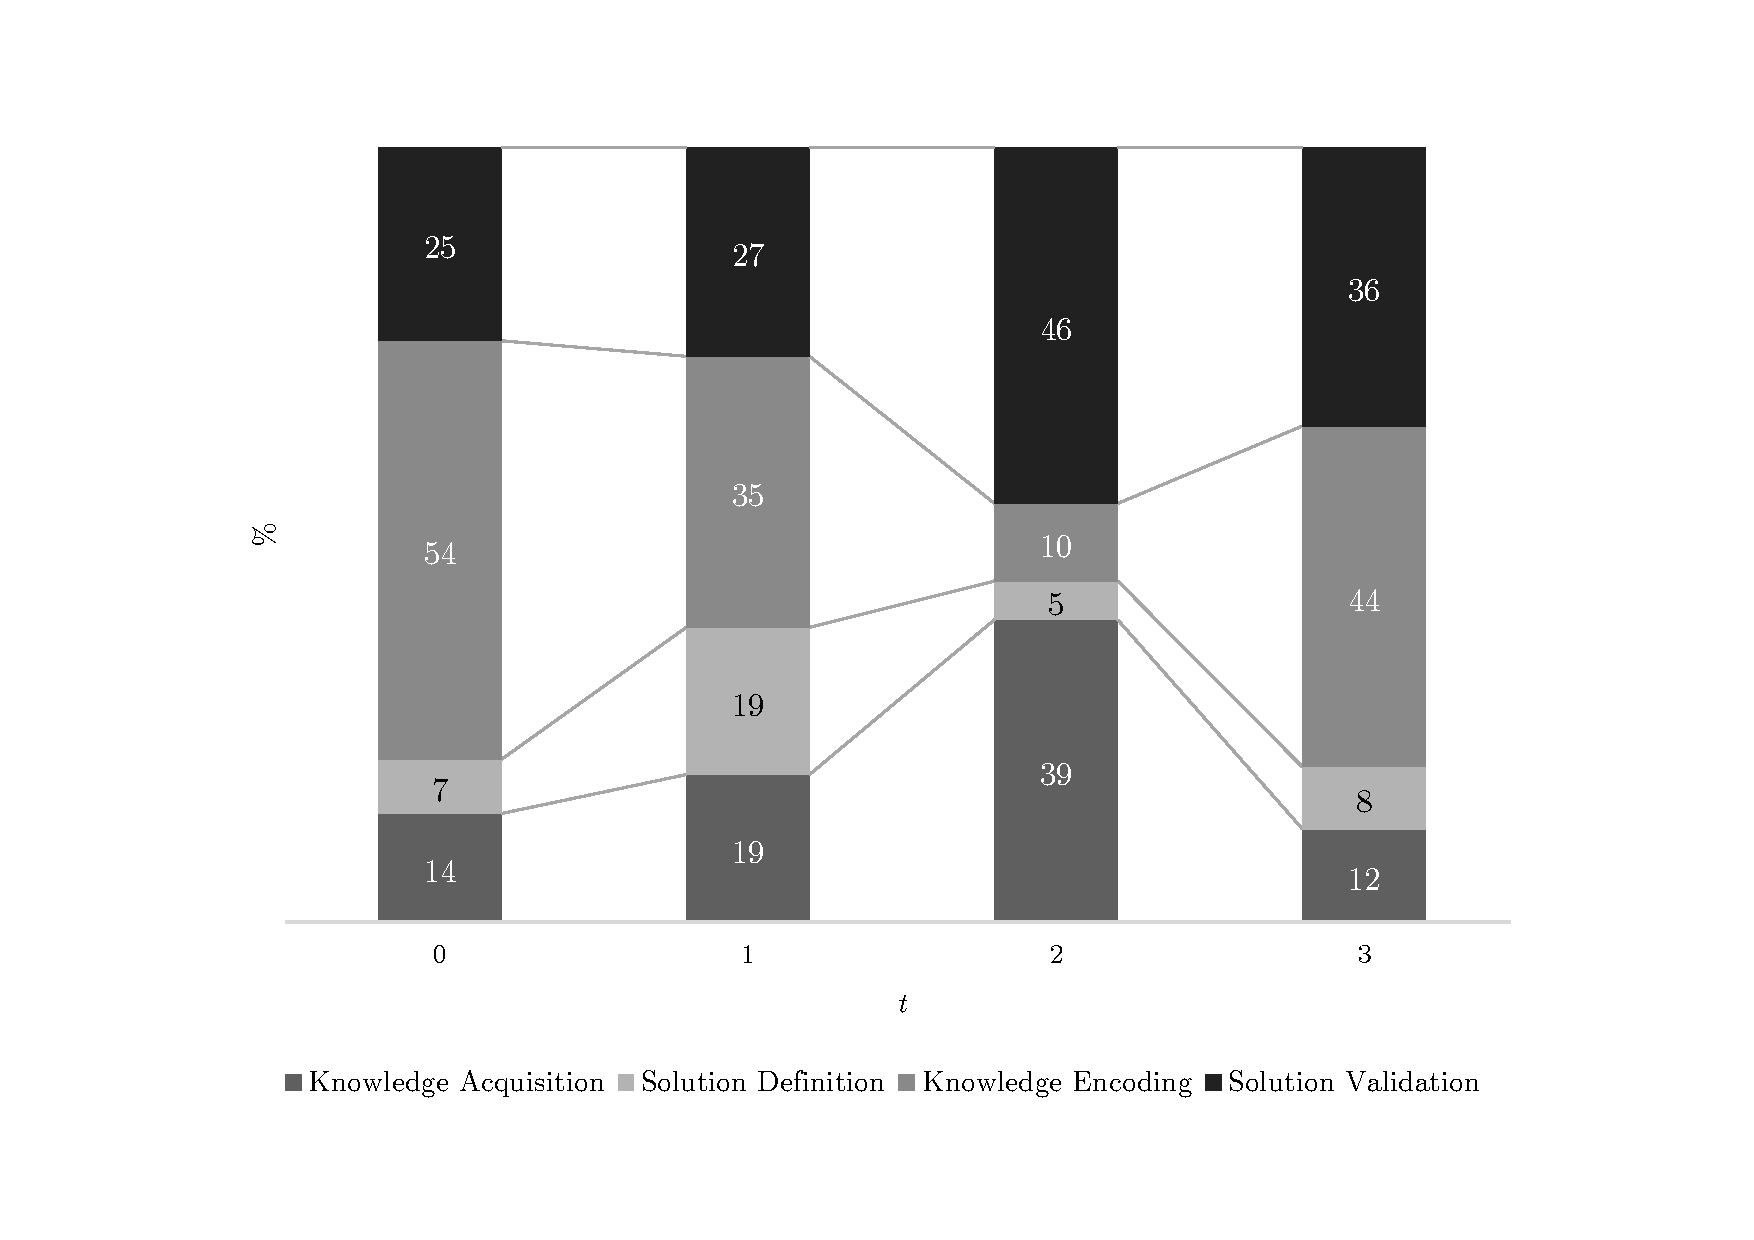
\includegraphics[height=0.65\textwidth]{graphs/percentage2.pdf}
\caption{Changes in effort as proportion of whole (including outlier)}
\label{fig:effort1}
\end{figure}

\begin{figure}
\centering
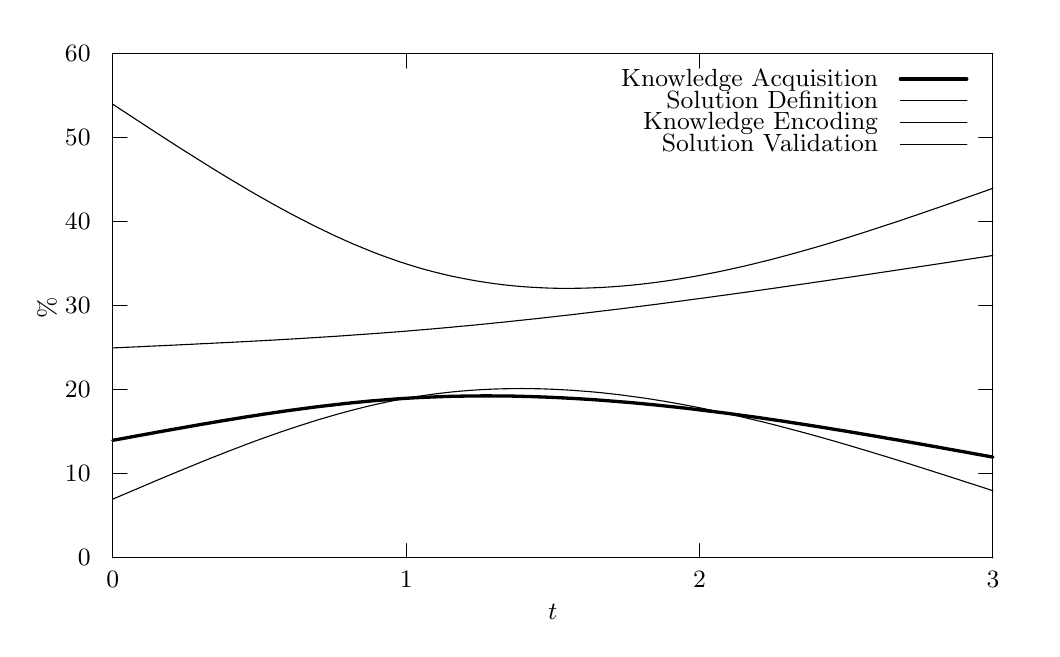
\begin{tikzpicture}[gnuplot]
%% generated with GNUPLOT 4.6p4 (Lua 5.1; terminal rev. 99, script rev. 100)
%% Fri 03 Oct 2014 12:39:55 WST
\tikzset{every node/.append style={font={\fontsize{9pt}{10.8pt}\selectfont}}}
\gpmonochromelines
\path (0.000,0.000) rectangle (12.700,7.620);
\gpcolor{color=gp lt color border}
\gpsetlinetype{gp lt border}
\gpsetlinewidth{1.00}
\draw[gp path] (1.024,0.886)--(1.204,0.886);
\draw[gp path] (12.201,0.886)--(12.021,0.886);
\node[gp node right] at (0.858,0.886) {0};
\draw[gp path] (1.024,1.953)--(1.204,1.953);
\draw[gp path] (12.201,1.953)--(12.021,1.953);
\node[gp node right] at (0.858,1.953) {10};
\draw[gp path] (1.024,3.020)--(1.204,3.020);
\draw[gp path] (12.201,3.020)--(12.021,3.020);
\node[gp node right] at (0.858,3.020) {20};
\draw[gp path] (1.024,4.087)--(1.204,4.087);
\draw[gp path] (12.201,4.087)--(12.021,4.087);
\node[gp node right] at (0.858,4.087) {30};
\draw[gp path] (1.024,5.153)--(1.204,5.153);
\draw[gp path] (12.201,5.153)--(12.021,5.153);
\node[gp node right] at (0.858,5.153) {40};
\draw[gp path] (1.024,6.220)--(1.204,6.220);
\draw[gp path] (12.201,6.220)--(12.021,6.220);
\node[gp node right] at (0.858,6.220) {50};
\draw[gp path] (1.024,7.287)--(1.204,7.287);
\draw[gp path] (12.201,7.287)--(12.021,7.287);
\node[gp node right] at (0.858,7.287) {60};
\draw[gp path] (1.024,0.886)--(1.024,1.066);
\draw[gp path] (1.024,7.287)--(1.024,7.107);
\node[gp node center] at (1.024,0.609) {0};
\draw[gp path] (4.750,0.886)--(4.750,1.066);
\draw[gp path] (4.750,7.287)--(4.750,7.107);
\node[gp node center] at (4.750,0.609) {1};
\draw[gp path] (8.475,0.886)--(8.475,1.066);
\draw[gp path] (8.475,7.287)--(8.475,7.107);
\node[gp node center] at (8.475,0.609) {2};
\draw[gp path] (12.201,0.886)--(12.201,1.066);
\draw[gp path] (12.201,7.287)--(12.201,7.107);
\node[gp node center] at (12.201,0.609) {3};
\draw[gp path] (1.024,7.287)--(1.024,0.886)--(12.201,0.886)--(12.201,7.287)--cycle;
\node[gp node center,rotate=-270] at (0.221,4.086) {\%};
\node[gp node center] at (6.612,0.194) {$t$};
\node[gp node right] at (10.859,6.969) {Knowledge Acquisition};
\gpcolor{color=gp lt color 0}
\gpsetlinetype{gp lt plot 0}
\gpsetlinewidth{3.00}
\draw[gp path] (11.025,6.969)--(11.869,6.969);
\draw[gp path] (1.024,2.380)--(1.137,2.400)--(1.250,2.421)--(1.363,2.442)--(1.476,2.462)%
  --(1.588,2.483)--(1.701,2.503)--(1.814,2.523)--(1.927,2.543)--(2.040,2.563)--(2.153,2.583)%
  --(2.266,2.602)--(2.379,2.621)--(2.492,2.640)--(2.605,2.658)--(2.717,2.677)--(2.830,2.694)%
  --(2.943,2.712)--(3.056,2.728)--(3.169,2.745)--(3.282,2.761)--(3.395,2.776)--(3.508,2.791)%
  --(3.621,2.806)--(3.734,2.819)--(3.846,2.832)--(3.959,2.845)--(4.072,2.857)--(4.185,2.868)%
  --(4.298,2.879)--(4.411,2.888)--(4.524,2.897)--(4.637,2.906)--(4.750,2.913)--(4.863,2.920)%
  --(4.975,2.925)--(5.088,2.930)--(5.201,2.934)--(5.314,2.938)--(5.427,2.940)--(5.540,2.942)%
  --(5.653,2.943)--(5.766,2.944)--(5.879,2.943)--(5.992,2.942)--(6.104,2.941)--(6.217,2.938)%
  --(6.330,2.935)--(6.443,2.931)--(6.556,2.927)--(6.669,2.922)--(6.782,2.916)--(6.895,2.910)%
  --(7.008,2.903)--(7.121,2.896)--(7.233,2.888)--(7.346,2.879)--(7.459,2.870)--(7.572,2.861)%
  --(7.685,2.851)--(7.798,2.840)--(7.911,2.829)--(8.024,2.817)--(8.137,2.805)--(8.250,2.793)%
  --(8.362,2.780)--(8.475,2.766)--(8.588,2.752)--(8.701,2.738)--(8.814,2.724)--(8.927,2.709)%
  --(9.040,2.693)--(9.153,2.678)--(9.266,2.662)--(9.379,2.645)--(9.491,2.629)--(9.604,2.612)%
  --(9.717,2.594)--(9.830,2.577)--(9.943,2.559)--(10.056,2.541)--(10.169,2.522)--(10.282,2.504)%
  --(10.395,2.485)--(10.508,2.466)--(10.620,2.447)--(10.733,2.428)--(10.846,2.408)--(10.959,2.389)%
  --(11.072,2.369)--(11.185,2.349)--(11.298,2.329)--(11.411,2.309)--(11.524,2.289)--(11.637,2.268)%
  --(11.749,2.248)--(11.862,2.228)--(11.975,2.207)--(12.088,2.187)--(12.201,2.166);
\gpcolor{color=gp lt color border}
\node[gp node right] at (10.859,6.692) {Solution Definition};
\gpcolor{color=gp lt color 1}
\gpsetlinetype{gp lt plot 1}
\gpsetlinewidth{1.00}
\draw[gp path] (11.025,6.692)--(11.869,6.692);
\draw[gp path] (1.024,1.633)--(1.137,1.681)--(1.250,1.729)--(1.363,1.777)--(1.476,1.825)%
  --(1.588,1.873)--(1.701,1.920)--(1.814,1.967)--(1.927,2.014)--(2.040,2.060)--(2.153,2.106)%
  --(2.266,2.152)--(2.379,2.196)--(2.492,2.241)--(2.605,2.284)--(2.717,2.327)--(2.830,2.369)%
  --(2.943,2.410)--(3.056,2.450)--(3.169,2.490)--(3.282,2.528)--(3.395,2.565)--(3.508,2.601)%
  --(3.621,2.637)--(3.734,2.670)--(3.846,2.703)--(3.959,2.734)--(4.072,2.764)--(4.185,2.793)%
  --(4.298,2.820)--(4.411,2.846)--(4.524,2.870)--(4.637,2.892)--(4.750,2.913)--(4.863,2.932)%
  --(4.975,2.949)--(5.088,2.965)--(5.201,2.979)--(5.314,2.992)--(5.427,3.003)--(5.540,3.012)%
  --(5.653,3.020)--(5.766,3.026)--(5.879,3.031)--(5.992,3.034)--(6.104,3.036)--(6.217,3.037)%
  --(6.330,3.036)--(6.443,3.034)--(6.556,3.030)--(6.669,3.025)--(6.782,3.019)--(6.895,3.012)%
  --(7.008,3.003)--(7.121,2.994)--(7.233,2.983)--(7.346,2.971)--(7.459,2.958)--(7.572,2.943)%
  --(7.685,2.928)--(7.798,2.912)--(7.911,2.894)--(8.024,2.876)--(8.137,2.856)--(8.250,2.836)%
  --(8.362,2.815)--(8.475,2.793)--(8.588,2.770)--(8.701,2.746)--(8.814,2.722)--(8.927,2.696)%
  --(9.040,2.670)--(9.153,2.643)--(9.266,2.616)--(9.379,2.588)--(9.491,2.559)--(9.604,2.529)%
  --(9.717,2.499)--(9.830,2.469)--(9.943,2.438)--(10.056,2.406)--(10.169,2.374)--(10.282,2.341)%
  --(10.395,2.308)--(10.508,2.274)--(10.620,2.241)--(10.733,2.206)--(10.846,2.172)--(10.959,2.137)%
  --(11.072,2.102)--(11.185,2.066)--(11.298,2.030)--(11.411,1.994)--(11.524,1.958)--(11.637,1.922)%
  --(11.749,1.886)--(11.862,1.849)--(11.975,1.813)--(12.088,1.776)--(12.201,1.739);
\gpcolor{color=gp lt color border}
\node[gp node right] at (10.859,6.415) {Knowledge Encoding};
\gpcolor{color=gp lt color 2}
\gpsetlinetype{gp lt plot 2}
\draw[gp path] (11.025,6.415)--(11.869,6.415);
\draw[gp path] (1.024,6.647)--(1.137,6.573)--(1.250,6.499)--(1.363,6.425)--(1.476,6.351)%
  --(1.588,6.278)--(1.701,6.205)--(1.814,6.132)--(1.927,6.060)--(2.040,5.989)--(2.153,5.918)%
  --(2.266,5.847)--(2.379,5.778)--(2.492,5.709)--(2.605,5.642)--(2.717,5.575)--(2.830,5.509)%
  --(2.943,5.445)--(3.056,5.381)--(3.169,5.319)--(3.282,5.258)--(3.395,5.199)--(3.508,5.141)%
  --(3.621,5.084)--(3.734,5.030)--(3.846,4.976)--(3.959,4.925)--(4.072,4.875)--(4.185,4.828)%
  --(4.298,4.782)--(4.411,4.738)--(4.524,4.697)--(4.637,4.657)--(4.750,4.620)--(4.863,4.585)%
  --(4.975,4.552)--(5.088,4.522)--(5.201,4.494)--(5.314,4.467)--(5.427,4.444)--(5.540,4.422)%
  --(5.653,4.402)--(5.766,4.384)--(5.879,4.368)--(5.992,4.354)--(6.104,4.342)--(6.217,4.332)%
  --(6.330,4.324)--(6.443,4.318)--(6.556,4.313)--(6.669,4.310)--(6.782,4.309)--(6.895,4.310)%
  --(7.008,4.312)--(7.121,4.316)--(7.233,4.321)--(7.346,4.328)--(7.459,4.336)--(7.572,4.346)%
  --(7.685,4.357)--(7.798,4.370)--(7.911,4.384)--(8.024,4.399)--(8.137,4.416)--(8.250,4.434)%
  --(8.362,4.453)--(8.475,4.473)--(8.588,4.495)--(8.701,4.517)--(8.814,4.541)--(8.927,4.566)%
  --(9.040,4.591)--(9.153,4.618)--(9.266,4.646)--(9.379,4.674)--(9.491,4.704)--(9.604,4.734)%
  --(9.717,4.765)--(9.830,4.797)--(9.943,4.829)--(10.056,4.862)--(10.169,4.896)--(10.282,4.931)%
  --(10.395,4.966)--(10.508,5.002)--(10.620,5.038)--(10.733,5.075)--(10.846,5.112)--(10.959,5.149)%
  --(11.072,5.187)--(11.185,5.225)--(11.298,5.264)--(11.411,5.303)--(11.524,5.342)--(11.637,5.381)%
  --(11.749,5.421)--(11.862,5.461)--(11.975,5.500)--(12.088,5.540)--(12.201,5.580);
\gpcolor{color=gp lt color border}
\node[gp node right] at (10.859,6.138) {Solution Validation};
\gpcolor{color=gp lt color 3}
\gpsetlinetype{gp lt plot 3}
\draw[gp path] (11.025,6.138)--(11.869,6.138);
\draw[gp path] (1.024,3.553)--(1.137,3.558)--(1.250,3.563)--(1.363,3.568)--(1.476,3.574)%
  --(1.588,3.579)--(1.701,3.584)--(1.814,3.589)--(1.927,3.595)--(2.040,3.600)--(2.153,3.606)%
  --(2.266,3.611)--(2.379,3.617)--(2.492,3.622)--(2.605,3.628)--(2.717,3.634)--(2.830,3.640)%
  --(2.943,3.646)--(3.056,3.652)--(3.169,3.659)--(3.282,3.665)--(3.395,3.672)--(3.508,3.679)%
  --(3.621,3.686)--(3.734,3.693)--(3.846,3.700)--(3.959,3.708)--(4.072,3.716)--(4.185,3.724)%
  --(4.298,3.732)--(4.411,3.740)--(4.524,3.749)--(4.637,3.757)--(4.750,3.766)--(4.863,3.776)%
  --(4.975,3.785)--(5.088,3.795)--(5.201,3.805)--(5.314,3.815)--(5.427,3.826)--(5.540,3.836)%
  --(5.653,3.847)--(5.766,3.858)--(5.879,3.870)--(5.992,3.881)--(6.104,3.893)--(6.217,3.905)%
  --(6.330,3.917)--(6.443,3.929)--(6.556,3.942)--(6.669,3.955)--(6.782,3.967)--(6.895,3.980)%
  --(7.008,3.994)--(7.121,4.007)--(7.233,4.021)--(7.346,4.034)--(7.459,4.048)--(7.572,4.062)%
  --(7.685,4.077)--(7.798,4.091)--(7.911,4.105)--(8.024,4.120)--(8.137,4.135)--(8.250,4.150)%
  --(8.362,4.165)--(8.475,4.180)--(8.588,4.195)--(8.701,4.211)--(8.814,4.226)--(8.927,4.242)%
  --(9.040,4.257)--(9.153,4.273)--(9.266,4.289)--(9.379,4.305)--(9.491,4.321)--(9.604,4.338)%
  --(9.717,4.354)--(9.830,4.370)--(9.943,4.387)--(10.056,4.403)--(10.169,4.420)--(10.282,4.437)%
  --(10.395,4.453)--(10.508,4.470)--(10.620,4.487)--(10.733,4.504)--(10.846,4.521)--(10.959,4.538)%
  --(11.072,4.555)--(11.185,4.572)--(11.298,4.589)--(11.411,4.606)--(11.524,4.623)--(11.637,4.640)%
  --(11.749,4.658)--(11.862,4.675)--(11.975,4.692)--(12.088,4.709)--(12.201,4.727);
\gpcolor{color=gp lt color border}
\gpsetlinetype{gp lt border}
\draw[gp path] (1.024,7.287)--(1.024,0.886)--(12.201,0.886)--(12.201,7.287)--cycle;
%% coordinates of the plot area
\gpdefrectangularnode{gp plot 1}{\pgfpoint{1.024cm}{0.886cm}}{\pgfpoint{12.201cm}{7.287cm}}
\end{tikzpicture}
%% gnuplot variables

\caption{Changes in effort excluding outlier}
\label{fig:effort2}
\end{figure}

\subsection{Work Variation \& Major Shifts}
In my personal development for the provided problems, there were several areas in which variation in effort were introduced. The primary area, which has been discussed at length thus far, was for $t=2$, in which due to a misunderstanding, the problem complexity was made artificially harder through the introduction of complex spherical geometry calculations. This significantly inflated the amount of effort as my knowledge of the problem was severely reduced.

Excluding that point, overall the effort across the problems reduced, as my knowledge of the problem, as well as the resources had increased far more than the problem size and complexity. This downward trend can be seen in \Fref{fig:myexcl-totalplot} and within the data of \Fref{tab:complexities}.

\Fref{fig:effort1} shows the changing proportion of the project spend in each of the broad categories of work. I converted the data of my personal process to the specified four broader categories for ease of presentation (how this conversion occurred can be seen in appendix \fref{sec:programs}).

Within the figure, we can see that from $t=0$ to $t=1$, the knowledge encoding phase decreased; this touches on the fact that much of the problem understanding that was gained in $t=0$ was portable to $t=1$, leading to a reduction of effort in that regard. 

The data surrounding $t=2$ clearly shows where the major issues were in that project; both the solution validation and the knowledge encoding phases of that project ballooned out of proportion. Both of these were due to misunderstandings as to the units used in many of the spherical geometry equations found to assist with the solution; much iteration was done to determine what these units were and what conversions were required to get to them.

Beyond those discussed areas, if one excludes $t=2$, there is no more than a 12\% variation between each stage, which can be attributed to fluctuations in problem difficulty and particular pitfalls.

Only one particular trend could be noticed with these data points (even excluding $t=2$); that is the solution valuation as a proportion is slowly increasing (see \fref{fig:effort2}). It is hard to say if this is an actual trend, or just a data anomaly. One hypothesis is that the tutorial sessions that the program is coded in have something to do with it; if there is a set amount of time in which people wish to finish the program, if people finish early, they might spend some of the remaining time ensuring that the program operates correctly. If more trend information was wishing to be derived, then a much larger data set would need to be used.

\subsection{Personal Process Evolution}
\label{subsec:personalprocesseval}
  \begin{figure}
    \centering
   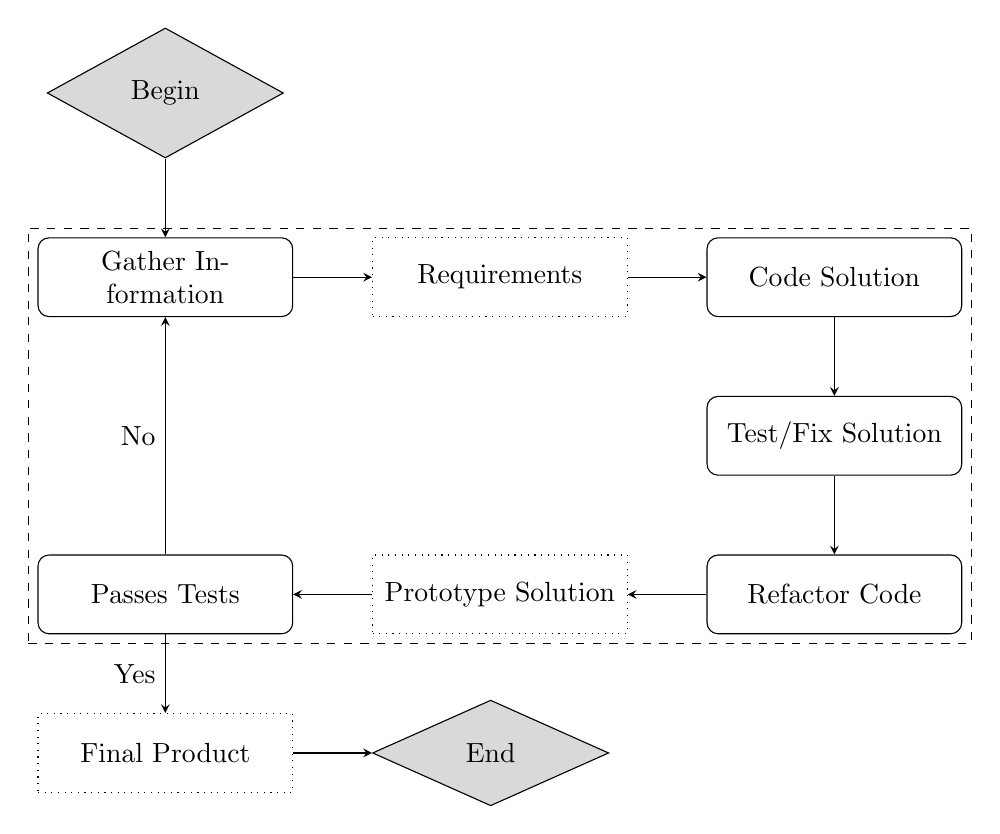
\begin{tikzpicture}[node distance=1cm]

    \node (start) [startstop] {Begin};

    \node (gather) [stepa, below=of start] {Gather Information};
    % \node (client) [infosource, below=of gather] {Client};
    \node (probdef) [outcome, right=of gather] {Requirements};


    \node (code) [stepa, right=of probdef] {Code Solution};
    \node (test) [stepa, below=of code] {Test/Fix Solution};
    \node (refactor) [stepa, below=of test] {Refactor Code};
    \node (prototype) [outcome, left=of refactor] {Prototype Solution};
    \node (feedback) [stepa, left=of prototype] {Passes Tests};


    \node[phase, fit=(gather) (code) (test) (refactor) (prototype) (feedback)] {};

    \node (final) [outcome, below=of feedback] {Final Product};
    \node (stop) [startstop, right=of final] {End};


    % \draw [arrow] (client) -- (gather);
    % \draw [arrow] (client) -- (eval);
    % \draw [arrow] (client) -- (feedback);

    % \draw [arrow] (internet) -- (tech);

    \draw [arrow] (start) -- (gather);
    \draw [arrow] (gather) -- (probdef);
    \draw [arrow] (probdef) -- (code);
    \draw [arrow] (code) -- (test);
    \draw [arrow] (test) -- (refactor);
    \draw [arrow] (refactor) -- (prototype);
    \draw [arrow] (prototype) -- (feedback);
    \draw [arrow] (feedback) -- node[anchor=east] {Yes} (final);
    \draw [arrow] (feedback) -- node[anchor=east] {No} (gather);
    \draw [arrow] (final) -- (stop);

    \end{tikzpicture}
    \caption{Revised Personal Process}
    \label{fig:revpersonalprocess}
  \end{figure}
  
My personal process (original version shown in appendix \fref{sec:personalprocess}) has evolved significantly over the duration of the course. It was quickly realised with the application of the process to real world situations that many of the parts of the process are not observed or happen implicitly as part of other phases instead. Some of the differences observed between the ``ideal'' and real version include;
\begin{itemize}
 \item Design Options are rarely evaluated explicitly: A design option is picked, and the code is refactored throughout with changing knowledge.
 \item Technical Options are not evaluated at all with such a small problem: A language that I am proficient in was picked at the very start, and due to a ban on using third-party libraries, no further decisions of that nature needed making.
 \item The Test Solution and Fix Found Bugs parts of the process are effectively merged in practice: They form a very tight iteration in which the code is modified, a new prototype is generated, which is then tested again.
 \item Code refactoring takes place at every stage of the process: Usually when it is noticed that a particular section is a source of error or is particularly complex.
 \item Feedback is not particularly sought within these problems: As the problems have very objective answers, testing acts as the core feedback mechanism to determine if the solution is satisfactory.
\end{itemize}

A revised version of this personal process can be seen in \Fref{fig:revpersonalprocess}.


\section{Conclusion}
Four different effort models were examined to determine how easily they could model real-world data, and if any conclusions could be derived from the parameters that were produced from the fitting of those models.

The difficulties in collecting the CITS5502 real world data were discussed, and a different approach was proposed to eliminate them. Problems with an outlier in my personal CITS5502 data were discussed, an alternate data was generated to help overcome this problems to some extent.

Both the CITS8220 data provided and the CITS5502 data created were fitted against all four models, with similarly broad success in the case of Models A though C, but with utter failure in the case of Model D due to poor model design, which is discussed in some detail.

The parameters $a$, $b$ and $c$ generated from the CITS8220 fitted data were discussed in great detail, outlining the function of each of these parameters in the model, and analysing how they changed between each of the three CITS8220 problem sets provided interesting insight into how prior experience in knowledge acquisition and knowledge encoding can provide significant advantage into subsequent problems in the same problem domain or resource domain respectively.

Estimation data from the whole CITS5502 cohort was examined to attempt to draw conclusions regarding how estimation can improve over subsequent program generations, however due to Problem 2 being of significantly greater initial complexity, it is hard to draw any firm conclusions with that data. Several hypotheses were proposed as to how the data could continue to trend.

The consistency between each personal solution was also analysed within the context of Logical Lines of Code and the actual time taken, coming to the conclusion that the solutions did differ in complexity, but only significantly in the case of $t=2$.

The variation between the different personal process phases was discussed in detail, with overall (outlier excluded), little by way of obvious trend to interpret. More data was needed for a thorough analysis.

Finally, how my personal process evolved over this unit's duration was discussed, as it had significantly, and a revised model of the process was provided.


% TODO: Call  problem x t=x
% TODO: mention other models in LLOC section




%\nocite{*}
%\bibliography{references}

\clearpage
\fontsize{10pt}{12pt}\selectfont
\begin{appendices}
  \section{Personal Process}
  \label{sec:personalprocess}
  Refer to Assignment 1 for flowchart key.
  \begin{figure}[!htb]
    \centering
   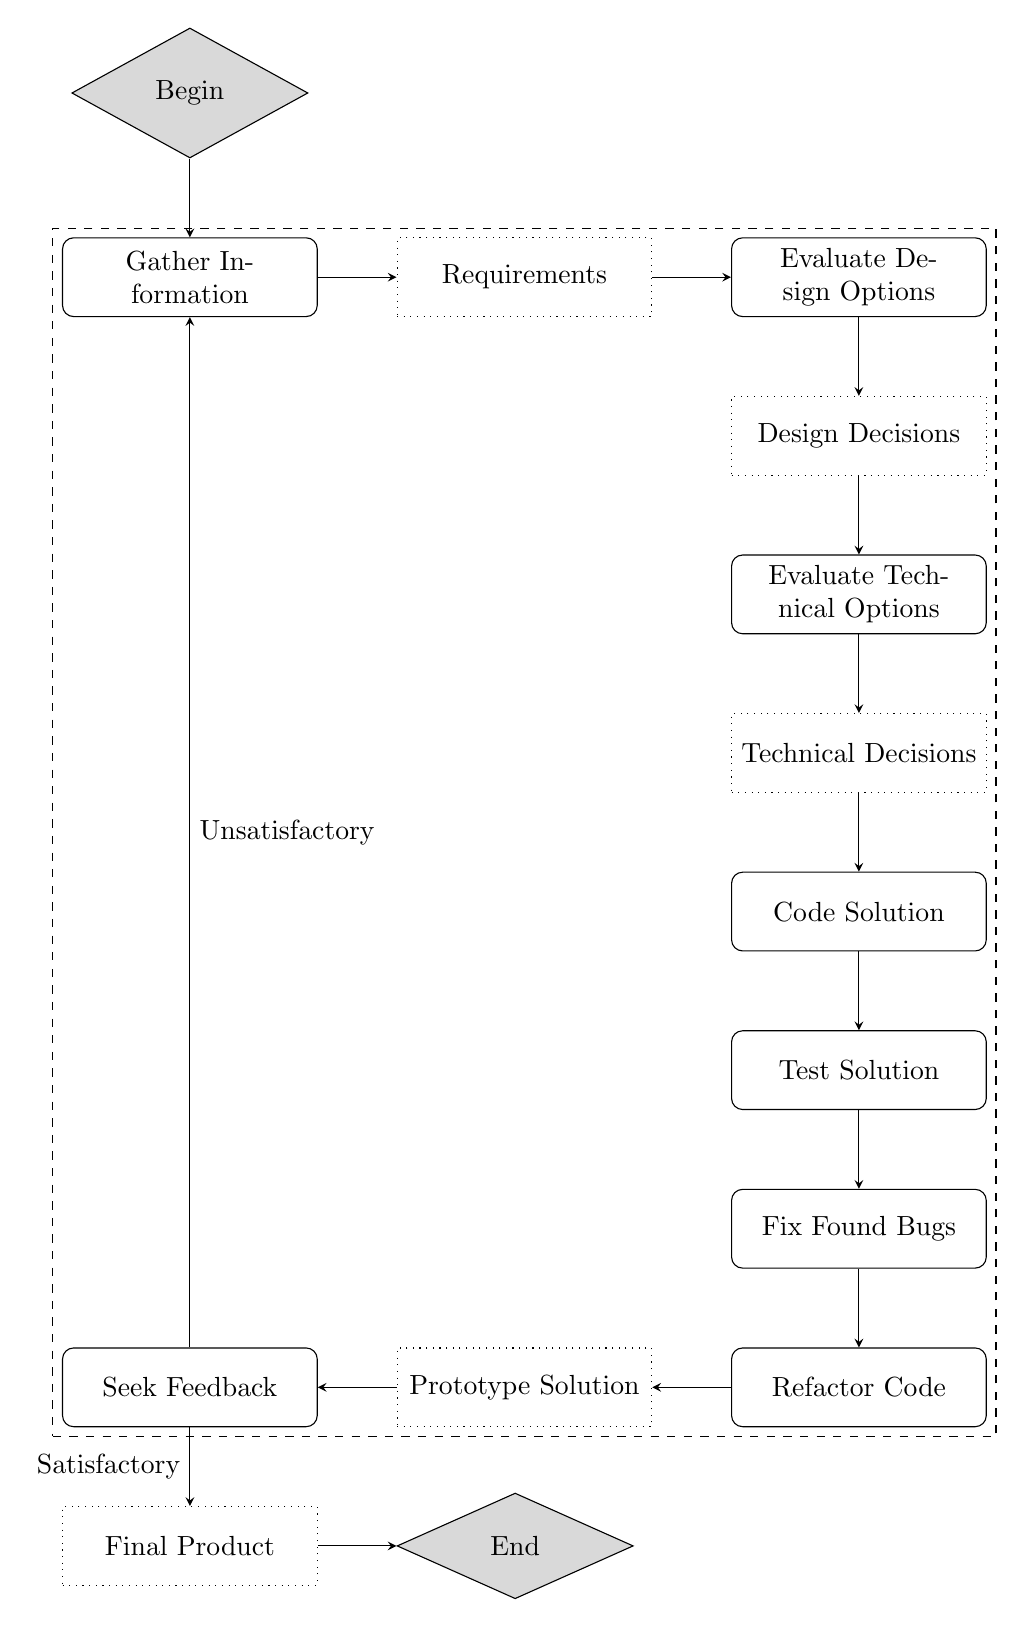
\begin{tikzpicture}[node distance=1cm]

    \node (start) [startstop] {Begin};

    \node (gather) [stepa, below=of start] {Gather Information};
    % \node (client) [infosource, below=of gather] {Client};
    \node (probdef) [outcome, right=of gather] {Requirements};
    \node (eval) [stepa, right=of probdef] {Evaluate Design Options};

    \node (designuse) [outcome, below=of eval] {Design Decisions};
    \node (tech) [stepa, below=of designuse] {Evaluate Technical Options};
    % \node (internet) [infosource, left=of tech] {Internet};
    \node (techuse) [outcome, below=of tech] {Technical Decisions};


    \node (code) [stepa, below=of techuse] {Code Solution};
    \node (test) [stepa, below=of code] {Test Solution};
    \node (bugfix) [stepa, below=of test] {Fix Found Bugs};
    \node (refactor) [stepa, below=of bugfix] {Refactor Code};
    \node (prototype) [outcome, left=of refactor] {Prototype Solution};
    \node (feedback) [stepa, left=of prototype] {Seek Feedback};


    \node[phase, fit=(gather) (code) (test) (bugfix) (refactor) (prototype) (feedback)] {};

    \node (final) [outcome, below=of feedback] {Final Product};
    \node (stop) [startstop, right=of final] {End};


    % \draw [arrow] (client) -- (gather);
    % \draw [arrow] (client) -- (eval);
    % \draw [arrow] (client) -- (feedback);

    % \draw [arrow] (internet) -- (tech);

    \draw [arrow] (start) -- (gather);
    \draw [arrow] (gather) -- (probdef);
    \draw [arrow] (probdef) -- (eval);
    \draw [arrow] (eval) -- (designuse);
    \draw [arrow] (designuse) -- (tech);
    \draw [arrow] (tech) -- (techuse);
    \draw [arrow] (techuse) -- (code);
    \draw [arrow] (code) -- (test);
    \draw [arrow] (test) -- (bugfix);
    \draw [arrow] (bugfix) -- (refactor);
    \draw [arrow] (refactor) -- (prototype);
    \draw [arrow] (prototype) -- (feedback);
    \draw [arrow] (feedback) -- node[anchor=east] {Satisfactory} (final);
    \draw [arrow] (feedback) -- node[anchor=west] {Unsatisfactory} (gather);
    \draw [arrow] (final) -- (stop);

    \end{tikzpicture}
    \caption{Personal Process}
    \label{fig:personalprocess}
  \end{figure}

  \clearpage
  \section{Personal Results}
  \label{sec:personalresults}
  
  \begin{figure}[!htb]
  \centering
  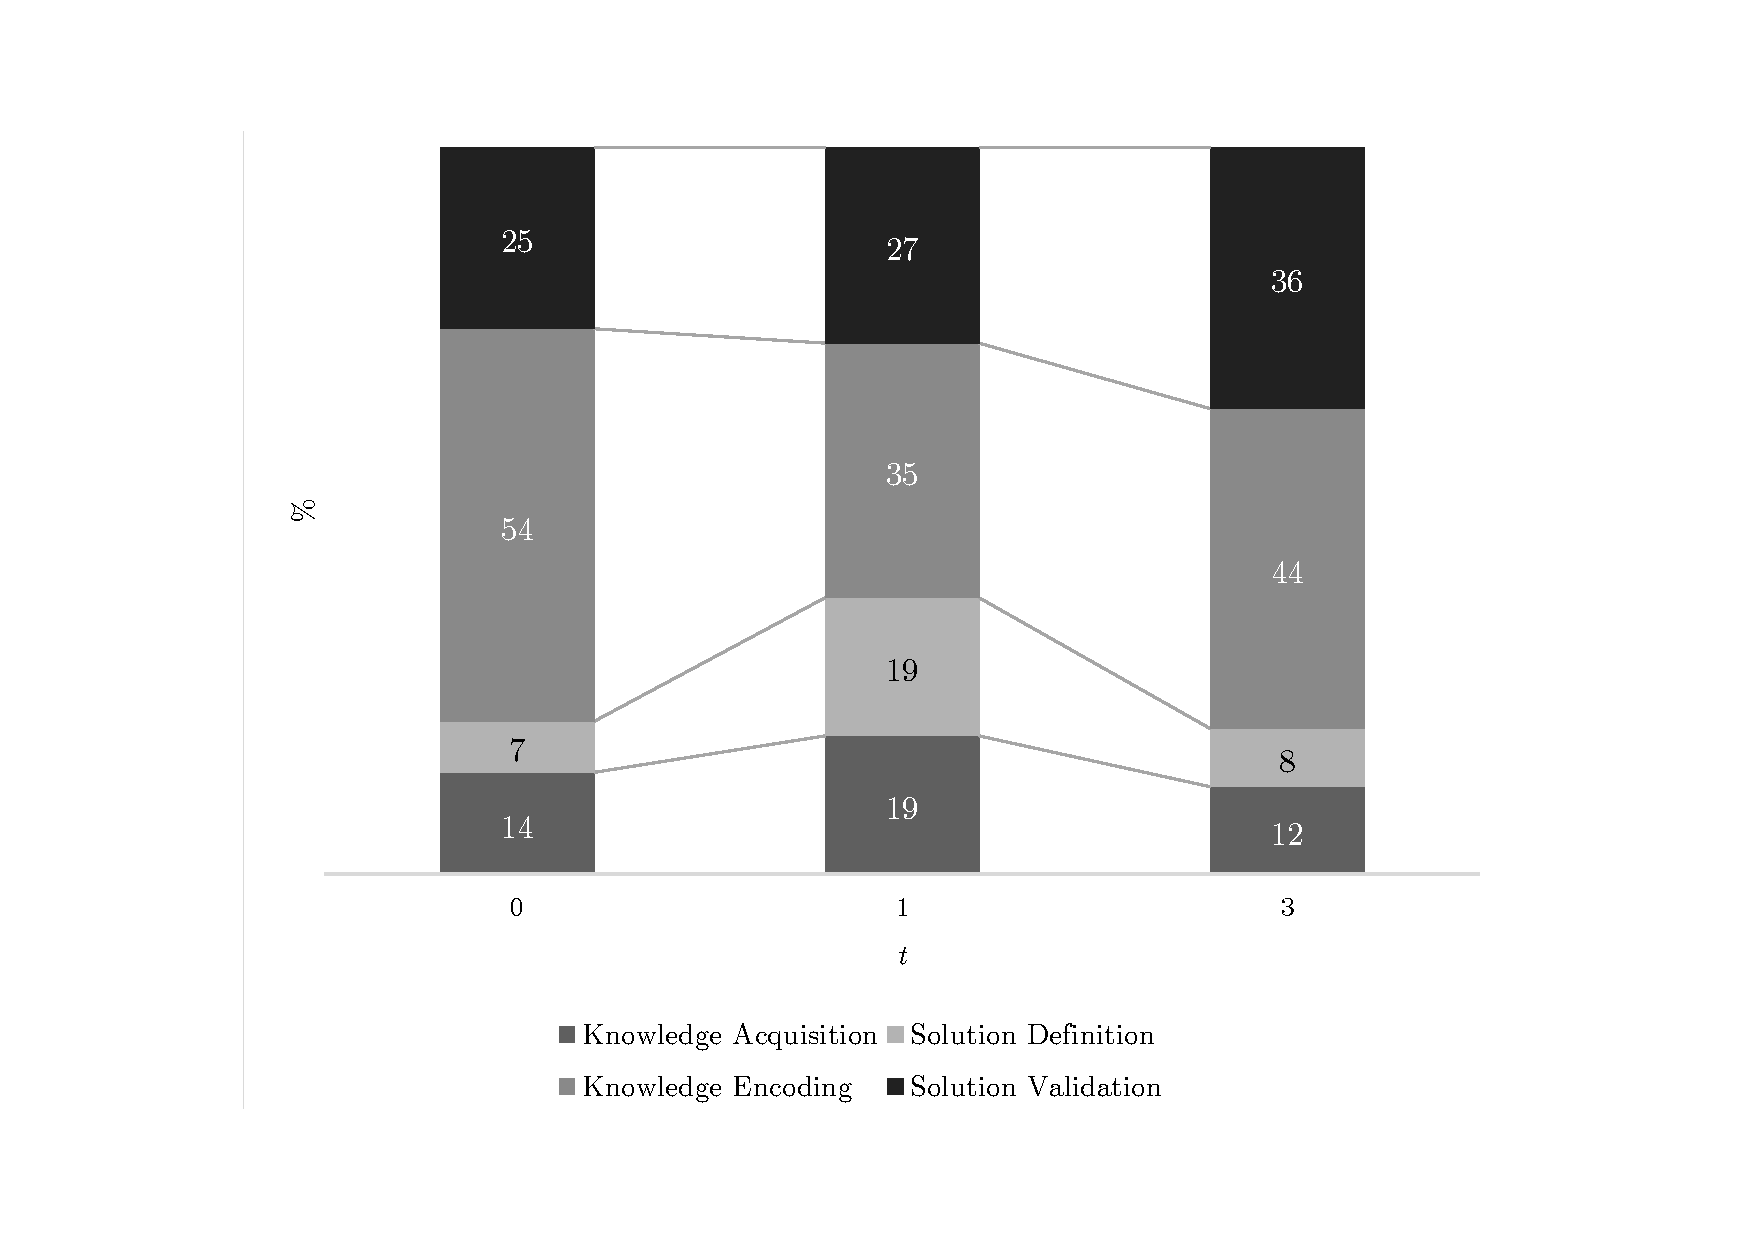
\includegraphics[height=0.65\textwidth]{graphs/percentage3.pdf}
  \caption{Changes in effort as proportion of whole (excluding outlier)}
  \end{figure}

  \begin{figure}[!htb]
  \centering
  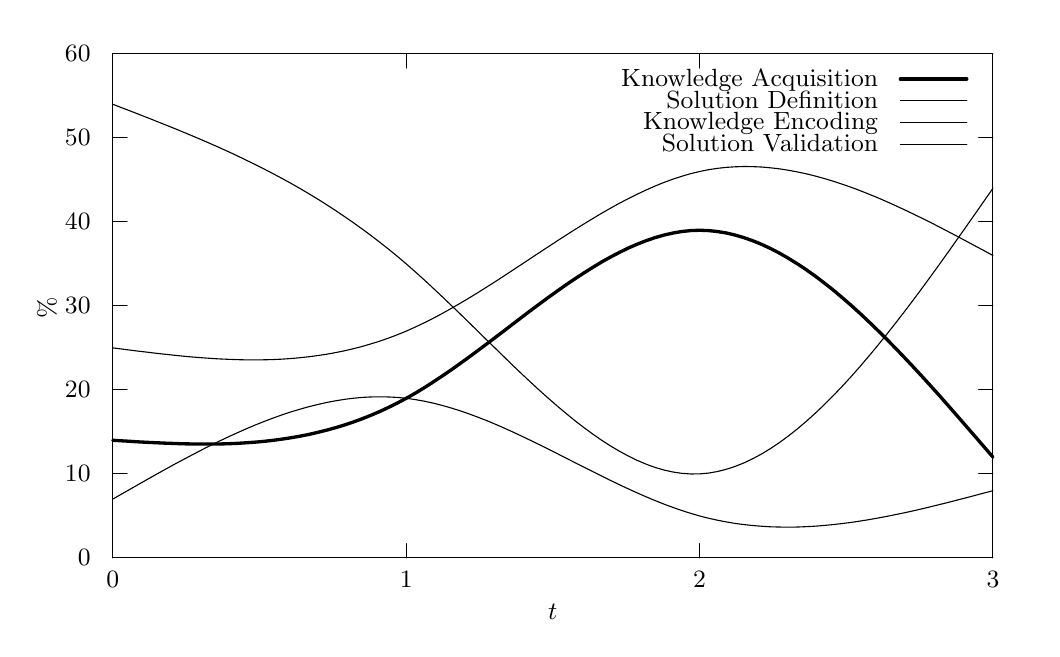
\begin{tikzpicture}[gnuplot]
%% generated with GNUPLOT 4.6p4 (Lua 5.1; terminal rev. 99, script rev. 100)
%% Fri 03 Oct 2014 12:39:55 WST
\tikzset{every node/.append style={font={\fontsize{9pt}{10.8pt}\selectfont}}}
\gpmonochromelines
\path (0.000,0.000) rectangle (12.700,7.620);
\gpcolor{color=gp lt color border}
\gpsetlinetype{gp lt border}
\gpsetlinewidth{1.00}
\draw[gp path] (1.024,0.886)--(1.204,0.886);
\draw[gp path] (12.201,0.886)--(12.021,0.886);
\node[gp node right] at (0.858,0.886) {0};
\draw[gp path] (1.024,1.953)--(1.204,1.953);
\draw[gp path] (12.201,1.953)--(12.021,1.953);
\node[gp node right] at (0.858,1.953) {10};
\draw[gp path] (1.024,3.020)--(1.204,3.020);
\draw[gp path] (12.201,3.020)--(12.021,3.020);
\node[gp node right] at (0.858,3.020) {20};
\draw[gp path] (1.024,4.087)--(1.204,4.087);
\draw[gp path] (12.201,4.087)--(12.021,4.087);
\node[gp node right] at (0.858,4.087) {30};
\draw[gp path] (1.024,5.153)--(1.204,5.153);
\draw[gp path] (12.201,5.153)--(12.021,5.153);
\node[gp node right] at (0.858,5.153) {40};
\draw[gp path] (1.024,6.220)--(1.204,6.220);
\draw[gp path] (12.201,6.220)--(12.021,6.220);
\node[gp node right] at (0.858,6.220) {50};
\draw[gp path] (1.024,7.287)--(1.204,7.287);
\draw[gp path] (12.201,7.287)--(12.021,7.287);
\node[gp node right] at (0.858,7.287) {60};
\draw[gp path] (1.024,0.886)--(1.024,1.066);
\draw[gp path] (1.024,7.287)--(1.024,7.107);
\node[gp node center] at (1.024,0.609) {0};
\draw[gp path] (4.750,0.886)--(4.750,1.066);
\draw[gp path] (4.750,7.287)--(4.750,7.107);
\node[gp node center] at (4.750,0.609) {1};
\draw[gp path] (8.475,0.886)--(8.475,1.066);
\draw[gp path] (8.475,7.287)--(8.475,7.107);
\node[gp node center] at (8.475,0.609) {2};
\draw[gp path] (12.201,0.886)--(12.201,1.066);
\draw[gp path] (12.201,7.287)--(12.201,7.107);
\node[gp node center] at (12.201,0.609) {3};
\draw[gp path] (1.024,7.287)--(1.024,0.886)--(12.201,0.886)--(12.201,7.287)--cycle;
\node[gp node center,rotate=-270] at (0.221,4.086) {\%};
\node[gp node center] at (6.612,0.194) {$t$};
\node[gp node right] at (10.859,6.969) {Knowledge Acquisition};
\gpcolor{color=gp lt color 0}
\gpsetlinetype{gp lt plot 0}
\gpsetlinewidth{3.00}
\draw[gp path] (11.025,6.969)--(11.869,6.969);
\draw[gp path] (1.024,2.380)--(1.137,2.373)--(1.250,2.366)--(1.363,2.359)--(1.476,2.353)%
  --(1.588,2.348)--(1.701,2.343)--(1.814,2.339)--(1.927,2.335)--(2.040,2.333)--(2.153,2.332)%
  --(2.266,2.332)--(2.379,2.333)--(2.492,2.336)--(2.605,2.341)--(2.717,2.348)--(2.830,2.356)%
  --(2.943,2.366)--(3.056,2.379)--(3.169,2.394)--(3.282,2.411)--(3.395,2.431)--(3.508,2.453)%
  --(3.621,2.479)--(3.734,2.507)--(3.846,2.538)--(3.959,2.572)--(4.072,2.610)--(4.185,2.651)%
  --(4.298,2.696)--(4.411,2.744)--(4.524,2.797)--(4.637,2.853)--(4.750,2.913)--(4.863,2.977)%
  --(4.975,3.045)--(5.088,3.117)--(5.201,3.192)--(5.314,3.269)--(5.427,3.349)--(5.540,3.431)%
  --(5.653,3.514)--(5.766,3.599)--(5.879,3.684)--(5.992,3.770)--(6.104,3.856)--(6.217,3.942)%
  --(6.330,4.028)--(6.443,4.112)--(6.556,4.195)--(6.669,4.276)--(6.782,4.356)--(6.895,4.432)%
  --(7.008,4.506)--(7.121,4.577)--(7.233,4.645)--(7.346,4.708)--(7.459,4.767)--(7.572,4.822)%
  --(7.685,4.871)--(7.798,4.915)--(7.911,4.954)--(8.024,4.986)--(8.137,5.012)--(8.250,5.031)%
  --(8.362,5.043)--(8.475,5.047)--(8.588,5.043)--(8.701,5.031)--(8.814,5.013)--(8.927,4.986)%
  --(9.040,4.953)--(9.153,4.913)--(9.266,4.867)--(9.379,4.814)--(9.491,4.756)--(9.604,4.691)%
  --(9.717,4.621)--(9.830,4.546)--(9.943,4.466)--(10.056,4.380)--(10.169,4.291)--(10.282,4.196)%
  --(10.395,4.098)--(10.508,3.996)--(10.620,3.890)--(10.733,3.781)--(10.846,3.669)--(10.959,3.554)%
  --(11.072,3.436)--(11.185,3.316)--(11.298,3.194)--(11.411,3.070)--(11.524,2.944)--(11.637,2.816)%
  --(11.749,2.688)--(11.862,2.558)--(11.975,2.428)--(12.088,2.297)--(12.201,2.166);
\gpcolor{color=gp lt color border}
\node[gp node right] at (10.859,6.692) {Solution Definition};
\gpcolor{color=gp lt color 1}
\gpsetlinetype{gp lt plot 1}
\gpsetlinewidth{1.00}
\draw[gp path] (11.025,6.692)--(11.869,6.692);
\draw[gp path] (1.024,1.633)--(1.137,1.698)--(1.250,1.762)--(1.363,1.827)--(1.476,1.891)%
  --(1.588,1.954)--(1.701,2.017)--(1.814,2.079)--(1.927,2.139)--(2.040,2.199)--(2.153,2.258)%
  --(2.266,2.315)--(2.379,2.370)--(2.492,2.424)--(2.605,2.475)--(2.717,2.525)--(2.830,2.573)%
  --(2.943,2.618)--(3.056,2.661)--(3.169,2.701)--(3.282,2.739)--(3.395,2.773)--(3.508,2.805)%
  --(3.621,2.833)--(3.734,2.859)--(3.846,2.880)--(3.959,2.899)--(4.072,2.913)--(4.185,2.924)%
  --(4.298,2.930)--(4.411,2.932)--(4.524,2.930)--(4.637,2.924)--(4.750,2.913)--(4.863,2.897)%
  --(4.975,2.877)--(5.088,2.853)--(5.201,2.824)--(5.314,2.792)--(5.427,2.757)--(5.540,2.718)%
  --(5.653,2.676)--(5.766,2.632)--(5.879,2.585)--(5.992,2.536)--(6.104,2.485)--(6.217,2.432)%
  --(6.330,2.378)--(6.443,2.323)--(6.556,2.267)--(6.669,2.210)--(6.782,2.152)--(6.895,2.095)%
  --(7.008,2.038)--(7.121,1.981)--(7.233,1.925)--(7.346,1.869)--(7.459,1.815)--(7.572,1.762)%
  --(7.685,1.711)--(7.798,1.661)--(7.911,1.614)--(8.024,1.569)--(8.137,1.527)--(8.250,1.488)%
  --(8.362,1.452)--(8.475,1.419)--(8.588,1.390)--(8.701,1.365)--(8.814,1.343)--(8.927,1.324)%
  --(9.040,1.309)--(9.153,1.297)--(9.266,1.288)--(9.379,1.281)--(9.491,1.278)--(9.604,1.277)%
  --(9.717,1.278)--(9.830,1.283)--(9.943,1.289)--(10.056,1.298)--(10.169,1.309)--(10.282,1.322)%
  --(10.395,1.336)--(10.508,1.353)--(10.620,1.371)--(10.733,1.391)--(10.846,1.412)--(10.959,1.435)%
  --(11.072,1.458)--(11.185,1.483)--(11.298,1.509)--(11.411,1.536)--(11.524,1.564)--(11.637,1.592)%
  --(11.749,1.621)--(11.862,1.650)--(11.975,1.680)--(12.088,1.710)--(12.201,1.739);
\gpcolor{color=gp lt color border}
\node[gp node right] at (10.859,6.415) {Knowledge Encoding};
\gpcolor{color=gp lt color 2}
\gpsetlinetype{gp lt plot 2}
\draw[gp path] (11.025,6.415)--(11.869,6.415);
\draw[gp path] (1.024,6.647)--(1.137,6.603)--(1.250,6.560)--(1.363,6.516)--(1.476,6.472)%
  --(1.588,6.427)--(1.701,6.382)--(1.814,6.337)--(1.927,6.290)--(2.040,6.243)--(2.153,6.195)%
  --(2.266,6.146)--(2.379,6.096)--(2.492,6.045)--(2.605,5.992)--(2.717,5.938)--(2.830,5.883)%
  --(2.943,5.826)--(3.056,5.767)--(3.169,5.707)--(3.282,5.645)--(3.395,5.581)--(3.508,5.514)%
  --(3.621,5.446)--(3.734,5.375)--(3.846,5.302)--(3.959,5.226)--(4.072,5.148)--(4.185,5.067)%
  --(4.298,4.984)--(4.411,4.897)--(4.524,4.808)--(4.637,4.716)--(4.750,4.620)--(4.863,4.521)%
  --(4.975,4.420)--(5.088,4.315)--(5.201,4.209)--(5.314,4.101)--(5.427,3.992)--(5.540,3.882)%
  --(5.653,3.771)--(5.766,3.660)--(5.879,3.550)--(5.992,3.440)--(6.104,3.330)--(6.217,3.223)%
  --(6.330,3.117)--(6.443,3.013)--(6.556,2.912)--(6.669,2.814)--(6.782,2.719)--(6.895,2.627)%
  --(7.008,2.540)--(7.121,2.457)--(7.233,2.379)--(7.346,2.307)--(7.459,2.240)--(7.572,2.179)%
  --(7.685,2.124)--(7.798,2.076)--(7.911,2.035)--(8.024,2.002)--(8.137,1.977)--(8.250,1.960)%
  --(8.362,1.952)--(8.475,1.953)--(8.588,1.963)--(8.701,1.983)--(8.814,2.011)--(8.927,2.048)%
  --(9.040,2.093)--(9.153,2.147)--(9.266,2.208)--(9.379,2.277)--(9.491,2.352)--(9.604,2.435)%
  --(9.717,2.524)--(9.830,2.620)--(9.943,2.722)--(10.056,2.829)--(10.169,2.942)--(10.282,3.060)%
  --(10.395,3.183)--(10.508,3.311)--(10.620,3.442)--(10.733,3.578)--(10.846,3.718)--(10.959,3.861)%
  --(11.072,4.007)--(11.185,4.156)--(11.298,4.308)--(11.411,4.462)--(11.524,4.618)--(11.637,4.776)%
  --(11.749,4.935)--(11.862,5.095)--(11.975,5.256)--(12.088,5.418)--(12.201,5.580);
\gpcolor{color=gp lt color border}
\node[gp node right] at (10.859,6.138) {Solution Validation};
\gpcolor{color=gp lt color 3}
\gpsetlinetype{gp lt plot 3}
\draw[gp path] (11.025,6.138)--(11.869,6.138);
\draw[gp path] (1.024,3.553)--(1.137,3.539)--(1.250,3.524)--(1.363,3.510)--(1.476,3.497)%
  --(1.588,3.483)--(1.701,3.471)--(1.814,3.459)--(1.927,3.447)--(2.040,3.437)--(2.153,3.428)%
  --(2.266,3.420)--(2.379,3.413)--(2.492,3.408)--(2.605,3.404)--(2.717,3.401)--(2.830,3.401)%
  --(2.943,3.402)--(3.056,3.405)--(3.169,3.410)--(3.282,3.418)--(3.395,3.428)--(3.508,3.440)%
  --(3.621,3.455)--(3.734,3.472)--(3.846,3.492)--(3.959,3.515)--(4.072,3.541)--(4.185,3.570)%
  --(4.298,3.603)--(4.411,3.638)--(4.524,3.677)--(4.637,3.720)--(4.750,3.766)--(4.863,3.817)%
  --(4.975,3.870)--(5.088,3.927)--(5.201,3.987)--(5.314,4.050)--(5.427,4.115)--(5.540,4.182)%
  --(5.653,4.251)--(5.766,4.322)--(5.879,4.394)--(5.992,4.467)--(6.104,4.541)--(6.217,4.615)%
  --(6.330,4.690)--(6.443,4.765)--(6.556,4.839)--(6.669,4.913)--(6.782,4.986)--(6.895,5.058)%
  --(7.008,5.128)--(7.121,5.197)--(7.233,5.264)--(7.346,5.328)--(7.459,5.391)--(7.572,5.450)%
  --(7.685,5.506)--(7.798,5.559)--(7.911,5.609)--(8.024,5.655)--(8.137,5.696)--(8.250,5.733)%
  --(8.362,5.766)--(8.475,5.793)--(8.588,5.816)--(8.701,5.833)--(8.814,5.846)--(8.927,5.853)%
  --(9.040,5.857)--(9.153,5.855)--(9.266,5.850)--(9.379,5.840)--(9.491,5.827)--(9.604,5.809)%
  --(9.717,5.788)--(9.830,5.764)--(9.943,5.736)--(10.056,5.705)--(10.169,5.671)--(10.282,5.634)%
  --(10.395,5.595)--(10.508,5.553)--(10.620,5.508)--(10.733,5.462)--(10.846,5.413)--(10.959,5.362)%
  --(11.072,5.310)--(11.185,5.256)--(11.298,5.201)--(11.411,5.145)--(11.524,5.087)--(11.637,5.028)%
  --(11.749,4.969)--(11.862,4.909)--(11.975,4.848)--(12.088,4.788)--(12.201,4.727);
\gpcolor{color=gp lt color border}
\gpsetlinetype{gp lt border}
\draw[gp path] (1.024,7.287)--(1.024,0.886)--(12.201,0.886)--(12.201,7.287)--cycle;
%% coordinates of the plot area
\gpdefrectangularnode{gp plot 1}{\pgfpoint{1.024cm}{0.886cm}}{\pgfpoint{12.201cm}{7.287cm}}
\end{tikzpicture}
%% gnuplot variables

  \caption{Changes in effort including outlier}
  \end{figure}
 
  
  \clearpage
  \subsection{Excluding Outlier}
  \begin{figure}[!htb]
  \centering
  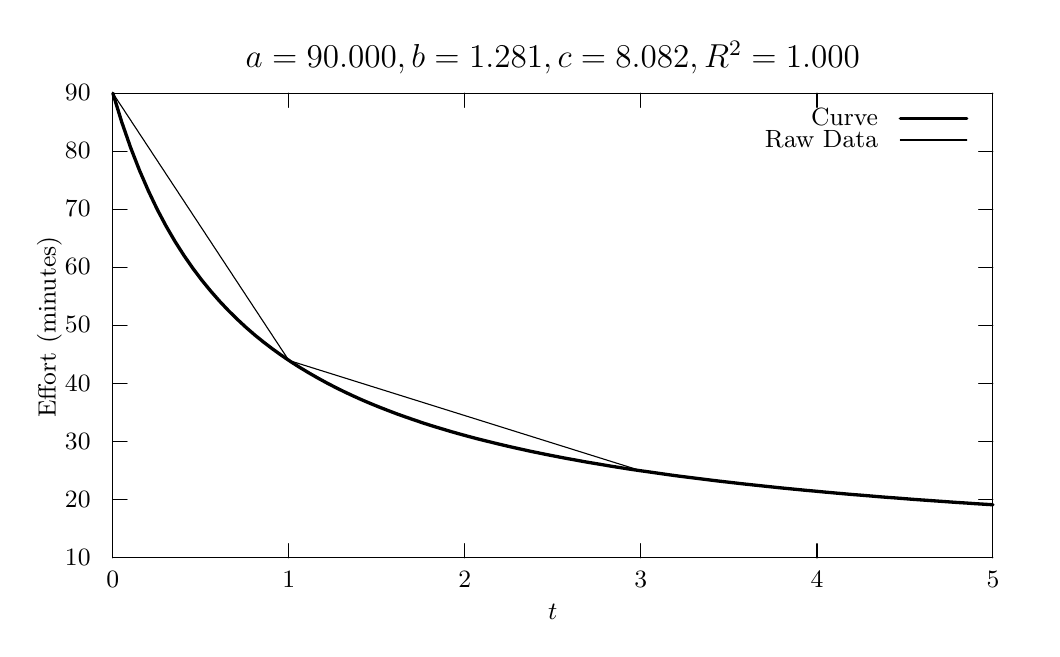
\begin{tikzpicture}[gnuplot]
%% generated with GNUPLOT 4.6p4 (Lua 5.1; terminal rev. 99, script rev. 100)
%% Fri 03 Oct 2014 12:39:55 WST
\tikzset{every node/.append style={font={\fontsize{9pt}{10.8pt}\selectfont}}}
\gpmonochromelines
\path (0.000,0.000) rectangle (12.700,7.620);
\gpcolor{color=gp lt color border}
\gpsetlinetype{gp lt border}
\gpsetlinewidth{1.00}
\draw[gp path] (1.024,0.886)--(1.204,0.886);
\draw[gp path] (12.201,0.886)--(12.021,0.886);
\node[gp node right] at (0.858,0.886) {10};
\draw[gp path] (1.024,1.624)--(1.204,1.624);
\draw[gp path] (12.201,1.624)--(12.021,1.624);
\node[gp node right] at (0.858,1.624) {20};
\draw[gp path] (1.024,2.362)--(1.204,2.362);
\draw[gp path] (12.201,2.362)--(12.021,2.362);
\node[gp node right] at (0.858,2.362) {30};
\draw[gp path] (1.024,3.099)--(1.204,3.099);
\draw[gp path] (12.201,3.099)--(12.021,3.099);
\node[gp node right] at (0.858,3.099) {40};
\draw[gp path] (1.024,3.837)--(1.204,3.837);
\draw[gp path] (12.201,3.837)--(12.021,3.837);
\node[gp node right] at (0.858,3.837) {50};
\draw[gp path] (1.024,4.575)--(1.204,4.575);
\draw[gp path] (12.201,4.575)--(12.021,4.575);
\node[gp node right] at (0.858,4.575) {60};
\draw[gp path] (1.024,5.313)--(1.204,5.313);
\draw[gp path] (12.201,5.313)--(12.021,5.313);
\node[gp node right] at (0.858,5.313) {70};
\draw[gp path] (1.024,6.050)--(1.204,6.050);
\draw[gp path] (12.201,6.050)--(12.021,6.050);
\node[gp node right] at (0.858,6.050) {80};
\draw[gp path] (1.024,6.788)--(1.204,6.788);
\draw[gp path] (12.201,6.788)--(12.021,6.788);
\node[gp node right] at (0.858,6.788) {90};
\draw[gp path] (1.024,0.886)--(1.024,1.066);
\draw[gp path] (1.024,6.788)--(1.024,6.608);
\node[gp node center] at (1.024,0.609) {0};
\draw[gp path] (3.259,0.886)--(3.259,1.066);
\draw[gp path] (3.259,6.788)--(3.259,6.608);
\node[gp node center] at (3.259,0.609) {1};
\draw[gp path] (5.495,0.886)--(5.495,1.066);
\draw[gp path] (5.495,6.788)--(5.495,6.608);
\node[gp node center] at (5.495,0.609) {2};
\draw[gp path] (7.730,0.886)--(7.730,1.066);
\draw[gp path] (7.730,6.788)--(7.730,6.608);
\node[gp node center] at (7.730,0.609) {3};
\draw[gp path] (9.966,0.886)--(9.966,1.066);
\draw[gp path] (9.966,6.788)--(9.966,6.608);
\node[gp node center] at (9.966,0.609) {4};
\draw[gp path] (12.201,0.886)--(12.201,1.066);
\draw[gp path] (12.201,6.788)--(12.201,6.608);
\node[gp node center] at (12.201,0.609) {5};
\draw[gp path] (1.024,6.788)--(1.024,0.886)--(12.201,0.886)--(12.201,6.788)--cycle;
\node[gp node center,rotate=-270] at (0.221,3.837) {Effort (minutes)};
\node[gp node center] at (6.612,0.194) {$t$};
\node[gp node center,font={\fontsize{12pt}{14.4pt}\selectfont}] at (6.612,7.204) {$a = 90.000, b = 1.281, c = 8.082, R^2 = 1.000$};
\node[gp node right] at (10.859,6.470) {Curve};
\gpcolor{color=gp lt color 0}
\gpsetlinetype{gp lt plot 0}
\gpsetlinewidth{3.00}
\draw[gp path] (11.025,6.470)--(11.869,6.470);
\draw[gp path] (1.024,6.788)--(1.137,6.421)--(1.250,6.096)--(1.363,5.806)--(1.476,5.546)%
  --(1.588,5.311)--(1.701,5.098)--(1.814,4.904)--(1.927,4.727)--(2.040,4.564)--(2.153,4.414)%
  --(2.266,4.276)--(2.379,4.147)--(2.492,4.027)--(2.605,3.916)--(2.717,3.812)--(2.830,3.714)%
  --(2.943,3.623)--(3.056,3.537)--(3.169,3.456)--(3.282,3.379)--(3.395,3.307)--(3.508,3.239)%
  --(3.621,3.174)--(3.734,3.112)--(3.846,3.054)--(3.959,2.998)--(4.072,2.945)--(4.185,2.894)%
  --(4.298,2.846)--(4.411,2.800)--(4.524,2.756)--(4.637,2.713)--(4.750,2.673)--(4.863,2.634)%
  --(4.975,2.596)--(5.088,2.560)--(5.201,2.526)--(5.314,2.492)--(5.427,2.460)--(5.540,2.429)%
  --(5.653,2.399)--(5.766,2.371)--(5.879,2.343)--(5.992,2.316)--(6.104,2.290)--(6.217,2.265)%
  --(6.330,2.240)--(6.443,2.217)--(6.556,2.194)--(6.669,2.172)--(6.782,2.150)--(6.895,2.130)%
  --(7.008,2.109)--(7.121,2.090)--(7.233,2.071)--(7.346,2.052)--(7.459,2.034)--(7.572,2.016)%
  --(7.685,1.999)--(7.798,1.983)--(7.911,1.967)--(8.024,1.951)--(8.137,1.935)--(8.250,1.920)%
  --(8.362,1.906)--(8.475,1.892)--(8.588,1.878)--(8.701,1.864)--(8.814,1.851)--(8.927,1.838)%
  --(9.040,1.825)--(9.153,1.813)--(9.266,1.801)--(9.379,1.789)--(9.491,1.777)--(9.604,1.766)%
  --(9.717,1.755)--(9.830,1.744)--(9.943,1.734)--(10.056,1.723)--(10.169,1.713)--(10.282,1.703)%
  --(10.395,1.693)--(10.508,1.684)--(10.620,1.675)--(10.733,1.665)--(10.846,1.656)--(10.959,1.648)%
  --(11.072,1.639)--(11.185,1.630)--(11.298,1.622)--(11.411,1.614)--(11.524,1.606)--(11.637,1.598)%
  --(11.749,1.590)--(11.862,1.583)--(11.975,1.575)--(12.088,1.568)--(12.201,1.561);
\gpcolor{color=gp lt color border}
\node[gp node right] at (10.859,6.193) {Raw Data};
\gpcolor{color=gp lt color 3}
\gpsetlinetype{gp lt plot 3}
\gpsetlinewidth{1.00}
\draw[gp path] (11.025,6.193)--(11.869,6.193);
\draw[gp path] (1.024,6.788)--(3.259,3.394)--(7.730,1.993);
\gpcolor{color=gp lt color border}
\gpsetlinetype{gp lt border}
\draw[gp path] (1.024,6.788)--(1.024,0.886)--(12.201,0.886)--(12.201,6.788)--cycle;
%% coordinates of the plot area
\gpdefrectangularnode{gp plot 1}{\pgfpoint{1.024cm}{0.886cm}}{\pgfpoint{12.201cm}{6.788cm}}
\end{tikzpicture}
%% gnuplot variables

  \caption{$\frac{a+bct}{bt+1}$}
  \end{figure}
  
  \begin{figure}[!htb]
  \centering
  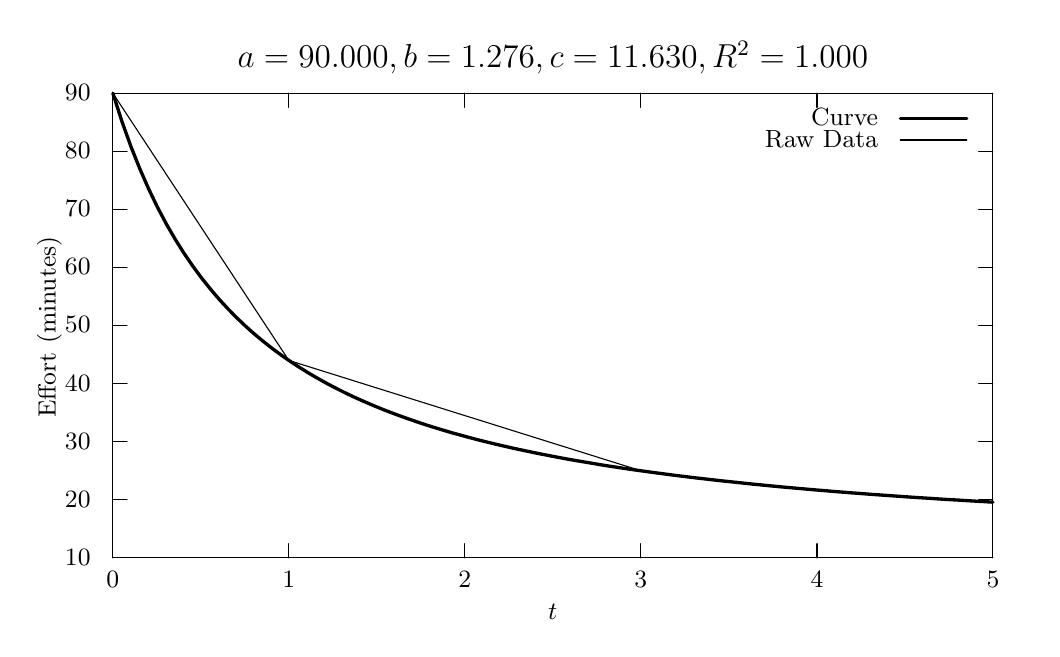
\begin{tikzpicture}[gnuplot]
%% generated with GNUPLOT 4.6p4 (Lua 5.1; terminal rev. 99, script rev. 100)
%% Fri 03 Oct 2014 12:39:55 WST
\tikzset{every node/.append style={font={\fontsize{9pt}{10.8pt}\selectfont}}}
\gpmonochromelines
\path (0.000,0.000) rectangle (12.700,7.620);
\gpcolor{color=gp lt color border}
\gpsetlinetype{gp lt border}
\gpsetlinewidth{1.00}
\draw[gp path] (1.024,0.886)--(1.204,0.886);
\draw[gp path] (12.201,0.886)--(12.021,0.886);
\node[gp node right] at (0.858,0.886) {10};
\draw[gp path] (1.024,1.624)--(1.204,1.624);
\draw[gp path] (12.201,1.624)--(12.021,1.624);
\node[gp node right] at (0.858,1.624) {20};
\draw[gp path] (1.024,2.362)--(1.204,2.362);
\draw[gp path] (12.201,2.362)--(12.021,2.362);
\node[gp node right] at (0.858,2.362) {30};
\draw[gp path] (1.024,3.099)--(1.204,3.099);
\draw[gp path] (12.201,3.099)--(12.021,3.099);
\node[gp node right] at (0.858,3.099) {40};
\draw[gp path] (1.024,3.837)--(1.204,3.837);
\draw[gp path] (12.201,3.837)--(12.021,3.837);
\node[gp node right] at (0.858,3.837) {50};
\draw[gp path] (1.024,4.575)--(1.204,4.575);
\draw[gp path] (12.201,4.575)--(12.021,4.575);
\node[gp node right] at (0.858,4.575) {60};
\draw[gp path] (1.024,5.313)--(1.204,5.313);
\draw[gp path] (12.201,5.313)--(12.021,5.313);
\node[gp node right] at (0.858,5.313) {70};
\draw[gp path] (1.024,6.050)--(1.204,6.050);
\draw[gp path] (12.201,6.050)--(12.021,6.050);
\node[gp node right] at (0.858,6.050) {80};
\draw[gp path] (1.024,6.788)--(1.204,6.788);
\draw[gp path] (12.201,6.788)--(12.021,6.788);
\node[gp node right] at (0.858,6.788) {90};
\draw[gp path] (1.024,0.886)--(1.024,1.066);
\draw[gp path] (1.024,6.788)--(1.024,6.608);
\node[gp node center] at (1.024,0.609) {0};
\draw[gp path] (3.259,0.886)--(3.259,1.066);
\draw[gp path] (3.259,6.788)--(3.259,6.608);
\node[gp node center] at (3.259,0.609) {1};
\draw[gp path] (5.495,0.886)--(5.495,1.066);
\draw[gp path] (5.495,6.788)--(5.495,6.608);
\node[gp node center] at (5.495,0.609) {2};
\draw[gp path] (7.730,0.886)--(7.730,1.066);
\draw[gp path] (7.730,6.788)--(7.730,6.608);
\node[gp node center] at (7.730,0.609) {3};
\draw[gp path] (9.966,0.886)--(9.966,1.066);
\draw[gp path] (9.966,6.788)--(9.966,6.608);
\node[gp node center] at (9.966,0.609) {4};
\draw[gp path] (12.201,0.886)--(12.201,1.066);
\draw[gp path] (12.201,6.788)--(12.201,6.608);
\node[gp node center] at (12.201,0.609) {5};
\draw[gp path] (1.024,6.788)--(1.024,0.886)--(12.201,0.886)--(12.201,6.788)--cycle;
\node[gp node center,rotate=-270] at (0.221,3.837) {Effort (minutes)};
\node[gp node center] at (6.612,0.194) {$t$};
\node[gp node center,font={\fontsize{12pt}{14.4pt}\selectfont}] at (6.612,7.204) {$a = 90.000, b = 1.276, c = 11.630, R^2 = 1.000$};
\node[gp node right] at (10.859,6.470) {Curve};
\gpcolor{color=gp lt color 0}
\gpsetlinetype{gp lt plot 0}
\gpsetlinewidth{3.00}
\draw[gp path] (11.025,6.470)--(11.869,6.470);
\draw[gp path] (1.024,6.788)--(1.137,6.436)--(1.250,6.120)--(1.363,5.836)--(1.476,5.578)%
  --(1.588,5.345)--(1.701,5.131)--(1.814,4.936)--(1.927,4.756)--(2.040,4.591)--(2.153,4.438)%
  --(2.266,4.297)--(2.379,4.165)--(2.492,4.043)--(2.605,3.929)--(2.717,3.822)--(2.830,3.722)%
  --(2.943,3.629)--(3.056,3.540)--(3.169,3.457)--(3.282,3.379)--(3.395,3.305)--(3.508,3.235)%
  --(3.621,3.169)--(3.734,3.106)--(3.846,3.047)--(3.959,2.990)--(4.072,2.936)--(4.185,2.885)%
  --(4.298,2.836)--(4.411,2.789)--(4.524,2.744)--(4.637,2.702)--(4.750,2.661)--(4.863,2.622)%
  --(4.975,2.584)--(5.088,2.548)--(5.201,2.514)--(5.314,2.480)--(5.427,2.449)--(5.540,2.418)%
  --(5.653,2.388)--(5.766,2.360)--(5.879,2.332)--(5.992,2.306)--(6.104,2.280)--(6.217,2.256)%
  --(6.330,2.232)--(6.443,2.209)--(6.556,2.187)--(6.669,2.165)--(6.782,2.144)--(6.895,2.124)%
  --(7.008,2.105)--(7.121,2.086)--(7.233,2.067)--(7.346,2.049)--(7.459,2.032)--(7.572,2.015)%
  --(7.685,1.999)--(7.798,1.983)--(7.911,1.968)--(8.024,1.953)--(8.137,1.938)--(8.250,1.924)%
  --(8.362,1.910)--(8.475,1.897)--(8.588,1.884)--(8.701,1.871)--(8.814,1.859)--(8.927,1.847)%
  --(9.040,1.835)--(9.153,1.823)--(9.266,1.812)--(9.379,1.801)--(9.491,1.790)--(9.604,1.780)%
  --(9.717,1.770)--(9.830,1.760)--(9.943,1.750)--(10.056,1.741)--(10.169,1.731)--(10.282,1.722)%
  --(10.395,1.713)--(10.508,1.705)--(10.620,1.696)--(10.733,1.688)--(10.846,1.680)--(10.959,1.672)%
  --(11.072,1.664)--(11.185,1.656)--(11.298,1.649)--(11.411,1.642)--(11.524,1.634)--(11.637,1.627)%
  --(11.749,1.621)--(11.862,1.614)--(11.975,1.607)--(12.088,1.601)--(12.201,1.594);
\gpcolor{color=gp lt color border}
\node[gp node right] at (10.859,6.193) {Raw Data};
\gpcolor{color=gp lt color 3}
\gpsetlinetype{gp lt plot 3}
\gpsetlinewidth{1.00}
\draw[gp path] (11.025,6.193)--(11.869,6.193);
\draw[gp path] (1.024,6.788)--(3.259,3.394)--(7.730,1.993);
\gpcolor{color=gp lt color border}
\gpsetlinetype{gp lt border}
\draw[gp path] (1.024,6.788)--(1.024,0.886)--(12.201,0.886)--(12.201,6.788)--cycle;
%% coordinates of the plot area
\gpdefrectangularnode{gp plot 1}{\pgfpoint{1.024cm}{0.886cm}}{\pgfpoint{12.201cm}{6.788cm}}
\end{tikzpicture}
%% gnuplot variables

  \caption{$(a-c)(t+1)^{-b}+c$}
  \end{figure}
  
  \begin{figure}[!htb]
  \centering
  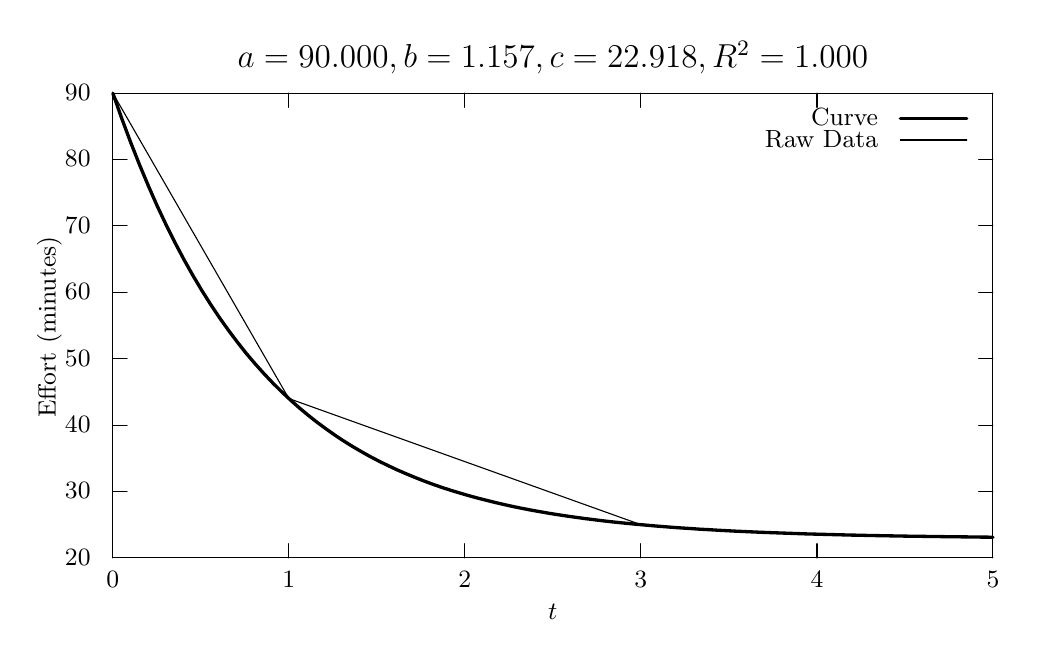
\begin{tikzpicture}[gnuplot]
%% generated with GNUPLOT 4.6p4 (Lua 5.1; terminal rev. 99, script rev. 100)
%% Fri 03 Oct 2014 12:39:55 WST
\tikzset{every node/.append style={font={\fontsize{9pt}{10.8pt}\selectfont}}}
\gpmonochromelines
\path (0.000,0.000) rectangle (12.700,7.620);
\gpcolor{color=gp lt color border}
\gpsetlinetype{gp lt border}
\gpsetlinewidth{1.00}
\draw[gp path] (1.024,0.886)--(1.204,0.886);
\draw[gp path] (12.201,0.886)--(12.021,0.886);
\node[gp node right] at (0.858,0.886) {20};
\draw[gp path] (1.024,1.729)--(1.204,1.729);
\draw[gp path] (12.201,1.729)--(12.021,1.729);
\node[gp node right] at (0.858,1.729) {30};
\draw[gp path] (1.024,2.572)--(1.204,2.572);
\draw[gp path] (12.201,2.572)--(12.021,2.572);
\node[gp node right] at (0.858,2.572) {40};
\draw[gp path] (1.024,3.415)--(1.204,3.415);
\draw[gp path] (12.201,3.415)--(12.021,3.415);
\node[gp node right] at (0.858,3.415) {50};
\draw[gp path] (1.024,4.259)--(1.204,4.259);
\draw[gp path] (12.201,4.259)--(12.021,4.259);
\node[gp node right] at (0.858,4.259) {60};
\draw[gp path] (1.024,5.102)--(1.204,5.102);
\draw[gp path] (12.201,5.102)--(12.021,5.102);
\node[gp node right] at (0.858,5.102) {70};
\draw[gp path] (1.024,5.945)--(1.204,5.945);
\draw[gp path] (12.201,5.945)--(12.021,5.945);
\node[gp node right] at (0.858,5.945) {80};
\draw[gp path] (1.024,6.788)--(1.204,6.788);
\draw[gp path] (12.201,6.788)--(12.021,6.788);
\node[gp node right] at (0.858,6.788) {90};
\draw[gp path] (1.024,0.886)--(1.024,1.066);
\draw[gp path] (1.024,6.788)--(1.024,6.608);
\node[gp node center] at (1.024,0.609) {0};
\draw[gp path] (3.259,0.886)--(3.259,1.066);
\draw[gp path] (3.259,6.788)--(3.259,6.608);
\node[gp node center] at (3.259,0.609) {1};
\draw[gp path] (5.495,0.886)--(5.495,1.066);
\draw[gp path] (5.495,6.788)--(5.495,6.608);
\node[gp node center] at (5.495,0.609) {2};
\draw[gp path] (7.730,0.886)--(7.730,1.066);
\draw[gp path] (7.730,6.788)--(7.730,6.608);
\node[gp node center] at (7.730,0.609) {3};
\draw[gp path] (9.966,0.886)--(9.966,1.066);
\draw[gp path] (9.966,6.788)--(9.966,6.608);
\node[gp node center] at (9.966,0.609) {4};
\draw[gp path] (12.201,0.886)--(12.201,1.066);
\draw[gp path] (12.201,6.788)--(12.201,6.608);
\node[gp node center] at (12.201,0.609) {5};
\draw[gp path] (1.024,6.788)--(1.024,0.886)--(12.201,0.886)--(12.201,6.788)--cycle;
\node[gp node center,rotate=-270] at (0.221,3.837) {Effort (minutes)};
\node[gp node center] at (6.612,0.194) {$t$};
\node[gp node center,font={\fontsize{12pt}{14.4pt}\selectfont}] at (6.612,7.204) {$a = 90.000, b = 1.157, c = 22.918, R^2 = 1.000$};
\node[gp node right] at (10.859,6.470) {Curve};
\gpcolor{color=gp lt color 0}
\gpsetlinetype{gp lt plot 0}
\gpsetlinewidth{3.00}
\draw[gp path] (11.025,6.470)--(11.869,6.470);
\draw[gp path] (1.024,6.788)--(1.137,6.467)--(1.250,6.164)--(1.363,5.878)--(1.476,5.609)%
  --(1.588,5.354)--(1.701,5.115)--(1.814,4.889)--(1.927,4.675)--(2.040,4.474)--(2.153,4.284)%
  --(2.266,4.105)--(2.379,3.936)--(2.492,3.777)--(2.605,3.627)--(2.717,3.485)--(2.830,3.352)%
  --(2.943,3.226)--(3.056,3.107)--(3.169,2.995)--(3.282,2.889)--(3.395,2.789)--(3.508,2.695)%
  --(3.621,2.606)--(3.734,2.523)--(3.846,2.444)--(3.959,2.369)--(4.072,2.299)--(4.185,2.233)%
  --(4.298,2.170)--(4.411,2.111)--(4.524,2.056)--(4.637,2.003)--(4.750,1.954)--(4.863,1.907)%
  --(4.975,1.863)--(5.088,1.821)--(5.201,1.782)--(5.314,1.745)--(5.427,1.711)--(5.540,1.678)%
  --(5.653,1.647)--(5.766,1.618)--(5.879,1.590)--(5.992,1.564)--(6.104,1.539)--(6.217,1.516)%
  --(6.330,1.494)--(6.443,1.474)--(6.556,1.454)--(6.669,1.436)--(6.782,1.419)--(6.895,1.403)%
  --(7.008,1.387)--(7.121,1.373)--(7.233,1.359)--(7.346,1.346)--(7.459,1.334)--(7.572,1.323)%
  --(7.685,1.312)--(7.798,1.302)--(7.911,1.292)--(8.024,1.283)--(8.137,1.274)--(8.250,1.266)%
  --(8.362,1.259)--(8.475,1.251)--(8.588,1.245)--(8.701,1.238)--(8.814,1.232)--(8.927,1.226)%
  --(9.040,1.221)--(9.153,1.216)--(9.266,1.211)--(9.379,1.207)--(9.491,1.203)--(9.604,1.199)%
  --(9.717,1.195)--(9.830,1.191)--(9.943,1.188)--(10.056,1.185)--(10.169,1.182)--(10.282,1.179)%
  --(10.395,1.176)--(10.508,1.174)--(10.620,1.171)--(10.733,1.169)--(10.846,1.167)--(10.959,1.165)%
  --(11.072,1.163)--(11.185,1.161)--(11.298,1.160)--(11.411,1.158)--(11.524,1.157)--(11.637,1.155)%
  --(11.749,1.154)--(11.862,1.153)--(11.975,1.151)--(12.088,1.150)--(12.201,1.149);
\gpcolor{color=gp lt color border}
\node[gp node right] at (10.859,6.193) {Raw Data};
\gpcolor{color=gp lt color 3}
\gpsetlinetype{gp lt plot 3}
\gpsetlinewidth{1.00}
\draw[gp path] (11.025,6.193)--(11.869,6.193);
\draw[gp path] (1.024,6.788)--(3.259,2.910)--(7.730,1.308);
\gpcolor{color=gp lt color border}
\gpsetlinetype{gp lt border}
\draw[gp path] (1.024,6.788)--(1.024,0.886)--(12.201,0.886)--(12.201,6.788)--cycle;
%% coordinates of the plot area
\gpdefrectangularnode{gp plot 1}{\pgfpoint{1.024cm}{0.886cm}}{\pgfpoint{12.201cm}{6.788cm}}
\end{tikzpicture}
%% gnuplot variables

  \caption{$(a-c) e^{-bt} + c$}
  \end{figure}
  
  \begin{figure}[!htb]
  \centering
  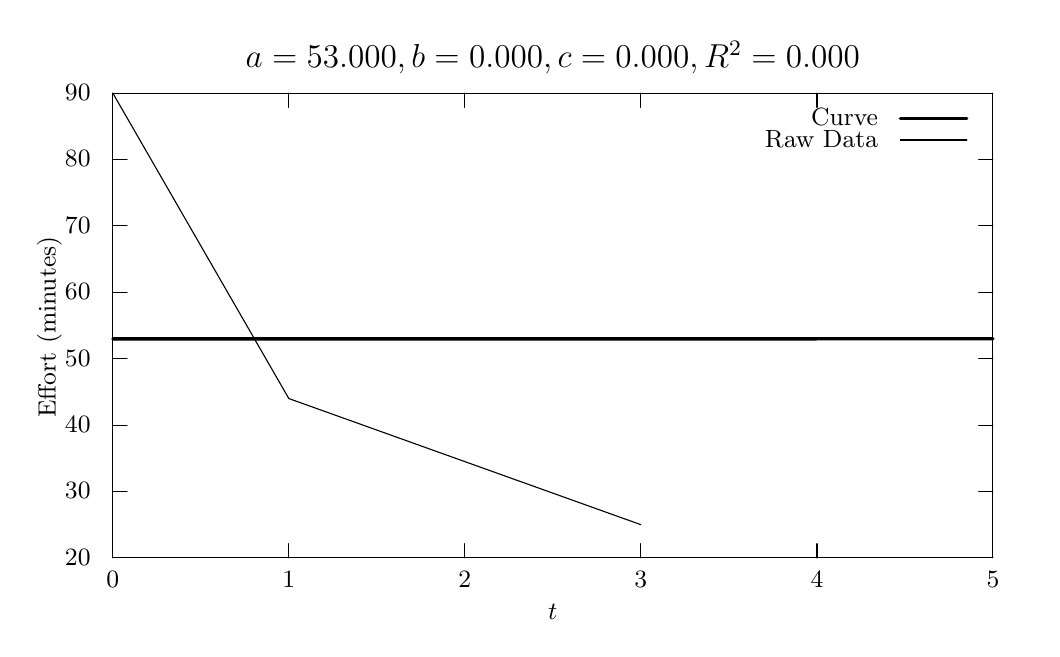
\begin{tikzpicture}[gnuplot]
%% generated with GNUPLOT 4.6p4 (Lua 5.1; terminal rev. 99, script rev. 100)
%% Fri 03 Oct 2014 12:39:55 WST
\tikzset{every node/.append style={font={\fontsize{9pt}{10.8pt}\selectfont}}}
\gpmonochromelines
\path (0.000,0.000) rectangle (12.700,7.620);
\gpcolor{color=gp lt color border}
\gpsetlinetype{gp lt border}
\gpsetlinewidth{1.00}
\draw[gp path] (1.024,0.886)--(1.204,0.886);
\draw[gp path] (12.201,0.886)--(12.021,0.886);
\node[gp node right] at (0.858,0.886) {20};
\draw[gp path] (1.024,1.729)--(1.204,1.729);
\draw[gp path] (12.201,1.729)--(12.021,1.729);
\node[gp node right] at (0.858,1.729) {30};
\draw[gp path] (1.024,2.572)--(1.204,2.572);
\draw[gp path] (12.201,2.572)--(12.021,2.572);
\node[gp node right] at (0.858,2.572) {40};
\draw[gp path] (1.024,3.415)--(1.204,3.415);
\draw[gp path] (12.201,3.415)--(12.021,3.415);
\node[gp node right] at (0.858,3.415) {50};
\draw[gp path] (1.024,4.259)--(1.204,4.259);
\draw[gp path] (12.201,4.259)--(12.021,4.259);
\node[gp node right] at (0.858,4.259) {60};
\draw[gp path] (1.024,5.102)--(1.204,5.102);
\draw[gp path] (12.201,5.102)--(12.021,5.102);
\node[gp node right] at (0.858,5.102) {70};
\draw[gp path] (1.024,5.945)--(1.204,5.945);
\draw[gp path] (12.201,5.945)--(12.021,5.945);
\node[gp node right] at (0.858,5.945) {80};
\draw[gp path] (1.024,6.788)--(1.204,6.788);
\draw[gp path] (12.201,6.788)--(12.021,6.788);
\node[gp node right] at (0.858,6.788) {90};
\draw[gp path] (1.024,0.886)--(1.024,1.066);
\draw[gp path] (1.024,6.788)--(1.024,6.608);
\node[gp node center] at (1.024,0.609) {0};
\draw[gp path] (3.259,0.886)--(3.259,1.066);
\draw[gp path] (3.259,6.788)--(3.259,6.608);
\node[gp node center] at (3.259,0.609) {1};
\draw[gp path] (5.495,0.886)--(5.495,1.066);
\draw[gp path] (5.495,6.788)--(5.495,6.608);
\node[gp node center] at (5.495,0.609) {2};
\draw[gp path] (7.730,0.886)--(7.730,1.066);
\draw[gp path] (7.730,6.788)--(7.730,6.608);
\node[gp node center] at (7.730,0.609) {3};
\draw[gp path] (9.966,0.886)--(9.966,1.066);
\draw[gp path] (9.966,6.788)--(9.966,6.608);
\node[gp node center] at (9.966,0.609) {4};
\draw[gp path] (12.201,0.886)--(12.201,1.066);
\draw[gp path] (12.201,6.788)--(12.201,6.608);
\node[gp node center] at (12.201,0.609) {5};
\draw[gp path] (1.024,6.788)--(1.024,0.886)--(12.201,0.886)--(12.201,6.788)--cycle;
\node[gp node center,rotate=-270] at (0.221,3.837) {Effort (minutes)};
\node[gp node center] at (6.612,0.194) {$t$};
\node[gp node center,font={\fontsize{12pt}{14.4pt}\selectfont}] at (6.612,7.204) {$a = 53.000, b = 0.000, c = 0.000, R^2 = 0.000$};
\node[gp node right] at (10.859,6.470) {Curve};
\gpcolor{color=gp lt color 0}
\gpsetlinetype{gp lt plot 0}
\gpsetlinewidth{3.00}
\draw[gp path] (11.025,6.470)--(11.869,6.470);
\draw[gp path] (1.024,3.668)--(1.137,3.668)--(1.250,3.668)--(1.363,3.668)--(1.476,3.668)%
  --(1.588,3.668)--(1.701,3.668)--(1.814,3.668)--(1.927,3.668)--(2.040,3.668)--(2.153,3.668)%
  --(2.266,3.668)--(2.379,3.668)--(2.492,3.668)--(2.605,3.668)--(2.717,3.668)--(2.830,3.668)%
  --(2.943,3.668)--(3.056,3.668)--(3.169,3.668)--(3.282,3.668)--(3.395,3.668)--(3.508,3.668)%
  --(3.621,3.668)--(3.734,3.668)--(3.846,3.668)--(3.959,3.668)--(4.072,3.668)--(4.185,3.668)%
  --(4.298,3.668)--(4.411,3.668)--(4.524,3.668)--(4.637,3.668)--(4.750,3.668)--(4.863,3.668)%
  --(4.975,3.668)--(5.088,3.668)--(5.201,3.668)--(5.314,3.668)--(5.427,3.668)--(5.540,3.668)%
  --(5.653,3.668)--(5.766,3.668)--(5.879,3.668)--(5.992,3.668)--(6.104,3.668)--(6.217,3.668)%
  --(6.330,3.668)--(6.443,3.668)--(6.556,3.668)--(6.669,3.668)--(6.782,3.668)--(6.895,3.668)%
  --(7.008,3.668)--(7.121,3.668)--(7.233,3.668)--(7.346,3.668)--(7.459,3.668)--(7.572,3.668)%
  --(7.685,3.668)--(7.798,3.668)--(7.911,3.668)--(8.024,3.668)--(8.137,3.668)--(8.250,3.668)%
  --(8.362,3.668)--(8.475,3.668)--(8.588,3.668)--(8.701,3.668)--(8.814,3.668)--(8.927,3.668)%
  --(9.040,3.668)--(9.153,3.668)--(9.266,3.668)--(9.379,3.668)--(9.491,3.668)--(9.604,3.668)%
  --(9.717,3.668)--(9.830,3.668)--(9.943,3.668)--(10.056,3.669)--(10.169,3.669)--(10.282,3.669)%
  --(10.395,3.669)--(10.508,3.669)--(10.620,3.669)--(10.733,3.669)--(10.846,3.669)--(10.959,3.669)%
  --(11.072,3.669)--(11.185,3.669)--(11.298,3.669)--(11.411,3.669)--(11.524,3.669)--(11.637,3.669)%
  --(11.749,3.669)--(11.862,3.669)--(11.975,3.669)--(12.088,3.669)--(12.201,3.669);
\gpcolor{color=gp lt color border}
\node[gp node right] at (10.859,6.193) {Raw Data};
\gpcolor{color=gp lt color 3}
\gpsetlinetype{gp lt plot 3}
\gpsetlinewidth{1.00}
\draw[gp path] (11.025,6.193)--(11.869,6.193);
\draw[gp path] (1.024,6.788)--(3.259,2.910)--(7.730,1.308);
\gpcolor{color=gp lt color border}
\gpsetlinetype{gp lt border}
\draw[gp path] (1.024,6.788)--(1.024,0.886)--(12.201,0.886)--(12.201,6.788)--cycle;
%% coordinates of the plot area
\gpdefrectangularnode{gp plot 1}{\pgfpoint{1.024cm}{0.886cm}}{\pgfpoint{12.201cm}{6.788cm}}
\end{tikzpicture}
%% gnuplot variables

  \caption{$a+bt+ct^2$}
  \end{figure}
  
  \clearpage
  \subsection{Including Outlier}
  \label{subsec:inclout}
  
  Note: These graphs do not meet specified fitting constraints.
  
  \begin{figure}[!htb]
  \centering
  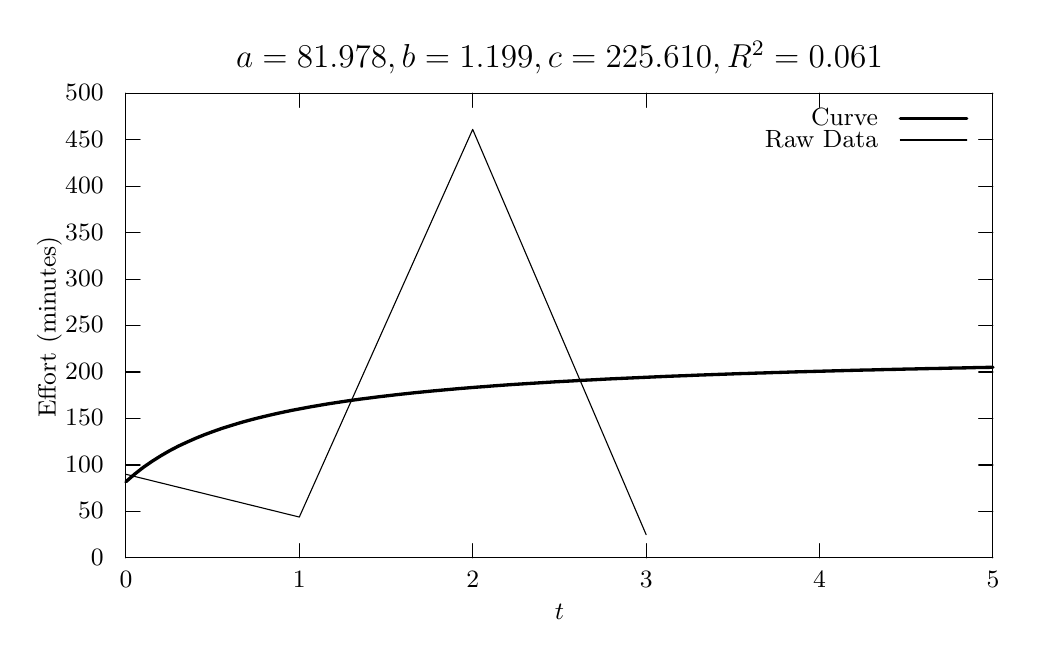
\begin{tikzpicture}[gnuplot]
%% generated with GNUPLOT 4.6p4 (Lua 5.1; terminal rev. 99, script rev. 100)
%% Fri 03 Oct 2014 12:39:55 WST
\tikzset{every node/.append style={font={\fontsize{9pt}{10.8pt}\selectfont}}}
\gpmonochromelines
\path (0.000,0.000) rectangle (12.700,7.620);
\gpcolor{color=gp lt color border}
\gpsetlinetype{gp lt border}
\gpsetlinewidth{1.00}
\draw[gp path] (1.190,0.886)--(1.370,0.886);
\draw[gp path] (12.201,0.886)--(12.021,0.886);
\node[gp node right] at (1.024,0.886) {0};
\draw[gp path] (1.190,1.476)--(1.370,1.476);
\draw[gp path] (12.201,1.476)--(12.021,1.476);
\node[gp node right] at (1.024,1.476) {50};
\draw[gp path] (1.190,2.066)--(1.370,2.066);
\draw[gp path] (12.201,2.066)--(12.021,2.066);
\node[gp node right] at (1.024,2.066) {100};
\draw[gp path] (1.190,2.657)--(1.370,2.657);
\draw[gp path] (12.201,2.657)--(12.021,2.657);
\node[gp node right] at (1.024,2.657) {150};
\draw[gp path] (1.190,3.247)--(1.370,3.247);
\draw[gp path] (12.201,3.247)--(12.021,3.247);
\node[gp node right] at (1.024,3.247) {200};
\draw[gp path] (1.190,3.837)--(1.370,3.837);
\draw[gp path] (12.201,3.837)--(12.021,3.837);
\node[gp node right] at (1.024,3.837) {250};
\draw[gp path] (1.190,4.427)--(1.370,4.427);
\draw[gp path] (12.201,4.427)--(12.021,4.427);
\node[gp node right] at (1.024,4.427) {300};
\draw[gp path] (1.190,5.017)--(1.370,5.017);
\draw[gp path] (12.201,5.017)--(12.021,5.017);
\node[gp node right] at (1.024,5.017) {350};
\draw[gp path] (1.190,5.608)--(1.370,5.608);
\draw[gp path] (12.201,5.608)--(12.021,5.608);
\node[gp node right] at (1.024,5.608) {400};
\draw[gp path] (1.190,6.198)--(1.370,6.198);
\draw[gp path] (12.201,6.198)--(12.021,6.198);
\node[gp node right] at (1.024,6.198) {450};
\draw[gp path] (1.190,6.788)--(1.370,6.788);
\draw[gp path] (12.201,6.788)--(12.021,6.788);
\node[gp node right] at (1.024,6.788) {500};
\draw[gp path] (1.190,0.886)--(1.190,1.066);
\draw[gp path] (1.190,6.788)--(1.190,6.608);
\node[gp node center] at (1.190,0.609) {0};
\draw[gp path] (3.392,0.886)--(3.392,1.066);
\draw[gp path] (3.392,6.788)--(3.392,6.608);
\node[gp node center] at (3.392,0.609) {1};
\draw[gp path] (5.594,0.886)--(5.594,1.066);
\draw[gp path] (5.594,6.788)--(5.594,6.608);
\node[gp node center] at (5.594,0.609) {2};
\draw[gp path] (7.797,0.886)--(7.797,1.066);
\draw[gp path] (7.797,6.788)--(7.797,6.608);
\node[gp node center] at (7.797,0.609) {3};
\draw[gp path] (9.999,0.886)--(9.999,1.066);
\draw[gp path] (9.999,6.788)--(9.999,6.608);
\node[gp node center] at (9.999,0.609) {4};
\draw[gp path] (12.201,0.886)--(12.201,1.066);
\draw[gp path] (12.201,6.788)--(12.201,6.608);
\node[gp node center] at (12.201,0.609) {5};
\draw[gp path] (1.190,6.788)--(1.190,0.886)--(12.201,0.886)--(12.201,6.788)--cycle;
\node[gp node center,rotate=-270] at (0.221,3.837) {Effort (minutes)};
\node[gp node center] at (6.695,0.194) {$t$};
\node[gp node center,font={\fontsize{12pt}{14.4pt}\selectfont}] at (6.695,7.204) {$a = 81.978, b = 1.199, c = 225.610, R^2 = 0.061$};
\node[gp node right] at (10.859,6.470) {Curve};
\gpcolor{color=gp lt color 0}
\gpsetlinetype{gp lt plot 0}
\gpsetlinewidth{3.00}
\draw[gp path] (11.025,6.470)--(11.869,6.470);
\draw[gp path] (1.190,1.854)--(1.301,1.950)--(1.412,2.037)--(1.524,2.114)--(1.635,2.184)%
  --(1.746,2.248)--(1.857,2.306)--(1.969,2.358)--(2.080,2.407)--(2.191,2.452)--(2.302,2.493)%
  --(2.413,2.532)--(2.525,2.567)--(2.636,2.601)--(2.747,2.632)--(2.858,2.661)--(2.970,2.688)%
  --(3.081,2.714)--(3.192,2.738)--(3.303,2.761)--(3.414,2.782)--(3.526,2.803)--(3.637,2.822)%
  --(3.748,2.841)--(3.859,2.858)--(3.971,2.875)--(4.082,2.891)--(4.193,2.906)--(4.304,2.920)%
  --(4.415,2.934)--(4.527,2.947)--(4.638,2.960)--(4.749,2.972)--(4.860,2.984)--(4.972,2.995)%
  --(5.083,3.006)--(5.194,3.016)--(5.305,3.026)--(5.416,3.036)--(5.528,3.045)--(5.639,3.054)%
  --(5.750,3.062)--(5.861,3.071)--(5.973,3.079)--(6.084,3.087)--(6.195,3.094)--(6.306,3.101)%
  --(6.417,3.108)--(6.529,3.115)--(6.640,3.122)--(6.751,3.128)--(6.862,3.134)--(6.974,3.141)%
  --(7.085,3.146)--(7.196,3.152)--(7.307,3.158)--(7.418,3.163)--(7.530,3.168)--(7.641,3.173)%
  --(7.752,3.178)--(7.863,3.183)--(7.975,3.188)--(8.086,3.193)--(8.197,3.197)--(8.308,3.201)%
  --(8.419,3.206)--(8.531,3.210)--(8.642,3.214)--(8.753,3.218)--(8.864,3.222)--(8.976,3.226)%
  --(9.087,3.229)--(9.198,3.233)--(9.309,3.236)--(9.420,3.240)--(9.532,3.243)--(9.643,3.247)%
  --(9.754,3.250)--(9.865,3.253)--(9.977,3.256)--(10.088,3.259)--(10.199,3.262)--(10.310,3.265)%
  --(10.421,3.268)--(10.533,3.271)--(10.644,3.273)--(10.755,3.276)--(10.866,3.279)--(10.978,3.281)%
  --(11.089,3.284)--(11.200,3.286)--(11.311,3.289)--(11.422,3.291)--(11.534,3.293)--(11.645,3.296)%
  --(11.756,3.298)--(11.867,3.300)--(11.979,3.303)--(12.090,3.305)--(12.201,3.307);
\gpcolor{color=gp lt color border}
\node[gp node right] at (10.859,6.193) {Raw Data};
\gpcolor{color=gp lt color 3}
\gpsetlinetype{gp lt plot 3}
\gpsetlinewidth{1.00}
\draw[gp path] (11.025,6.193)--(11.869,6.193);
\draw[gp path] (1.190,1.948)--(3.392,1.405)--(5.594,6.328)--(7.797,1.181);
\gpcolor{color=gp lt color border}
\gpsetlinetype{gp lt border}
\draw[gp path] (1.190,6.788)--(1.190,0.886)--(12.201,0.886)--(12.201,6.788)--cycle;
%% coordinates of the plot area
\gpdefrectangularnode{gp plot 1}{\pgfpoint{1.190cm}{0.886cm}}{\pgfpoint{12.201cm}{6.788cm}}
\end{tikzpicture}
%% gnuplot variables

  \caption{$\frac{a+bct}{bt+1}$}
  \end{figure}
  
  \begin{figure}[!htb]
  \centering
  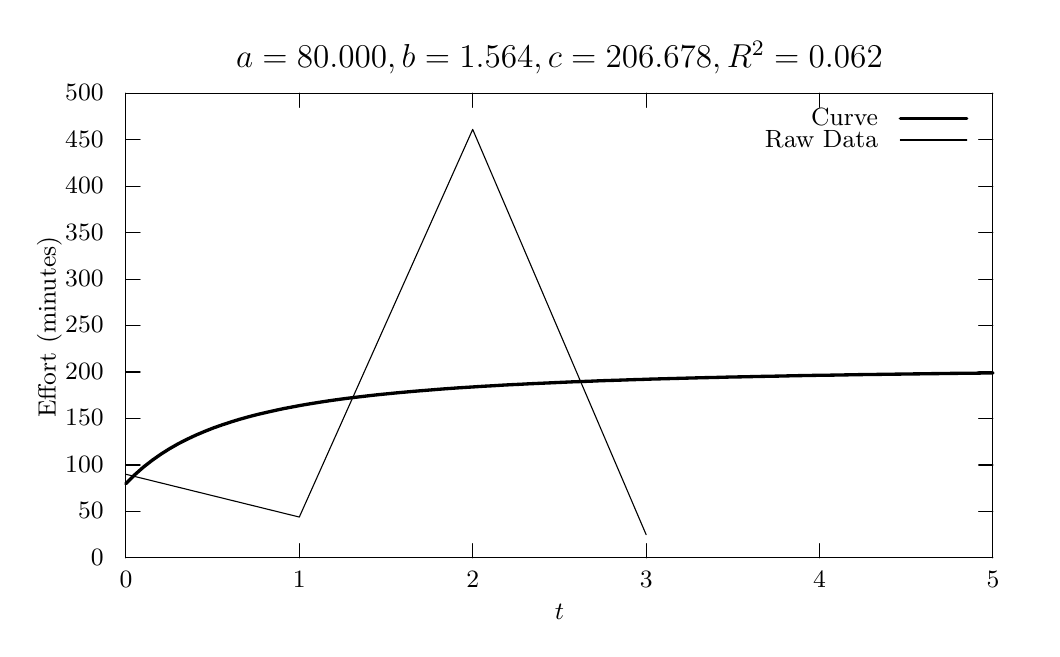
\begin{tikzpicture}[gnuplot]
%% generated with GNUPLOT 4.6p4 (Lua 5.1; terminal rev. 99, script rev. 100)
%% Fri 03 Oct 2014 12:39:55 WST
\tikzset{every node/.append style={font={\fontsize{9pt}{10.8pt}\selectfont}}}
\gpmonochromelines
\path (0.000,0.000) rectangle (12.700,7.620);
\gpcolor{color=gp lt color border}
\gpsetlinetype{gp lt border}
\gpsetlinewidth{1.00}
\draw[gp path] (1.190,0.886)--(1.370,0.886);
\draw[gp path] (12.201,0.886)--(12.021,0.886);
\node[gp node right] at (1.024,0.886) {0};
\draw[gp path] (1.190,1.476)--(1.370,1.476);
\draw[gp path] (12.201,1.476)--(12.021,1.476);
\node[gp node right] at (1.024,1.476) {50};
\draw[gp path] (1.190,2.066)--(1.370,2.066);
\draw[gp path] (12.201,2.066)--(12.021,2.066);
\node[gp node right] at (1.024,2.066) {100};
\draw[gp path] (1.190,2.657)--(1.370,2.657);
\draw[gp path] (12.201,2.657)--(12.021,2.657);
\node[gp node right] at (1.024,2.657) {150};
\draw[gp path] (1.190,3.247)--(1.370,3.247);
\draw[gp path] (12.201,3.247)--(12.021,3.247);
\node[gp node right] at (1.024,3.247) {200};
\draw[gp path] (1.190,3.837)--(1.370,3.837);
\draw[gp path] (12.201,3.837)--(12.021,3.837);
\node[gp node right] at (1.024,3.837) {250};
\draw[gp path] (1.190,4.427)--(1.370,4.427);
\draw[gp path] (12.201,4.427)--(12.021,4.427);
\node[gp node right] at (1.024,4.427) {300};
\draw[gp path] (1.190,5.017)--(1.370,5.017);
\draw[gp path] (12.201,5.017)--(12.021,5.017);
\node[gp node right] at (1.024,5.017) {350};
\draw[gp path] (1.190,5.608)--(1.370,5.608);
\draw[gp path] (12.201,5.608)--(12.021,5.608);
\node[gp node right] at (1.024,5.608) {400};
\draw[gp path] (1.190,6.198)--(1.370,6.198);
\draw[gp path] (12.201,6.198)--(12.021,6.198);
\node[gp node right] at (1.024,6.198) {450};
\draw[gp path] (1.190,6.788)--(1.370,6.788);
\draw[gp path] (12.201,6.788)--(12.021,6.788);
\node[gp node right] at (1.024,6.788) {500};
\draw[gp path] (1.190,0.886)--(1.190,1.066);
\draw[gp path] (1.190,6.788)--(1.190,6.608);
\node[gp node center] at (1.190,0.609) {0};
\draw[gp path] (3.392,0.886)--(3.392,1.066);
\draw[gp path] (3.392,6.788)--(3.392,6.608);
\node[gp node center] at (3.392,0.609) {1};
\draw[gp path] (5.594,0.886)--(5.594,1.066);
\draw[gp path] (5.594,6.788)--(5.594,6.608);
\node[gp node center] at (5.594,0.609) {2};
\draw[gp path] (7.797,0.886)--(7.797,1.066);
\draw[gp path] (7.797,6.788)--(7.797,6.608);
\node[gp node center] at (7.797,0.609) {3};
\draw[gp path] (9.999,0.886)--(9.999,1.066);
\draw[gp path] (9.999,6.788)--(9.999,6.608);
\node[gp node center] at (9.999,0.609) {4};
\draw[gp path] (12.201,0.886)--(12.201,1.066);
\draw[gp path] (12.201,6.788)--(12.201,6.608);
\node[gp node center] at (12.201,0.609) {5};
\draw[gp path] (1.190,6.788)--(1.190,0.886)--(12.201,0.886)--(12.201,6.788)--cycle;
\node[gp node center,rotate=-270] at (0.221,3.837) {Effort (minutes)};
\node[gp node center] at (6.695,0.194) {$t$};
\node[gp node center,font={\fontsize{12pt}{14.4pt}\selectfont}] at (6.695,7.204) {$a = 80.000, b = 1.564, c = 206.678, R^2 = 0.062$};
\node[gp node right] at (10.859,6.470) {Curve};
\gpcolor{color=gp lt color 0}
\gpsetlinetype{gp lt plot 0}
\gpsetlinewidth{3.00}
\draw[gp path] (11.025,6.470)--(11.869,6.470);
\draw[gp path] (1.190,1.830)--(1.301,1.941)--(1.412,2.039)--(1.524,2.126)--(1.635,2.204)%
  --(1.746,2.274)--(1.857,2.337)--(1.969,2.394)--(2.080,2.446)--(2.191,2.493)--(2.302,2.537)%
  --(2.413,2.576)--(2.525,2.613)--(2.636,2.647)--(2.747,2.678)--(2.858,2.707)--(2.970,2.733)%
  --(3.081,2.758)--(3.192,2.782)--(3.303,2.803)--(3.414,2.824)--(3.526,2.843)--(3.637,2.861)%
  --(3.748,2.878)--(3.859,2.894)--(3.971,2.909)--(4.082,2.923)--(4.193,2.936)--(4.304,2.949)%
  --(4.415,2.961)--(4.527,2.972)--(4.638,2.983)--(4.749,2.993)--(4.860,3.003)--(4.972,3.012)%
  --(5.083,3.021)--(5.194,3.030)--(5.305,3.038)--(5.416,3.046)--(5.528,3.053)--(5.639,3.060)%
  --(5.750,3.067)--(5.861,3.073)--(5.973,3.080)--(6.084,3.086)--(6.195,3.091)--(6.306,3.097)%
  --(6.417,3.102)--(6.529,3.107)--(6.640,3.112)--(6.751,3.117)--(6.862,3.122)--(6.974,3.126)%
  --(7.085,3.130)--(7.196,3.135)--(7.307,3.139)--(7.418,3.142)--(7.530,3.146)--(7.641,3.150)%
  --(7.752,3.153)--(7.863,3.157)--(7.975,3.160)--(8.086,3.163)--(8.197,3.166)--(8.308,3.169)%
  --(8.419,3.172)--(8.531,3.175)--(8.642,3.177)--(8.753,3.180)--(8.864,3.183)--(8.976,3.185)%
  --(9.087,3.187)--(9.198,3.190)--(9.309,3.192)--(9.420,3.194)--(9.532,3.196)--(9.643,3.199)%
  --(9.754,3.201)--(9.865,3.203)--(9.977,3.205)--(10.088,3.206)--(10.199,3.208)--(10.310,3.210)%
  --(10.421,3.212)--(10.533,3.214)--(10.644,3.215)--(10.755,3.217)--(10.866,3.218)--(10.978,3.220)%
  --(11.089,3.221)--(11.200,3.223)--(11.311,3.224)--(11.422,3.226)--(11.534,3.227)--(11.645,3.229)%
  --(11.756,3.230)--(11.867,3.231)--(11.979,3.232)--(12.090,3.234)--(12.201,3.235);
\gpcolor{color=gp lt color border}
\node[gp node right] at (10.859,6.193) {Raw Data};
\gpcolor{color=gp lt color 3}
\gpsetlinetype{gp lt plot 3}
\gpsetlinewidth{1.00}
\draw[gp path] (11.025,6.193)--(11.869,6.193);
\draw[gp path] (1.190,1.948)--(3.392,1.405)--(5.594,6.328)--(7.797,1.181);
\gpcolor{color=gp lt color border}
\gpsetlinetype{gp lt border}
\draw[gp path] (1.190,6.788)--(1.190,0.886)--(12.201,0.886)--(12.201,6.788)--cycle;
%% coordinates of the plot area
\gpdefrectangularnode{gp plot 1}{\pgfpoint{1.190cm}{0.886cm}}{\pgfpoint{12.201cm}{6.788cm}}
\end{tikzpicture}
%% gnuplot variables

  \caption{$(a-c)(t+1)^{-b}+c$}
  \end{figure}
  
  \begin{figure}[!htb]
  \centering
  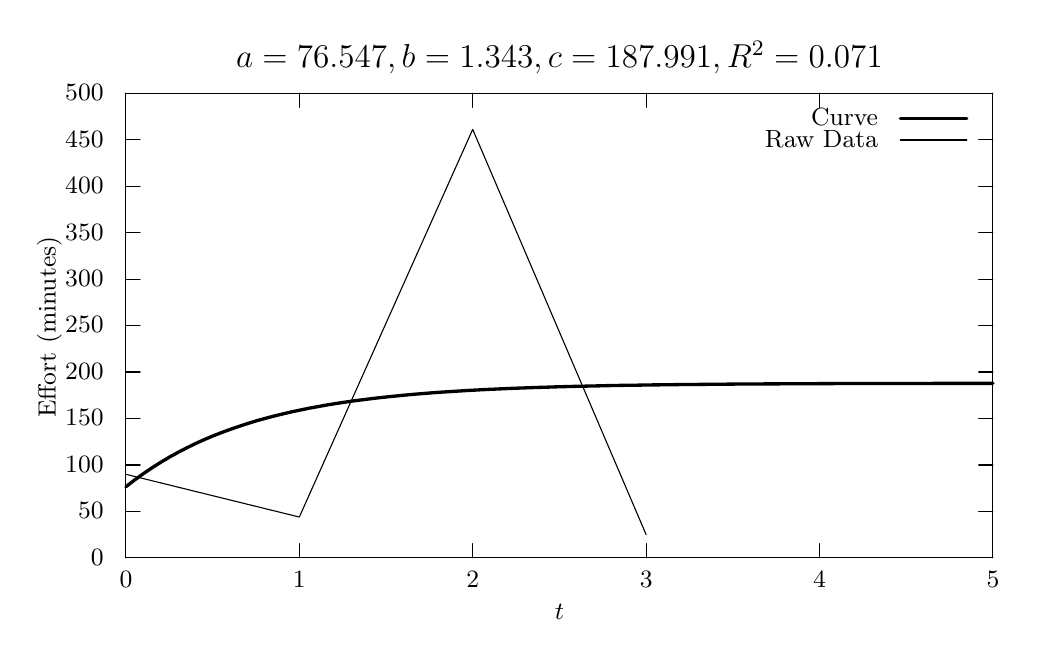
\begin{tikzpicture}[gnuplot]
%% generated with GNUPLOT 4.6p4 (Lua 5.1; terminal rev. 99, script rev. 100)
%% Fri 03 Oct 2014 12:39:55 WST
\tikzset{every node/.append style={font={\fontsize{9pt}{10.8pt}\selectfont}}}
\gpmonochromelines
\path (0.000,0.000) rectangle (12.700,7.620);
\gpcolor{color=gp lt color border}
\gpsetlinetype{gp lt border}
\gpsetlinewidth{1.00}
\draw[gp path] (1.190,0.886)--(1.370,0.886);
\draw[gp path] (12.201,0.886)--(12.021,0.886);
\node[gp node right] at (1.024,0.886) {0};
\draw[gp path] (1.190,1.476)--(1.370,1.476);
\draw[gp path] (12.201,1.476)--(12.021,1.476);
\node[gp node right] at (1.024,1.476) {50};
\draw[gp path] (1.190,2.066)--(1.370,2.066);
\draw[gp path] (12.201,2.066)--(12.021,2.066);
\node[gp node right] at (1.024,2.066) {100};
\draw[gp path] (1.190,2.657)--(1.370,2.657);
\draw[gp path] (12.201,2.657)--(12.021,2.657);
\node[gp node right] at (1.024,2.657) {150};
\draw[gp path] (1.190,3.247)--(1.370,3.247);
\draw[gp path] (12.201,3.247)--(12.021,3.247);
\node[gp node right] at (1.024,3.247) {200};
\draw[gp path] (1.190,3.837)--(1.370,3.837);
\draw[gp path] (12.201,3.837)--(12.021,3.837);
\node[gp node right] at (1.024,3.837) {250};
\draw[gp path] (1.190,4.427)--(1.370,4.427);
\draw[gp path] (12.201,4.427)--(12.021,4.427);
\node[gp node right] at (1.024,4.427) {300};
\draw[gp path] (1.190,5.017)--(1.370,5.017);
\draw[gp path] (12.201,5.017)--(12.021,5.017);
\node[gp node right] at (1.024,5.017) {350};
\draw[gp path] (1.190,5.608)--(1.370,5.608);
\draw[gp path] (12.201,5.608)--(12.021,5.608);
\node[gp node right] at (1.024,5.608) {400};
\draw[gp path] (1.190,6.198)--(1.370,6.198);
\draw[gp path] (12.201,6.198)--(12.021,6.198);
\node[gp node right] at (1.024,6.198) {450};
\draw[gp path] (1.190,6.788)--(1.370,6.788);
\draw[gp path] (12.201,6.788)--(12.021,6.788);
\node[gp node right] at (1.024,6.788) {500};
\draw[gp path] (1.190,0.886)--(1.190,1.066);
\draw[gp path] (1.190,6.788)--(1.190,6.608);
\node[gp node center] at (1.190,0.609) {0};
\draw[gp path] (3.392,0.886)--(3.392,1.066);
\draw[gp path] (3.392,6.788)--(3.392,6.608);
\node[gp node center] at (3.392,0.609) {1};
\draw[gp path] (5.594,0.886)--(5.594,1.066);
\draw[gp path] (5.594,6.788)--(5.594,6.608);
\node[gp node center] at (5.594,0.609) {2};
\draw[gp path] (7.797,0.886)--(7.797,1.066);
\draw[gp path] (7.797,6.788)--(7.797,6.608);
\node[gp node center] at (7.797,0.609) {3};
\draw[gp path] (9.999,0.886)--(9.999,1.066);
\draw[gp path] (9.999,6.788)--(9.999,6.608);
\node[gp node center] at (9.999,0.609) {4};
\draw[gp path] (12.201,0.886)--(12.201,1.066);
\draw[gp path] (12.201,6.788)--(12.201,6.608);
\node[gp node center] at (12.201,0.609) {5};
\draw[gp path] (1.190,6.788)--(1.190,0.886)--(12.201,0.886)--(12.201,6.788)--cycle;
\node[gp node center,rotate=-270] at (0.221,3.837) {Effort (minutes)};
\node[gp node center] at (6.695,0.194) {$t$};
\node[gp node center,font={\fontsize{12pt}{14.4pt}\selectfont}] at (6.695,7.204) {$a = 76.547, b = 1.343, c = 187.991, R^2 = 0.071$};
\node[gp node right] at (10.859,6.470) {Curve};
\gpcolor{color=gp lt color 0}
\gpsetlinetype{gp lt plot 0}
\gpsetlinewidth{3.00}
\draw[gp path] (11.025,6.470)--(11.869,6.470);
\draw[gp path] (1.190,1.790)--(1.301,1.876)--(1.412,1.956)--(1.524,2.032)--(1.635,2.102)%
  --(1.746,2.168)--(1.857,2.229)--(1.969,2.287)--(2.080,2.341)--(2.191,2.391)--(2.302,2.438)%
  --(2.413,2.481)--(2.525,2.522)--(2.636,2.560)--(2.747,2.596)--(2.858,2.630)--(2.970,2.661)%
  --(3.081,2.690)--(3.192,2.717)--(3.303,2.743)--(3.414,2.766)--(3.526,2.789)--(3.637,2.809)%
  --(3.748,2.829)--(3.859,2.847)--(3.971,2.864)--(4.082,2.880)--(4.193,2.894)--(4.304,2.908)%
  --(4.415,2.921)--(4.527,2.933)--(4.638,2.944)--(4.749,2.955)--(4.860,2.965)--(4.972,2.974)%
  --(5.083,2.983)--(5.194,2.991)--(5.305,2.998)--(5.416,3.005)--(5.528,3.012)--(5.639,3.018)%
  --(5.750,3.024)--(5.861,3.029)--(5.973,3.034)--(6.084,3.039)--(6.195,3.043)--(6.306,3.047)%
  --(6.417,3.051)--(6.529,3.054)--(6.640,3.058)--(6.751,3.061)--(6.862,3.064)--(6.974,3.066)%
  --(7.085,3.069)--(7.196,3.071)--(7.307,3.074)--(7.418,3.076)--(7.530,3.078)--(7.641,3.079)%
  --(7.752,3.081)--(7.863,3.083)--(7.975,3.084)--(8.086,3.085)--(8.197,3.087)--(8.308,3.088)%
  --(8.419,3.089)--(8.531,3.090)--(8.642,3.091)--(8.753,3.092)--(8.864,3.093)--(8.976,3.094)%
  --(9.087,3.094)--(9.198,3.095)--(9.309,3.096)--(9.420,3.096)--(9.532,3.097)--(9.643,3.097)%
  --(9.754,3.098)--(9.865,3.098)--(9.977,3.099)--(10.088,3.099)--(10.199,3.100)--(10.310,3.100)%
  --(10.421,3.100)--(10.533,3.101)--(10.644,3.101)--(10.755,3.101)--(10.866,3.101)--(10.978,3.102)%
  --(11.089,3.102)--(11.200,3.102)--(11.311,3.102)--(11.422,3.102)--(11.534,3.103)--(11.645,3.103)%
  --(11.756,3.103)--(11.867,3.103)--(11.979,3.103)--(12.090,3.103)--(12.201,3.103);
\gpcolor{color=gp lt color border}
\node[gp node right] at (10.859,6.193) {Raw Data};
\gpcolor{color=gp lt color 3}
\gpsetlinetype{gp lt plot 3}
\gpsetlinewidth{1.00}
\draw[gp path] (11.025,6.193)--(11.869,6.193);
\draw[gp path] (1.190,1.948)--(3.392,1.405)--(5.594,6.328)--(7.797,1.181);
\gpcolor{color=gp lt color border}
\gpsetlinetype{gp lt border}
\draw[gp path] (1.190,6.788)--(1.190,0.886)--(12.201,0.886)--(12.201,6.788)--cycle;
%% coordinates of the plot area
\gpdefrectangularnode{gp plot 1}{\pgfpoint{1.190cm}{0.886cm}}{\pgfpoint{12.201cm}{6.788cm}}
\end{tikzpicture}
%% gnuplot variables

  \caption{$(a-c) e^{-bt} + c$}
  \end{figure}
  
  \begin{figure}[!htb]
  \centering
  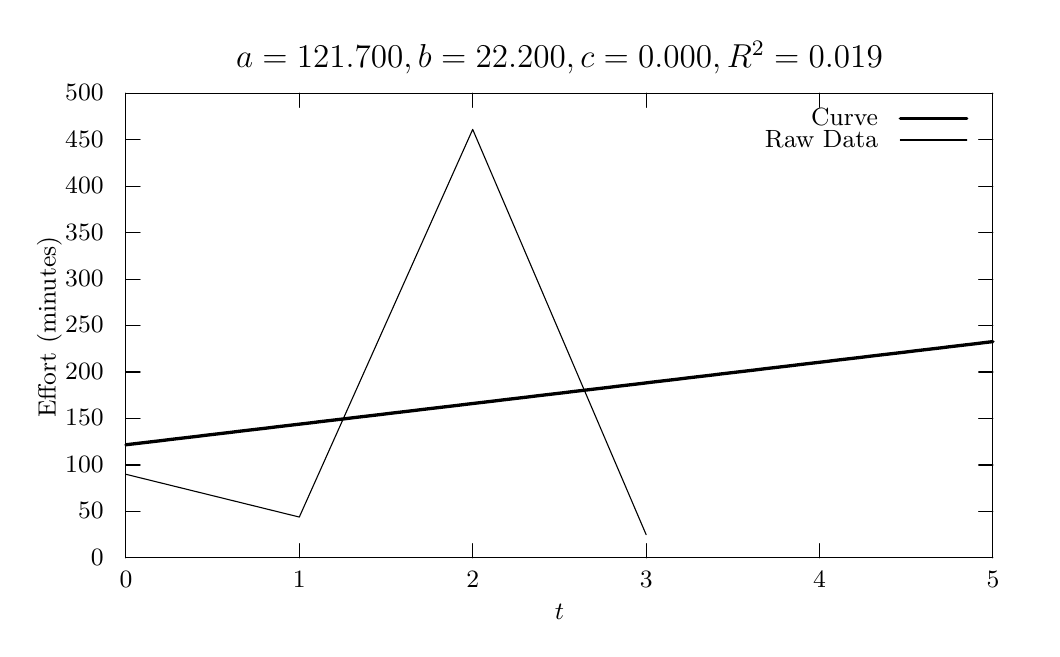
\begin{tikzpicture}[gnuplot]
%% generated with GNUPLOT 4.6p4 (Lua 5.1; terminal rev. 99, script rev. 100)
%% Fri 03 Oct 2014 12:39:55 WST
\tikzset{every node/.append style={font={\fontsize{9pt}{10.8pt}\selectfont}}}
\gpmonochromelines
\path (0.000,0.000) rectangle (12.700,7.620);
\gpcolor{color=gp lt color border}
\gpsetlinetype{gp lt border}
\gpsetlinewidth{1.00}
\draw[gp path] (1.190,0.886)--(1.370,0.886);
\draw[gp path] (12.201,0.886)--(12.021,0.886);
\node[gp node right] at (1.024,0.886) {0};
\draw[gp path] (1.190,1.476)--(1.370,1.476);
\draw[gp path] (12.201,1.476)--(12.021,1.476);
\node[gp node right] at (1.024,1.476) {50};
\draw[gp path] (1.190,2.066)--(1.370,2.066);
\draw[gp path] (12.201,2.066)--(12.021,2.066);
\node[gp node right] at (1.024,2.066) {100};
\draw[gp path] (1.190,2.657)--(1.370,2.657);
\draw[gp path] (12.201,2.657)--(12.021,2.657);
\node[gp node right] at (1.024,2.657) {150};
\draw[gp path] (1.190,3.247)--(1.370,3.247);
\draw[gp path] (12.201,3.247)--(12.021,3.247);
\node[gp node right] at (1.024,3.247) {200};
\draw[gp path] (1.190,3.837)--(1.370,3.837);
\draw[gp path] (12.201,3.837)--(12.021,3.837);
\node[gp node right] at (1.024,3.837) {250};
\draw[gp path] (1.190,4.427)--(1.370,4.427);
\draw[gp path] (12.201,4.427)--(12.021,4.427);
\node[gp node right] at (1.024,4.427) {300};
\draw[gp path] (1.190,5.017)--(1.370,5.017);
\draw[gp path] (12.201,5.017)--(12.021,5.017);
\node[gp node right] at (1.024,5.017) {350};
\draw[gp path] (1.190,5.608)--(1.370,5.608);
\draw[gp path] (12.201,5.608)--(12.021,5.608);
\node[gp node right] at (1.024,5.608) {400};
\draw[gp path] (1.190,6.198)--(1.370,6.198);
\draw[gp path] (12.201,6.198)--(12.021,6.198);
\node[gp node right] at (1.024,6.198) {450};
\draw[gp path] (1.190,6.788)--(1.370,6.788);
\draw[gp path] (12.201,6.788)--(12.021,6.788);
\node[gp node right] at (1.024,6.788) {500};
\draw[gp path] (1.190,0.886)--(1.190,1.066);
\draw[gp path] (1.190,6.788)--(1.190,6.608);
\node[gp node center] at (1.190,0.609) {0};
\draw[gp path] (3.392,0.886)--(3.392,1.066);
\draw[gp path] (3.392,6.788)--(3.392,6.608);
\node[gp node center] at (3.392,0.609) {1};
\draw[gp path] (5.594,0.886)--(5.594,1.066);
\draw[gp path] (5.594,6.788)--(5.594,6.608);
\node[gp node center] at (5.594,0.609) {2};
\draw[gp path] (7.797,0.886)--(7.797,1.066);
\draw[gp path] (7.797,6.788)--(7.797,6.608);
\node[gp node center] at (7.797,0.609) {3};
\draw[gp path] (9.999,0.886)--(9.999,1.066);
\draw[gp path] (9.999,6.788)--(9.999,6.608);
\node[gp node center] at (9.999,0.609) {4};
\draw[gp path] (12.201,0.886)--(12.201,1.066);
\draw[gp path] (12.201,6.788)--(12.201,6.608);
\node[gp node center] at (12.201,0.609) {5};
\draw[gp path] (1.190,6.788)--(1.190,0.886)--(12.201,0.886)--(12.201,6.788)--cycle;
\node[gp node center,rotate=-270] at (0.221,3.837) {Effort (minutes)};
\node[gp node center] at (6.695,0.194) {$t$};
\node[gp node center,font={\fontsize{12pt}{14.4pt}\selectfont}] at (6.695,7.204) {$a = 121.700, b = 22.200, c = 0.000, R^2 = 0.019$};
\node[gp node right] at (10.859,6.470) {Curve};
\gpcolor{color=gp lt color 0}
\gpsetlinetype{gp lt plot 0}
\gpsetlinewidth{3.00}
\draw[gp path] (11.025,6.470)--(11.869,6.470);
\draw[gp path] (1.190,2.323)--(1.301,2.336)--(1.412,2.349)--(1.524,2.362)--(1.635,2.375)%
  --(1.746,2.389)--(1.857,2.402)--(1.969,2.415)--(2.080,2.428)--(2.191,2.442)--(2.302,2.455)%
  --(2.413,2.468)--(2.525,2.481)--(2.636,2.495)--(2.747,2.508)--(2.858,2.521)--(2.970,2.534)%
  --(3.081,2.548)--(3.192,2.561)--(3.303,2.574)--(3.414,2.587)--(3.526,2.600)--(3.637,2.614)%
  --(3.748,2.627)--(3.859,2.640)--(3.971,2.653)--(4.082,2.667)--(4.193,2.680)--(4.304,2.693)%
  --(4.415,2.706)--(4.527,2.720)--(4.638,2.733)--(4.749,2.746)--(4.860,2.759)--(4.972,2.773)%
  --(5.083,2.786)--(5.194,2.799)--(5.305,2.812)--(5.416,2.825)--(5.528,2.839)--(5.639,2.852)%
  --(5.750,2.865)--(5.861,2.878)--(5.973,2.892)--(6.084,2.905)--(6.195,2.918)--(6.306,2.931)%
  --(6.417,2.945)--(6.529,2.958)--(6.640,2.971)--(6.751,2.984)--(6.862,2.998)--(6.974,3.011)%
  --(7.085,3.024)--(7.196,3.037)--(7.307,3.050)--(7.418,3.064)--(7.530,3.077)--(7.641,3.090)%
  --(7.752,3.103)--(7.863,3.117)--(7.975,3.130)--(8.086,3.143)--(8.197,3.156)--(8.308,3.170)%
  --(8.419,3.183)--(8.531,3.196)--(8.642,3.209)--(8.753,3.223)--(8.864,3.236)--(8.976,3.249)%
  --(9.087,3.262)--(9.198,3.275)--(9.309,3.289)--(9.420,3.302)--(9.532,3.315)--(9.643,3.328)%
  --(9.754,3.342)--(9.865,3.355)--(9.977,3.368)--(10.088,3.381)--(10.199,3.395)--(10.310,3.408)%
  --(10.421,3.421)--(10.533,3.434)--(10.644,3.448)--(10.755,3.461)--(10.866,3.474)--(10.978,3.487)%
  --(11.089,3.500)--(11.200,3.514)--(11.311,3.527)--(11.422,3.540)--(11.534,3.553)--(11.645,3.567)%
  --(11.756,3.580)--(11.867,3.593)--(11.979,3.606)--(12.090,3.620)--(12.201,3.633);
\gpcolor{color=gp lt color border}
\node[gp node right] at (10.859,6.193) {Raw Data};
\gpcolor{color=gp lt color 3}
\gpsetlinetype{gp lt plot 3}
\gpsetlinewidth{1.00}
\draw[gp path] (11.025,6.193)--(11.869,6.193);
\draw[gp path] (1.190,1.948)--(3.392,1.405)--(5.594,6.328)--(7.797,1.181);
\gpcolor{color=gp lt color border}
\gpsetlinetype{gp lt border}
\draw[gp path] (1.190,6.788)--(1.190,0.886)--(12.201,0.886)--(12.201,6.788)--cycle;
%% coordinates of the plot area
\gpdefrectangularnode{gp plot 1}{\pgfpoint{1.190cm}{0.886cm}}{\pgfpoint{12.201cm}{6.788cm}}
\end{tikzpicture}
%% gnuplot variables

  \caption{$a+bt+ct^2$}
  \end{figure}  

  \clearpage
  \section{CITS8220 Results}
  \label{sec:cits8220results}
  
  \subsection{Model A}
  $$\frac{a+bct}{bt+1}$$
  
  \begin{figure}[!htb]
  \centering
  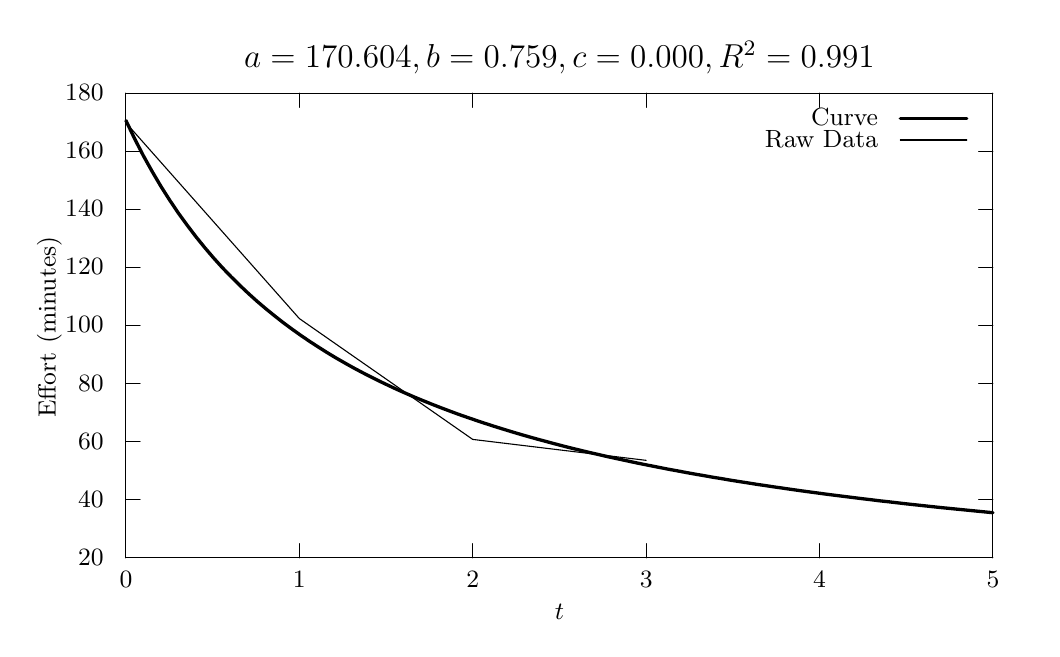
\begin{tikzpicture}[gnuplot]
%% generated with GNUPLOT 4.6p4 (Lua 5.1; terminal rev. 99, script rev. 100)
%% Fri 03 Oct 2014 12:39:55 WST
\tikzset{every node/.append style={font={\fontsize{9pt}{10.8pt}\selectfont}}}
\gpmonochromelines
\path (0.000,0.000) rectangle (12.700,7.620);
\gpcolor{color=gp lt color border}
\gpsetlinetype{gp lt border}
\gpsetlinewidth{1.00}
\draw[gp path] (1.190,0.886)--(1.370,0.886);
\draw[gp path] (12.201,0.886)--(12.021,0.886);
\node[gp node right] at (1.024,0.886) {20};
\draw[gp path] (1.190,1.624)--(1.370,1.624);
\draw[gp path] (12.201,1.624)--(12.021,1.624);
\node[gp node right] at (1.024,1.624) {40};
\draw[gp path] (1.190,2.362)--(1.370,2.362);
\draw[gp path] (12.201,2.362)--(12.021,2.362);
\node[gp node right] at (1.024,2.362) {60};
\draw[gp path] (1.190,3.099)--(1.370,3.099);
\draw[gp path] (12.201,3.099)--(12.021,3.099);
\node[gp node right] at (1.024,3.099) {80};
\draw[gp path] (1.190,3.837)--(1.370,3.837);
\draw[gp path] (12.201,3.837)--(12.021,3.837);
\node[gp node right] at (1.024,3.837) {100};
\draw[gp path] (1.190,4.575)--(1.370,4.575);
\draw[gp path] (12.201,4.575)--(12.021,4.575);
\node[gp node right] at (1.024,4.575) {120};
\draw[gp path] (1.190,5.313)--(1.370,5.313);
\draw[gp path] (12.201,5.313)--(12.021,5.313);
\node[gp node right] at (1.024,5.313) {140};
\draw[gp path] (1.190,6.050)--(1.370,6.050);
\draw[gp path] (12.201,6.050)--(12.021,6.050);
\node[gp node right] at (1.024,6.050) {160};
\draw[gp path] (1.190,6.788)--(1.370,6.788);
\draw[gp path] (12.201,6.788)--(12.021,6.788);
\node[gp node right] at (1.024,6.788) {180};
\draw[gp path] (1.190,0.886)--(1.190,1.066);
\draw[gp path] (1.190,6.788)--(1.190,6.608);
\node[gp node center] at (1.190,0.609) {0};
\draw[gp path] (3.392,0.886)--(3.392,1.066);
\draw[gp path] (3.392,6.788)--(3.392,6.608);
\node[gp node center] at (3.392,0.609) {1};
\draw[gp path] (5.594,0.886)--(5.594,1.066);
\draw[gp path] (5.594,6.788)--(5.594,6.608);
\node[gp node center] at (5.594,0.609) {2};
\draw[gp path] (7.797,0.886)--(7.797,1.066);
\draw[gp path] (7.797,6.788)--(7.797,6.608);
\node[gp node center] at (7.797,0.609) {3};
\draw[gp path] (9.999,0.886)--(9.999,1.066);
\draw[gp path] (9.999,6.788)--(9.999,6.608);
\node[gp node center] at (9.999,0.609) {4};
\draw[gp path] (12.201,0.886)--(12.201,1.066);
\draw[gp path] (12.201,6.788)--(12.201,6.608);
\node[gp node center] at (12.201,0.609) {5};
\draw[gp path] (1.190,6.788)--(1.190,0.886)--(12.201,0.886)--(12.201,6.788)--cycle;
\node[gp node center,rotate=-270] at (0.221,3.837) {Effort (minutes)};
\node[gp node center] at (6.695,0.194) {$t$};
\node[gp node center,font={\fontsize{12pt}{14.4pt}\selectfont}] at (6.695,7.204) {$a = 170.604, b = 0.759, c = 0.000, R^2 = 0.991$};
\node[gp node right] at (10.859,6.470) {Curve};
\gpcolor{color=gp lt color 0}
\gpsetlinetype{gp lt plot 0}
\gpsetlinewidth{3.00}
\draw[gp path] (11.025,6.470)--(11.869,6.470);
\draw[gp path] (1.190,6.441)--(1.301,6.209)--(1.412,5.993)--(1.524,5.792)--(1.635,5.604)%
  --(1.746,5.429)--(1.857,5.264)--(1.969,5.110)--(2.080,4.964)--(2.191,4.827)--(2.302,4.697)%
  --(2.413,4.574)--(2.525,4.458)--(2.636,4.348)--(2.747,4.243)--(2.858,4.143)--(2.970,4.048)%
  --(3.081,3.958)--(3.192,3.871)--(3.303,3.789)--(3.414,3.710)--(3.526,3.634)--(3.637,3.562)%
  --(3.748,3.492)--(3.859,3.425)--(3.971,3.361)--(4.082,3.299)--(4.193,3.240)--(4.304,3.183)%
  --(4.415,3.128)--(4.527,3.075)--(4.638,3.023)--(4.749,2.974)--(4.860,2.926)--(4.972,2.880)%
  --(5.083,2.835)--(5.194,2.792)--(5.305,2.750)--(5.416,2.709)--(5.528,2.670)--(5.639,2.632)%
  --(5.750,2.595)--(5.861,2.559)--(5.973,2.524)--(6.084,2.490)--(6.195,2.457)--(6.306,2.425)%
  --(6.417,2.394)--(6.529,2.364)--(6.640,2.334)--(6.751,2.305)--(6.862,2.277)--(6.974,2.250)%
  --(7.085,2.223)--(7.196,2.198)--(7.307,2.172)--(7.418,2.148)--(7.530,2.124)--(7.641,2.100)%
  --(7.752,2.077)--(7.863,2.055)--(7.975,2.033)--(8.086,2.011)--(8.197,1.991)--(8.308,1.970)%
  --(8.419,1.950)--(8.531,1.931)--(8.642,1.911)--(8.753,1.893)--(8.864,1.874)--(8.976,1.856)%
  --(9.087,1.839)--(9.198,1.821)--(9.309,1.805)--(9.420,1.788)--(9.532,1.772)--(9.643,1.756)%
  --(9.754,1.740)--(9.865,1.725)--(9.977,1.710)--(10.088,1.695)--(10.199,1.681)--(10.310,1.667)%
  --(10.421,1.653)--(10.533,1.639)--(10.644,1.626)--(10.755,1.612)--(10.866,1.600)--(10.978,1.587)%
  --(11.089,1.574)--(11.200,1.562)--(11.311,1.550)--(11.422,1.538)--(11.534,1.526)--(11.645,1.515)%
  --(11.756,1.504)--(11.867,1.493)--(11.979,1.482)--(12.090,1.471)--(12.201,1.460);
\gpcolor{color=gp lt color border}
\node[gp node right] at (10.859,6.193) {Raw Data};
\gpcolor{color=gp lt color 3}
\gpsetlinetype{gp lt plot 3}
\gpsetlinewidth{1.00}
\draw[gp path] (11.025,6.193)--(11.869,6.193);
\draw[gp path] (1.190,6.412)--(3.392,3.926)--(5.594,2.391)--(7.797,2.125);
\gpcolor{color=gp lt color border}
\gpsetlinetype{gp lt border}
\draw[gp path] (1.190,6.788)--(1.190,0.886)--(12.201,0.886)--(12.201,6.788)--cycle;
%% coordinates of the plot area
\gpdefrectangularnode{gp plot 1}{\pgfpoint{1.190cm}{0.886cm}}{\pgfpoint{12.201cm}{6.788cm}}
\end{tikzpicture}
%% gnuplot variables

  \caption{Problem 1 Language A}
  \end{figure}
  
  \begin{figure}[!htb]
  \centering
  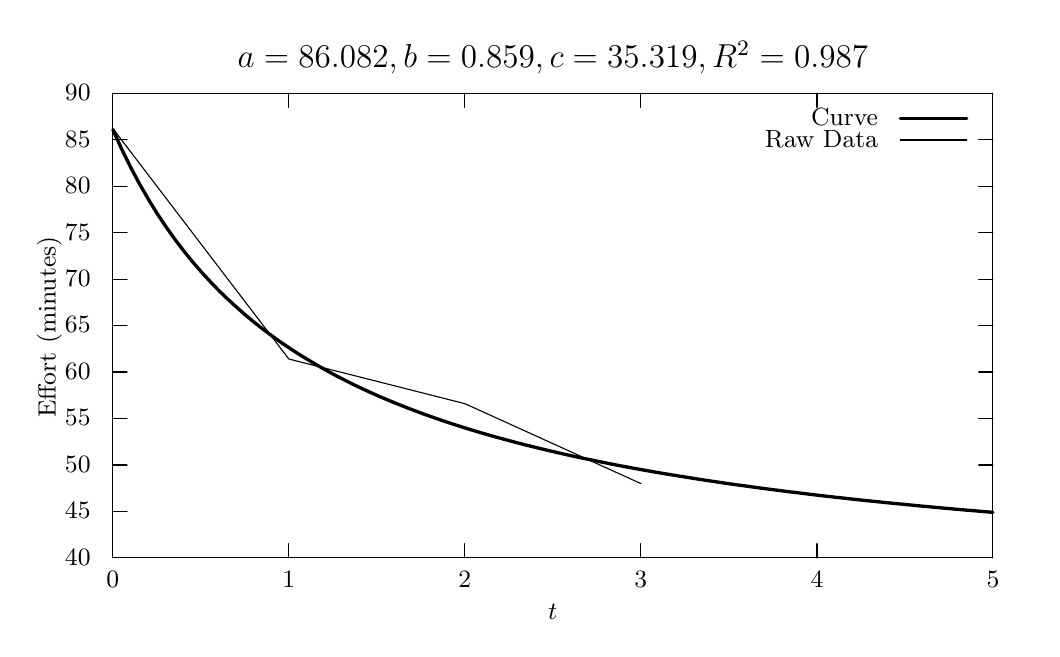
\begin{tikzpicture}[gnuplot]
%% generated with GNUPLOT 4.6p4 (Lua 5.1; terminal rev. 99, script rev. 100)
%% Fri 03 Oct 2014 12:39:55 WST
\tikzset{every node/.append style={font={\fontsize{9pt}{10.8pt}\selectfont}}}
\gpmonochromelines
\path (0.000,0.000) rectangle (12.700,7.620);
\gpcolor{color=gp lt color border}
\gpsetlinetype{gp lt border}
\gpsetlinewidth{1.00}
\draw[gp path] (1.024,0.886)--(1.204,0.886);
\draw[gp path] (12.201,0.886)--(12.021,0.886);
\node[gp node right] at (0.858,0.886) {40};
\draw[gp path] (1.024,1.476)--(1.204,1.476);
\draw[gp path] (12.201,1.476)--(12.021,1.476);
\node[gp node right] at (0.858,1.476) {45};
\draw[gp path] (1.024,2.066)--(1.204,2.066);
\draw[gp path] (12.201,2.066)--(12.021,2.066);
\node[gp node right] at (0.858,2.066) {50};
\draw[gp path] (1.024,2.657)--(1.204,2.657);
\draw[gp path] (12.201,2.657)--(12.021,2.657);
\node[gp node right] at (0.858,2.657) {55};
\draw[gp path] (1.024,3.247)--(1.204,3.247);
\draw[gp path] (12.201,3.247)--(12.021,3.247);
\node[gp node right] at (0.858,3.247) {60};
\draw[gp path] (1.024,3.837)--(1.204,3.837);
\draw[gp path] (12.201,3.837)--(12.021,3.837);
\node[gp node right] at (0.858,3.837) {65};
\draw[gp path] (1.024,4.427)--(1.204,4.427);
\draw[gp path] (12.201,4.427)--(12.021,4.427);
\node[gp node right] at (0.858,4.427) {70};
\draw[gp path] (1.024,5.017)--(1.204,5.017);
\draw[gp path] (12.201,5.017)--(12.021,5.017);
\node[gp node right] at (0.858,5.017) {75};
\draw[gp path] (1.024,5.608)--(1.204,5.608);
\draw[gp path] (12.201,5.608)--(12.021,5.608);
\node[gp node right] at (0.858,5.608) {80};
\draw[gp path] (1.024,6.198)--(1.204,6.198);
\draw[gp path] (12.201,6.198)--(12.021,6.198);
\node[gp node right] at (0.858,6.198) {85};
\draw[gp path] (1.024,6.788)--(1.204,6.788);
\draw[gp path] (12.201,6.788)--(12.021,6.788);
\node[gp node right] at (0.858,6.788) {90};
\draw[gp path] (1.024,0.886)--(1.024,1.066);
\draw[gp path] (1.024,6.788)--(1.024,6.608);
\node[gp node center] at (1.024,0.609) {0};
\draw[gp path] (3.259,0.886)--(3.259,1.066);
\draw[gp path] (3.259,6.788)--(3.259,6.608);
\node[gp node center] at (3.259,0.609) {1};
\draw[gp path] (5.495,0.886)--(5.495,1.066);
\draw[gp path] (5.495,6.788)--(5.495,6.608);
\node[gp node center] at (5.495,0.609) {2};
\draw[gp path] (7.730,0.886)--(7.730,1.066);
\draw[gp path] (7.730,6.788)--(7.730,6.608);
\node[gp node center] at (7.730,0.609) {3};
\draw[gp path] (9.966,0.886)--(9.966,1.066);
\draw[gp path] (9.966,6.788)--(9.966,6.608);
\node[gp node center] at (9.966,0.609) {4};
\draw[gp path] (12.201,0.886)--(12.201,1.066);
\draw[gp path] (12.201,6.788)--(12.201,6.608);
\node[gp node center] at (12.201,0.609) {5};
\draw[gp path] (1.024,6.788)--(1.024,0.886)--(12.201,0.886)--(12.201,6.788)--cycle;
\node[gp node center,rotate=-270] at (0.221,3.837) {Effort (minutes)};
\node[gp node center] at (6.612,0.194) {$t$};
\node[gp node center,font={\fontsize{12pt}{14.4pt}\selectfont}] at (6.612,7.204) {$a = 86.082, b = 0.859, c = 35.319, R^2 = 0.987$};
\node[gp node right] at (10.859,6.470) {Curve};
\gpcolor{color=gp lt color 0}
\gpsetlinetype{gp lt plot 0}
\gpsetlinewidth{3.00}
\draw[gp path] (11.025,6.470)--(11.869,6.470);
\draw[gp path] (1.024,6.326)--(1.137,6.076)--(1.250,5.847)--(1.363,5.635)--(1.476,5.439)%
  --(1.588,5.257)--(1.701,5.088)--(1.814,4.929)--(1.927,4.781)--(2.040,4.642)--(2.153,4.512)%
  --(2.266,4.389)--(2.379,4.273)--(2.492,4.164)--(2.605,4.061)--(2.717,3.963)--(2.830,3.870)%
  --(2.943,3.781)--(3.056,3.697)--(3.169,3.617)--(3.282,3.541)--(3.395,3.468)--(3.508,3.399)%
  --(3.621,3.332)--(3.734,3.268)--(3.846,3.207)--(3.959,3.149)--(4.072,3.092)--(4.185,3.038)%
  --(4.298,2.986)--(4.411,2.936)--(4.524,2.888)--(4.637,2.842)--(4.750,2.797)--(4.863,2.754)%
  --(4.975,2.712)--(5.088,2.672)--(5.201,2.633)--(5.314,2.595)--(5.427,2.559)--(5.540,2.523)%
  --(5.653,2.489)--(5.766,2.456)--(5.879,2.424)--(5.992,2.393)--(6.104,2.363)--(6.217,2.333)%
  --(6.330,2.305)--(6.443,2.277)--(6.556,2.250)--(6.669,2.224)--(6.782,2.198)--(6.895,2.173)%
  --(7.008,2.149)--(7.121,2.126)--(7.233,2.103)--(7.346,2.080)--(7.459,2.058)--(7.572,2.037)%
  --(7.685,2.016)--(7.798,1.996)--(7.911,1.976)--(8.024,1.957)--(8.137,1.938)--(8.250,1.920)%
  --(8.362,1.902)--(8.475,1.884)--(8.588,1.867)--(8.701,1.850)--(8.814,1.833)--(8.927,1.817)%
  --(9.040,1.802)--(9.153,1.786)--(9.266,1.771)--(9.379,1.756)--(9.491,1.742)--(9.604,1.727)%
  --(9.717,1.714)--(9.830,1.700)--(9.943,1.686)--(10.056,1.673)--(10.169,1.660)--(10.282,1.648)%
  --(10.395,1.635)--(10.508,1.623)--(10.620,1.611)--(10.733,1.600)--(10.846,1.588)--(10.959,1.577)%
  --(11.072,1.566)--(11.185,1.555)--(11.298,1.544)--(11.411,1.534)--(11.524,1.523)--(11.637,1.513)%
  --(11.749,1.503)--(11.862,1.493)--(11.975,1.484)--(12.088,1.474)--(12.201,1.465);
\gpcolor{color=gp lt color border}
\node[gp node right] at (10.859,6.193) {Raw Data};
\gpcolor{color=gp lt color 3}
\gpsetlinetype{gp lt plot 3}
\gpsetlinewidth{1.00}
\draw[gp path] (11.025,6.193)--(11.869,6.193);
\draw[gp path] (1.024,6.339)--(3.259,3.412)--(5.495,2.845)--(7.730,1.830);
\gpcolor{color=gp lt color border}
\gpsetlinetype{gp lt border}
\draw[gp path] (1.024,6.788)--(1.024,0.886)--(12.201,0.886)--(12.201,6.788)--cycle;
%% coordinates of the plot area
\gpdefrectangularnode{gp plot 1}{\pgfpoint{1.024cm}{0.886cm}}{\pgfpoint{12.201cm}{6.788cm}}
\end{tikzpicture}
%% gnuplot variables

  \caption{Problem 2 Language A}
  \end{figure}
  
  \begin{figure}[!htb]
  \centering
  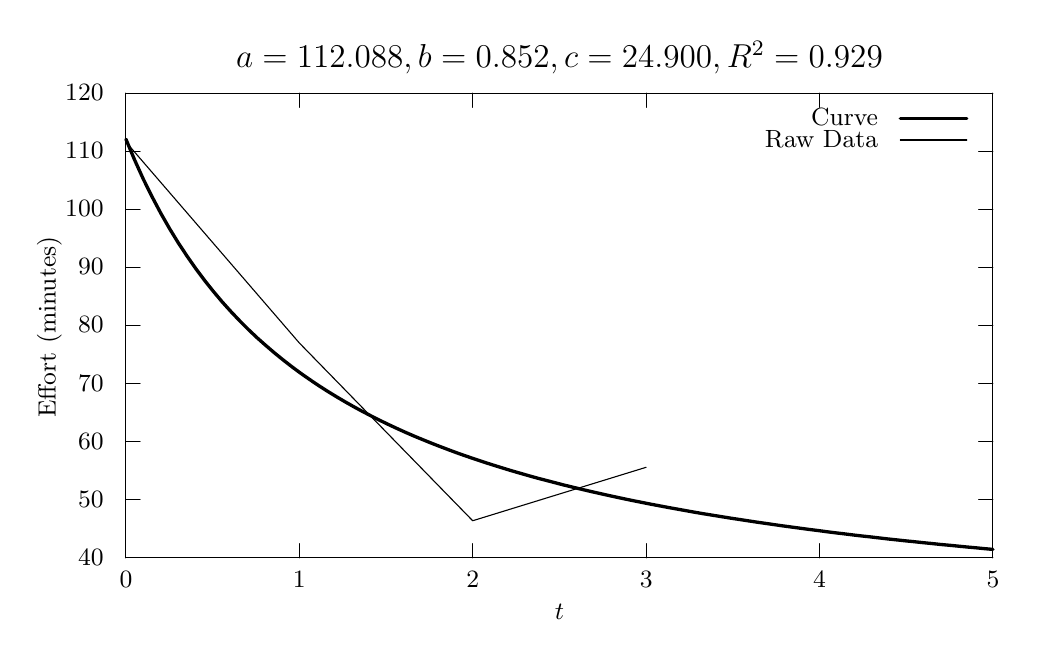
\begin{tikzpicture}[gnuplot]
%% generated with GNUPLOT 4.6p4 (Lua 5.1; terminal rev. 99, script rev. 100)
%% Fri 03 Oct 2014 12:39:55 WST
\tikzset{every node/.append style={font={\fontsize{9pt}{10.8pt}\selectfont}}}
\gpmonochromelines
\path (0.000,0.000) rectangle (12.700,7.620);
\gpcolor{color=gp lt color border}
\gpsetlinetype{gp lt border}
\gpsetlinewidth{1.00}
\draw[gp path] (1.190,0.886)--(1.370,0.886);
\draw[gp path] (12.201,0.886)--(12.021,0.886);
\node[gp node right] at (1.024,0.886) {40};
\draw[gp path] (1.190,1.624)--(1.370,1.624);
\draw[gp path] (12.201,1.624)--(12.021,1.624);
\node[gp node right] at (1.024,1.624) {50};
\draw[gp path] (1.190,2.362)--(1.370,2.362);
\draw[gp path] (12.201,2.362)--(12.021,2.362);
\node[gp node right] at (1.024,2.362) {60};
\draw[gp path] (1.190,3.099)--(1.370,3.099);
\draw[gp path] (12.201,3.099)--(12.021,3.099);
\node[gp node right] at (1.024,3.099) {70};
\draw[gp path] (1.190,3.837)--(1.370,3.837);
\draw[gp path] (12.201,3.837)--(12.021,3.837);
\node[gp node right] at (1.024,3.837) {80};
\draw[gp path] (1.190,4.575)--(1.370,4.575);
\draw[gp path] (12.201,4.575)--(12.021,4.575);
\node[gp node right] at (1.024,4.575) {90};
\draw[gp path] (1.190,5.313)--(1.370,5.313);
\draw[gp path] (12.201,5.313)--(12.021,5.313);
\node[gp node right] at (1.024,5.313) {100};
\draw[gp path] (1.190,6.050)--(1.370,6.050);
\draw[gp path] (12.201,6.050)--(12.021,6.050);
\node[gp node right] at (1.024,6.050) {110};
\draw[gp path] (1.190,6.788)--(1.370,6.788);
\draw[gp path] (12.201,6.788)--(12.021,6.788);
\node[gp node right] at (1.024,6.788) {120};
\draw[gp path] (1.190,0.886)--(1.190,1.066);
\draw[gp path] (1.190,6.788)--(1.190,6.608);
\node[gp node center] at (1.190,0.609) {0};
\draw[gp path] (3.392,0.886)--(3.392,1.066);
\draw[gp path] (3.392,6.788)--(3.392,6.608);
\node[gp node center] at (3.392,0.609) {1};
\draw[gp path] (5.594,0.886)--(5.594,1.066);
\draw[gp path] (5.594,6.788)--(5.594,6.608);
\node[gp node center] at (5.594,0.609) {2};
\draw[gp path] (7.797,0.886)--(7.797,1.066);
\draw[gp path] (7.797,6.788)--(7.797,6.608);
\node[gp node center] at (7.797,0.609) {3};
\draw[gp path] (9.999,0.886)--(9.999,1.066);
\draw[gp path] (9.999,6.788)--(9.999,6.608);
\node[gp node center] at (9.999,0.609) {4};
\draw[gp path] (12.201,0.886)--(12.201,1.066);
\draw[gp path] (12.201,6.788)--(12.201,6.608);
\node[gp node center] at (12.201,0.609) {5};
\draw[gp path] (1.190,6.788)--(1.190,0.886)--(12.201,0.886)--(12.201,6.788)--cycle;
\node[gp node center,rotate=-270] at (0.221,3.837) {Effort (minutes)};
\node[gp node center] at (6.695,0.194) {$t$};
\node[gp node center,font={\fontsize{12pt}{14.4pt}\selectfont}] at (6.695,7.204) {$a = 112.088, b = 0.852, c = 24.900, R^2 = 0.929$};
\node[gp node right] at (10.859,6.470) {Curve};
\gpcolor{color=gp lt color 0}
\gpsetlinetype{gp lt plot 0}
\gpsetlinewidth{3.00}
\draw[gp path] (11.025,6.470)--(11.869,6.470);
\draw[gp path] (1.190,6.204)--(1.301,5.939)--(1.412,5.694)--(1.524,5.469)--(1.635,5.259)%
  --(1.746,5.065)--(1.857,4.884)--(1.969,4.715)--(2.080,4.556)--(2.191,4.408)--(2.302,4.269)%
  --(2.413,4.137)--(2.525,4.013)--(2.636,3.896)--(2.747,3.785)--(2.858,3.680)--(2.970,3.581)%
  --(3.081,3.486)--(3.192,3.396)--(3.303,3.310)--(3.414,3.228)--(3.526,3.150)--(3.637,3.075)%
  --(3.748,3.004)--(3.859,2.936)--(3.971,2.870)--(4.082,2.807)--(4.193,2.747)--(4.304,2.689)%
  --(4.415,2.633)--(4.527,2.579)--(4.638,2.527)--(4.749,2.477)--(4.860,2.429)--(4.972,2.383)%
  --(5.083,2.338)--(5.194,2.295)--(5.305,2.253)--(5.416,2.212)--(5.528,2.173)--(5.639,2.135)%
  --(5.750,2.098)--(5.861,2.063)--(5.973,2.028)--(6.084,1.994)--(6.195,1.962)--(6.306,1.930)%
  --(6.417,1.899)--(6.529,1.870)--(6.640,1.841)--(6.751,1.812)--(6.862,1.785)--(6.974,1.758)%
  --(7.085,1.732)--(7.196,1.707)--(7.307,1.682)--(7.418,1.658)--(7.530,1.634)--(7.641,1.611)%
  --(7.752,1.589)--(7.863,1.567)--(7.975,1.546)--(8.086,1.525)--(8.197,1.505)--(8.308,1.485)%
  --(8.419,1.465)--(8.531,1.446)--(8.642,1.428)--(8.753,1.410)--(8.864,1.392)--(8.976,1.375)%
  --(9.087,1.358)--(9.198,1.341)--(9.309,1.325)--(9.420,1.309)--(9.532,1.293)--(9.643,1.278)%
  --(9.754,1.263)--(9.865,1.248)--(9.977,1.234)--(10.088,1.219)--(10.199,1.205)--(10.310,1.192)%
  --(10.421,1.178)--(10.533,1.165)--(10.644,1.153)--(10.755,1.140)--(10.866,1.127)--(10.978,1.115)%
  --(11.089,1.103)--(11.200,1.092)--(11.311,1.080)--(11.422,1.069)--(11.534,1.057)--(11.645,1.047)%
  --(11.756,1.036)--(11.867,1.025)--(11.979,1.015)--(12.090,1.004)--(12.201,0.994);
\gpcolor{color=gp lt color border}
\node[gp node right] at (10.859,6.193) {Raw Data};
\gpcolor{color=gp lt color 3}
\gpsetlinetype{gp lt plot 3}
\gpsetlinewidth{1.00}
\draw[gp path] (11.025,6.193)--(11.869,6.193);
\draw[gp path] (1.190,6.168)--(3.392,3.616)--(5.594,1.358)--(7.797,2.037);
\gpcolor{color=gp lt color border}
\gpsetlinetype{gp lt border}
\draw[gp path] (1.190,6.788)--(1.190,0.886)--(12.201,0.886)--(12.201,6.788)--cycle;
%% coordinates of the plot area
\gpdefrectangularnode{gp plot 1}{\pgfpoint{1.190cm}{0.886cm}}{\pgfpoint{12.201cm}{6.788cm}}
\end{tikzpicture}
%% gnuplot variables

  \caption{Problem 1 Language B}
  \end{figure}
  
  \FloatBarrier
  \subsection{Model B}
  $$(a-c)(t+1)^{-b}+c$$
  
  \begin{figure}[!htb]
  \centering
  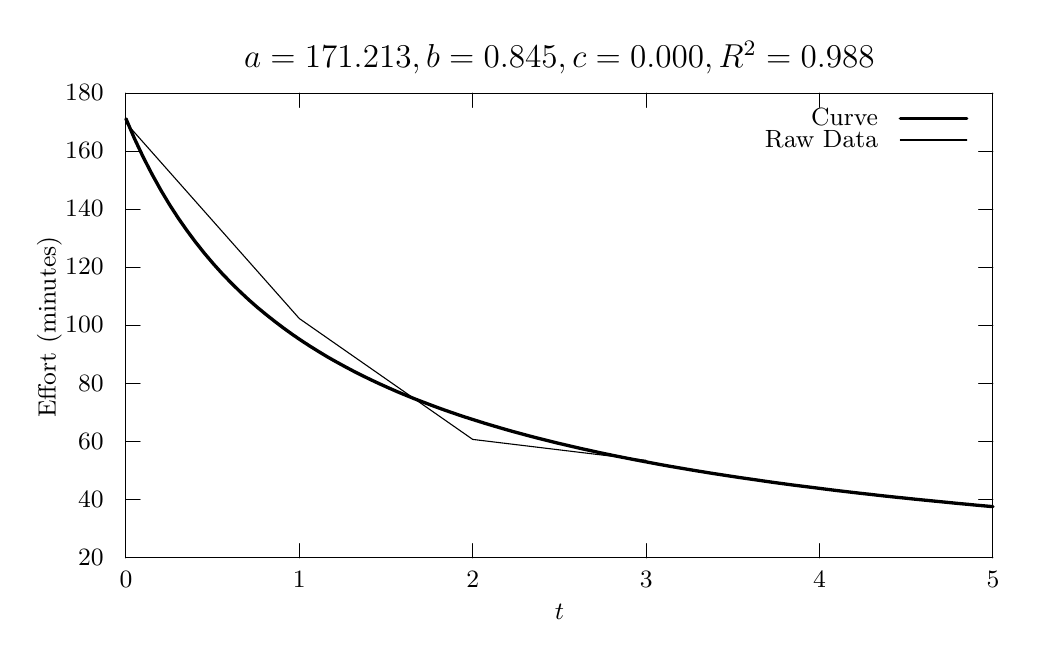
\begin{tikzpicture}[gnuplot]
%% generated with GNUPLOT 4.6p4 (Lua 5.1; terminal rev. 99, script rev. 100)
%% Fri 03 Oct 2014 12:39:55 WST
\tikzset{every node/.append style={font={\fontsize{9pt}{10.8pt}\selectfont}}}
\gpmonochromelines
\path (0.000,0.000) rectangle (12.700,7.620);
\gpcolor{color=gp lt color border}
\gpsetlinetype{gp lt border}
\gpsetlinewidth{1.00}
\draw[gp path] (1.190,0.886)--(1.370,0.886);
\draw[gp path] (12.201,0.886)--(12.021,0.886);
\node[gp node right] at (1.024,0.886) {20};
\draw[gp path] (1.190,1.624)--(1.370,1.624);
\draw[gp path] (12.201,1.624)--(12.021,1.624);
\node[gp node right] at (1.024,1.624) {40};
\draw[gp path] (1.190,2.362)--(1.370,2.362);
\draw[gp path] (12.201,2.362)--(12.021,2.362);
\node[gp node right] at (1.024,2.362) {60};
\draw[gp path] (1.190,3.099)--(1.370,3.099);
\draw[gp path] (12.201,3.099)--(12.021,3.099);
\node[gp node right] at (1.024,3.099) {80};
\draw[gp path] (1.190,3.837)--(1.370,3.837);
\draw[gp path] (12.201,3.837)--(12.021,3.837);
\node[gp node right] at (1.024,3.837) {100};
\draw[gp path] (1.190,4.575)--(1.370,4.575);
\draw[gp path] (12.201,4.575)--(12.021,4.575);
\node[gp node right] at (1.024,4.575) {120};
\draw[gp path] (1.190,5.313)--(1.370,5.313);
\draw[gp path] (12.201,5.313)--(12.021,5.313);
\node[gp node right] at (1.024,5.313) {140};
\draw[gp path] (1.190,6.050)--(1.370,6.050);
\draw[gp path] (12.201,6.050)--(12.021,6.050);
\node[gp node right] at (1.024,6.050) {160};
\draw[gp path] (1.190,6.788)--(1.370,6.788);
\draw[gp path] (12.201,6.788)--(12.021,6.788);
\node[gp node right] at (1.024,6.788) {180};
\draw[gp path] (1.190,0.886)--(1.190,1.066);
\draw[gp path] (1.190,6.788)--(1.190,6.608);
\node[gp node center] at (1.190,0.609) {0};
\draw[gp path] (3.392,0.886)--(3.392,1.066);
\draw[gp path] (3.392,6.788)--(3.392,6.608);
\node[gp node center] at (3.392,0.609) {1};
\draw[gp path] (5.594,0.886)--(5.594,1.066);
\draw[gp path] (5.594,6.788)--(5.594,6.608);
\node[gp node center] at (5.594,0.609) {2};
\draw[gp path] (7.797,0.886)--(7.797,1.066);
\draw[gp path] (7.797,6.788)--(7.797,6.608);
\node[gp node center] at (7.797,0.609) {3};
\draw[gp path] (9.999,0.886)--(9.999,1.066);
\draw[gp path] (9.999,6.788)--(9.999,6.608);
\node[gp node center] at (9.999,0.609) {4};
\draw[gp path] (12.201,0.886)--(12.201,1.066);
\draw[gp path] (12.201,6.788)--(12.201,6.608);
\node[gp node center] at (12.201,0.609) {5};
\draw[gp path] (1.190,6.788)--(1.190,0.886)--(12.201,0.886)--(12.201,6.788)--cycle;
\node[gp node center,rotate=-270] at (0.221,3.837) {Effort (minutes)};
\node[gp node center] at (6.695,0.194) {$t$};
\node[gp node center,font={\fontsize{12pt}{14.4pt}\selectfont}] at (6.695,7.204) {$a = 171.213, b = 0.845, c = 0.000, R^2 = 0.988$};
\node[gp node right] at (10.859,6.470) {Curve};
\gpcolor{color=gp lt color 0}
\gpsetlinetype{gp lt plot 0}
\gpsetlinewidth{3.00}
\draw[gp path] (11.025,6.470)--(11.869,6.470);
\draw[gp path] (1.190,6.464)--(1.301,6.206)--(1.412,5.971)--(1.524,5.754)--(1.635,5.554)%
  --(1.746,5.369)--(1.857,5.198)--(1.969,5.038)--(2.080,4.889)--(2.191,4.750)--(2.302,4.619)%
  --(2.413,4.496)--(2.525,4.380)--(2.636,4.271)--(2.747,4.167)--(2.858,4.069)--(2.970,3.977)%
  --(3.081,3.889)--(3.192,3.805)--(3.303,3.725)--(3.414,3.649)--(3.526,3.576)--(3.637,3.507)%
  --(3.748,3.440)--(3.859,3.377)--(3.971,3.316)--(4.082,3.257)--(4.193,3.201)--(4.304,3.147)%
  --(4.415,3.095)--(4.527,3.045)--(4.638,2.996)--(4.749,2.950)--(4.860,2.905)--(4.972,2.862)%
  --(5.083,2.820)--(5.194,2.779)--(5.305,2.740)--(5.416,2.702)--(5.528,2.665)--(5.639,2.630)%
  --(5.750,2.595)--(5.861,2.562)--(5.973,2.529)--(6.084,2.497)--(6.195,2.467)--(6.306,2.437)%
  --(6.417,2.408)--(6.529,2.380)--(6.640,2.352)--(6.751,2.326)--(6.862,2.300)--(6.974,2.274)%
  --(7.085,2.250)--(7.196,2.225)--(7.307,2.202)--(7.418,2.179)--(7.530,2.157)--(7.641,2.135)%
  --(7.752,2.114)--(7.863,2.093)--(7.975,2.072)--(8.086,2.052)--(8.197,2.033)--(8.308,2.014)%
  --(8.419,1.995)--(8.531,1.977)--(8.642,1.959)--(8.753,1.942)--(8.864,1.925)--(8.976,1.908)%
  --(9.087,1.892)--(9.198,1.876)--(9.309,1.860)--(9.420,1.844)--(9.532,1.829)--(9.643,1.814)%
  --(9.754,1.800)--(9.865,1.786)--(9.977,1.772)--(10.088,1.758)--(10.199,1.744)--(10.310,1.731)%
  --(10.421,1.718)--(10.533,1.705)--(10.644,1.693)--(10.755,1.680)--(10.866,1.668)--(10.978,1.656)%
  --(11.089,1.645)--(11.200,1.633)--(11.311,1.622)--(11.422,1.611)--(11.534,1.600)--(11.645,1.589)%
  --(11.756,1.578)--(11.867,1.568)--(11.979,1.557)--(12.090,1.547)--(12.201,1.537);
\gpcolor{color=gp lt color border}
\node[gp node right] at (10.859,6.193) {Raw Data};
\gpcolor{color=gp lt color 3}
\gpsetlinetype{gp lt plot 3}
\gpsetlinewidth{1.00}
\draw[gp path] (11.025,6.193)--(11.869,6.193);
\draw[gp path] (1.190,6.412)--(3.392,3.926)--(5.594,2.391)--(7.797,2.125);
\gpcolor{color=gp lt color border}
\gpsetlinetype{gp lt border}
\draw[gp path] (1.190,6.788)--(1.190,0.886)--(12.201,0.886)--(12.201,6.788)--cycle;
%% coordinates of the plot area
\gpdefrectangularnode{gp plot 1}{\pgfpoint{1.190cm}{0.886cm}}{\pgfpoint{12.201cm}{6.788cm}}
\end{tikzpicture}
%% gnuplot variables

  \caption{Problem 1 Language A}
  \end{figure}
  
  \begin{figure}[!htb]
  \centering
  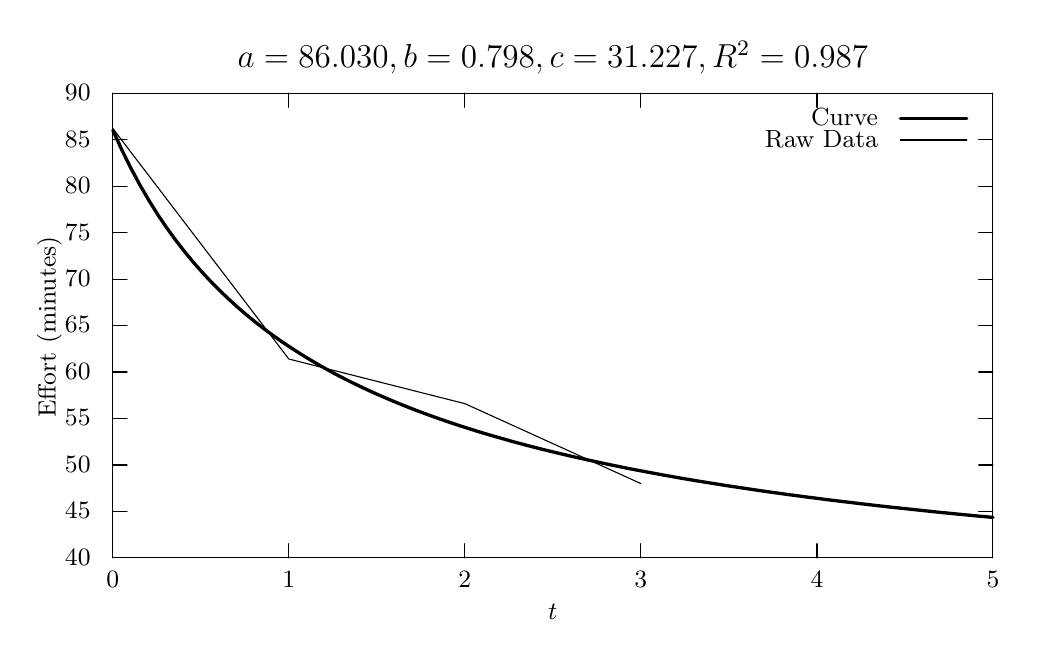
\begin{tikzpicture}[gnuplot]
%% generated with GNUPLOT 4.6p4 (Lua 5.1; terminal rev. 99, script rev. 100)
%% Fri 03 Oct 2014 12:39:55 WST
\tikzset{every node/.append style={font={\fontsize{9pt}{10.8pt}\selectfont}}}
\gpmonochromelines
\path (0.000,0.000) rectangle (12.700,7.620);
\gpcolor{color=gp lt color border}
\gpsetlinetype{gp lt border}
\gpsetlinewidth{1.00}
\draw[gp path] (1.024,0.886)--(1.204,0.886);
\draw[gp path] (12.201,0.886)--(12.021,0.886);
\node[gp node right] at (0.858,0.886) {40};
\draw[gp path] (1.024,1.476)--(1.204,1.476);
\draw[gp path] (12.201,1.476)--(12.021,1.476);
\node[gp node right] at (0.858,1.476) {45};
\draw[gp path] (1.024,2.066)--(1.204,2.066);
\draw[gp path] (12.201,2.066)--(12.021,2.066);
\node[gp node right] at (0.858,2.066) {50};
\draw[gp path] (1.024,2.657)--(1.204,2.657);
\draw[gp path] (12.201,2.657)--(12.021,2.657);
\node[gp node right] at (0.858,2.657) {55};
\draw[gp path] (1.024,3.247)--(1.204,3.247);
\draw[gp path] (12.201,3.247)--(12.021,3.247);
\node[gp node right] at (0.858,3.247) {60};
\draw[gp path] (1.024,3.837)--(1.204,3.837);
\draw[gp path] (12.201,3.837)--(12.021,3.837);
\node[gp node right] at (0.858,3.837) {65};
\draw[gp path] (1.024,4.427)--(1.204,4.427);
\draw[gp path] (12.201,4.427)--(12.021,4.427);
\node[gp node right] at (0.858,4.427) {70};
\draw[gp path] (1.024,5.017)--(1.204,5.017);
\draw[gp path] (12.201,5.017)--(12.021,5.017);
\node[gp node right] at (0.858,5.017) {75};
\draw[gp path] (1.024,5.608)--(1.204,5.608);
\draw[gp path] (12.201,5.608)--(12.021,5.608);
\node[gp node right] at (0.858,5.608) {80};
\draw[gp path] (1.024,6.198)--(1.204,6.198);
\draw[gp path] (12.201,6.198)--(12.021,6.198);
\node[gp node right] at (0.858,6.198) {85};
\draw[gp path] (1.024,6.788)--(1.204,6.788);
\draw[gp path] (12.201,6.788)--(12.021,6.788);
\node[gp node right] at (0.858,6.788) {90};
\draw[gp path] (1.024,0.886)--(1.024,1.066);
\draw[gp path] (1.024,6.788)--(1.024,6.608);
\node[gp node center] at (1.024,0.609) {0};
\draw[gp path] (3.259,0.886)--(3.259,1.066);
\draw[gp path] (3.259,6.788)--(3.259,6.608);
\node[gp node center] at (3.259,0.609) {1};
\draw[gp path] (5.495,0.886)--(5.495,1.066);
\draw[gp path] (5.495,6.788)--(5.495,6.608);
\node[gp node center] at (5.495,0.609) {2};
\draw[gp path] (7.730,0.886)--(7.730,1.066);
\draw[gp path] (7.730,6.788)--(7.730,6.608);
\node[gp node center] at (7.730,0.609) {3};
\draw[gp path] (9.966,0.886)--(9.966,1.066);
\draw[gp path] (9.966,6.788)--(9.966,6.608);
\node[gp node center] at (9.966,0.609) {4};
\draw[gp path] (12.201,0.886)--(12.201,1.066);
\draw[gp path] (12.201,6.788)--(12.201,6.608);
\node[gp node center] at (12.201,0.609) {5};
\draw[gp path] (1.024,6.788)--(1.024,0.886)--(12.201,0.886)--(12.201,6.788)--cycle;
\node[gp node center,rotate=-270] at (0.221,3.837) {Effort (minutes)};
\node[gp node center] at (6.612,0.194) {$t$};
\node[gp node center,font={\fontsize{12pt}{14.4pt}\selectfont}] at (6.612,7.204) {$a = 86.030, b = 0.798, c = 31.227, R^2 = 0.987$};
\node[gp node right] at (10.859,6.470) {Curve};
\gpcolor{color=gp lt color 0}
\gpsetlinetype{gp lt plot 0}
\gpsetlinewidth{3.00}
\draw[gp path] (11.025,6.470)--(11.869,6.470);
\draw[gp path] (1.024,6.319)--(1.137,6.070)--(1.250,5.842)--(1.363,5.631)--(1.476,5.436)%
  --(1.588,5.256)--(1.701,5.088)--(1.814,4.932)--(1.927,4.786)--(2.040,4.648)--(2.153,4.520)%
  --(2.266,4.398)--(2.379,4.284)--(2.492,4.176)--(2.605,4.073)--(2.717,3.976)--(2.830,3.884)%
  --(2.943,3.796)--(3.056,3.713)--(3.169,3.633)--(3.282,3.557)--(3.395,3.485)--(3.508,3.415)%
  --(3.621,3.349)--(3.734,3.285)--(3.846,3.223)--(3.959,3.165)--(4.072,3.108)--(4.185,3.054)%
  --(4.298,3.001)--(4.411,2.951)--(4.524,2.902)--(4.637,2.855)--(4.750,2.809)--(4.863,2.765)%
  --(4.975,2.723)--(5.088,2.682)--(5.201,2.642)--(5.314,2.603)--(5.427,2.566)--(5.540,2.530)%
  --(5.653,2.494)--(5.766,2.460)--(5.879,2.427)--(5.992,2.395)--(6.104,2.363)--(6.217,2.333)%
  --(6.330,2.303)--(6.443,2.274)--(6.556,2.246)--(6.669,2.219)--(6.782,2.192)--(6.895,2.166)%
  --(7.008,2.141)--(7.121,2.116)--(7.233,2.092)--(7.346,2.068)--(7.459,2.045)--(7.572,2.022)%
  --(7.685,2.000)--(7.798,1.979)--(7.911,1.958)--(8.024,1.937)--(8.137,1.917)--(8.250,1.897)%
  --(8.362,1.878)--(8.475,1.859)--(8.588,1.841)--(8.701,1.823)--(8.814,1.805)--(8.927,1.788)%
  --(9.040,1.771)--(9.153,1.754)--(9.266,1.737)--(9.379,1.721)--(9.491,1.706)--(9.604,1.690)%
  --(9.717,1.675)--(9.830,1.660)--(9.943,1.646)--(10.056,1.631)--(10.169,1.617)--(10.282,1.603)%
  --(10.395,1.590)--(10.508,1.576)--(10.620,1.563)--(10.733,1.550)--(10.846,1.537)--(10.959,1.525)%
  --(11.072,1.513)--(11.185,1.501)--(11.298,1.489)--(11.411,1.477)--(11.524,1.465)--(11.637,1.454)%
  --(11.749,1.443)--(11.862,1.432)--(11.975,1.421)--(12.088,1.411)--(12.201,1.400);
\gpcolor{color=gp lt color border}
\node[gp node right] at (10.859,6.193) {Raw Data};
\gpcolor{color=gp lt color 3}
\gpsetlinetype{gp lt plot 3}
\gpsetlinewidth{1.00}
\draw[gp path] (11.025,6.193)--(11.869,6.193);
\draw[gp path] (1.024,6.339)--(3.259,3.412)--(5.495,2.845)--(7.730,1.830);
\gpcolor{color=gp lt color border}
\gpsetlinetype{gp lt border}
\draw[gp path] (1.024,6.788)--(1.024,0.886)--(12.201,0.886)--(12.201,6.788)--cycle;
%% coordinates of the plot area
\gpdefrectangularnode{gp plot 1}{\pgfpoint{1.024cm}{0.886cm}}{\pgfpoint{12.201cm}{6.788cm}}
\end{tikzpicture}
%% gnuplot variables

  \caption{Problem 2 Language A}
  \end{figure}
  
  \begin{figure}[!htb]
  \centering
  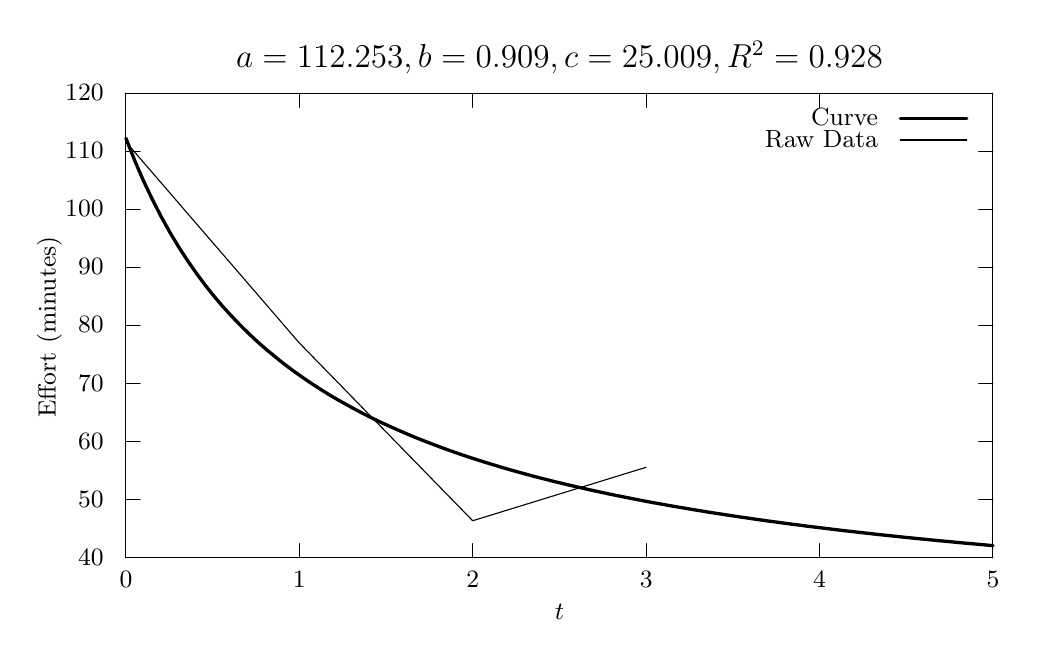
\begin{tikzpicture}[gnuplot]
%% generated with GNUPLOT 4.6p4 (Lua 5.1; terminal rev. 99, script rev. 100)
%% Fri 03 Oct 2014 12:39:55 WST
\tikzset{every node/.append style={font={\fontsize{9pt}{10.8pt}\selectfont}}}
\gpmonochromelines
\path (0.000,0.000) rectangle (12.700,7.620);
\gpcolor{color=gp lt color border}
\gpsetlinetype{gp lt border}
\gpsetlinewidth{1.00}
\draw[gp path] (1.190,0.886)--(1.370,0.886);
\draw[gp path] (12.201,0.886)--(12.021,0.886);
\node[gp node right] at (1.024,0.886) {40};
\draw[gp path] (1.190,1.624)--(1.370,1.624);
\draw[gp path] (12.201,1.624)--(12.021,1.624);
\node[gp node right] at (1.024,1.624) {50};
\draw[gp path] (1.190,2.362)--(1.370,2.362);
\draw[gp path] (12.201,2.362)--(12.021,2.362);
\node[gp node right] at (1.024,2.362) {60};
\draw[gp path] (1.190,3.099)--(1.370,3.099);
\draw[gp path] (12.201,3.099)--(12.021,3.099);
\node[gp node right] at (1.024,3.099) {70};
\draw[gp path] (1.190,3.837)--(1.370,3.837);
\draw[gp path] (12.201,3.837)--(12.021,3.837);
\node[gp node right] at (1.024,3.837) {80};
\draw[gp path] (1.190,4.575)--(1.370,4.575);
\draw[gp path] (12.201,4.575)--(12.021,4.575);
\node[gp node right] at (1.024,4.575) {90};
\draw[gp path] (1.190,5.313)--(1.370,5.313);
\draw[gp path] (12.201,5.313)--(12.021,5.313);
\node[gp node right] at (1.024,5.313) {100};
\draw[gp path] (1.190,6.050)--(1.370,6.050);
\draw[gp path] (12.201,6.050)--(12.021,6.050);
\node[gp node right] at (1.024,6.050) {110};
\draw[gp path] (1.190,6.788)--(1.370,6.788);
\draw[gp path] (12.201,6.788)--(12.021,6.788);
\node[gp node right] at (1.024,6.788) {120};
\draw[gp path] (1.190,0.886)--(1.190,1.066);
\draw[gp path] (1.190,6.788)--(1.190,6.608);
\node[gp node center] at (1.190,0.609) {0};
\draw[gp path] (3.392,0.886)--(3.392,1.066);
\draw[gp path] (3.392,6.788)--(3.392,6.608);
\node[gp node center] at (3.392,0.609) {1};
\draw[gp path] (5.594,0.886)--(5.594,1.066);
\draw[gp path] (5.594,6.788)--(5.594,6.608);
\node[gp node center] at (5.594,0.609) {2};
\draw[gp path] (7.797,0.886)--(7.797,1.066);
\draw[gp path] (7.797,6.788)--(7.797,6.608);
\node[gp node center] at (7.797,0.609) {3};
\draw[gp path] (9.999,0.886)--(9.999,1.066);
\draw[gp path] (9.999,6.788)--(9.999,6.608);
\node[gp node center] at (9.999,0.609) {4};
\draw[gp path] (12.201,0.886)--(12.201,1.066);
\draw[gp path] (12.201,6.788)--(12.201,6.608);
\node[gp node center] at (12.201,0.609) {5};
\draw[gp path] (1.190,6.788)--(1.190,0.886)--(12.201,0.886)--(12.201,6.788)--cycle;
\node[gp node center,rotate=-270] at (0.221,3.837) {Effort (minutes)};
\node[gp node center] at (6.695,0.194) {$t$};
\node[gp node center,font={\fontsize{12pt}{14.4pt}\selectfont}] at (6.695,7.204) {$a = 112.253, b = 0.909, c = 25.009, R^2 = 0.928$};
\node[gp node right] at (10.859,6.470) {Curve};
\gpcolor{color=gp lt color 0}
\gpsetlinetype{gp lt plot 0}
\gpsetlinewidth{3.00}
\draw[gp path] (11.025,6.470)--(11.869,6.470);
\draw[gp path] (1.190,6.216)--(1.301,5.934)--(1.412,5.677)--(1.524,5.442)--(1.635,5.225)%
  --(1.746,5.025)--(1.857,4.840)--(1.969,4.668)--(2.080,4.508)--(2.191,4.358)--(2.302,4.218)%
  --(2.413,4.087)--(2.525,3.964)--(2.636,3.848)--(2.747,3.738)--(2.858,3.634)--(2.970,3.536)%
  --(3.081,3.444)--(3.192,3.355)--(3.303,3.271)--(3.414,3.192)--(3.526,3.115)--(3.637,3.043)%
  --(3.748,2.973)--(3.859,2.907)--(3.971,2.844)--(4.082,2.783)--(4.193,2.724)--(4.304,2.668)%
  --(4.415,2.614)--(4.527,2.563)--(4.638,2.513)--(4.749,2.465)--(4.860,2.418)--(4.972,2.374)%
  --(5.083,2.331)--(5.194,2.289)--(5.305,2.249)--(5.416,2.210)--(5.528,2.172)--(5.639,2.136)%
  --(5.750,2.101)--(5.861,2.067)--(5.973,2.033)--(6.084,2.001)--(6.195,1.970)--(6.306,1.940)%
  --(6.417,1.910)--(6.529,1.882)--(6.640,1.854)--(6.751,1.827)--(6.862,1.801)--(6.974,1.775)%
  --(7.085,1.750)--(7.196,1.726)--(7.307,1.702)--(7.418,1.679)--(7.530,1.657)--(7.641,1.635)%
  --(7.752,1.613)--(7.863,1.592)--(7.975,1.572)--(8.086,1.552)--(8.197,1.533)--(8.308,1.514)%
  --(8.419,1.495)--(8.531,1.477)--(8.642,1.459)--(8.753,1.442)--(8.864,1.425)--(8.976,1.408)%
  --(9.087,1.392)--(9.198,1.376)--(9.309,1.360)--(9.420,1.345)--(9.532,1.330)--(9.643,1.315)%
  --(9.754,1.301)--(9.865,1.286)--(9.977,1.273)--(10.088,1.259)--(10.199,1.246)--(10.310,1.232)%
  --(10.421,1.220)--(10.533,1.207)--(10.644,1.195)--(10.755,1.182)--(10.866,1.171)--(10.978,1.159)%
  --(11.089,1.147)--(11.200,1.136)--(11.311,1.125)--(11.422,1.114)--(11.534,1.103)--(11.645,1.093)%
  --(11.756,1.082)--(11.867,1.072)--(11.979,1.062)--(12.090,1.052)--(12.201,1.042);
\gpcolor{color=gp lt color border}
\node[gp node right] at (10.859,6.193) {Raw Data};
\gpcolor{color=gp lt color 3}
\gpsetlinetype{gp lt plot 3}
\gpsetlinewidth{1.00}
\draw[gp path] (11.025,6.193)--(11.869,6.193);
\draw[gp path] (1.190,6.168)--(3.392,3.616)--(5.594,1.358)--(7.797,2.037);
\gpcolor{color=gp lt color border}
\gpsetlinetype{gp lt border}
\draw[gp path] (1.190,6.788)--(1.190,0.886)--(12.201,0.886)--(12.201,6.788)--cycle;
%% coordinates of the plot area
\gpdefrectangularnode{gp plot 1}{\pgfpoint{1.190cm}{0.886cm}}{\pgfpoint{12.201cm}{6.788cm}}
\end{tikzpicture}
%% gnuplot variables

  \caption{Problem 1 Language B}
  \end{figure}
  
  \FloatBarrier
  \clearpage
  \subsection{Model C}
  $$(a-c) e^{-bt} + c$$
  
  \begin{figure}[!htb]
  \centering
  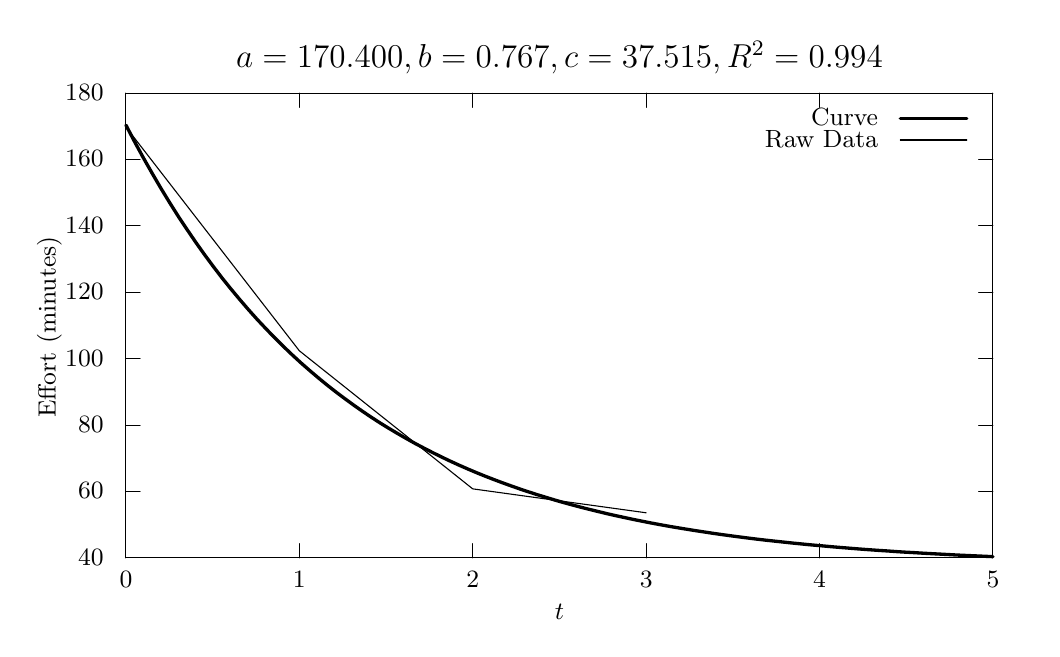
\begin{tikzpicture}[gnuplot]
%% generated with GNUPLOT 4.6p4 (Lua 5.1; terminal rev. 99, script rev. 100)
%% Fri 03 Oct 2014 12:39:55 WST
\tikzset{every node/.append style={font={\fontsize{9pt}{10.8pt}\selectfont}}}
\gpmonochromelines
\path (0.000,0.000) rectangle (12.700,7.620);
\gpcolor{color=gp lt color border}
\gpsetlinetype{gp lt border}
\gpsetlinewidth{1.00}
\draw[gp path] (1.190,0.886)--(1.370,0.886);
\draw[gp path] (12.201,0.886)--(12.021,0.886);
\node[gp node right] at (1.024,0.886) {40};
\draw[gp path] (1.190,1.729)--(1.370,1.729);
\draw[gp path] (12.201,1.729)--(12.021,1.729);
\node[gp node right] at (1.024,1.729) {60};
\draw[gp path] (1.190,2.572)--(1.370,2.572);
\draw[gp path] (12.201,2.572)--(12.021,2.572);
\node[gp node right] at (1.024,2.572) {80};
\draw[gp path] (1.190,3.415)--(1.370,3.415);
\draw[gp path] (12.201,3.415)--(12.021,3.415);
\node[gp node right] at (1.024,3.415) {100};
\draw[gp path] (1.190,4.259)--(1.370,4.259);
\draw[gp path] (12.201,4.259)--(12.021,4.259);
\node[gp node right] at (1.024,4.259) {120};
\draw[gp path] (1.190,5.102)--(1.370,5.102);
\draw[gp path] (12.201,5.102)--(12.021,5.102);
\node[gp node right] at (1.024,5.102) {140};
\draw[gp path] (1.190,5.945)--(1.370,5.945);
\draw[gp path] (12.201,5.945)--(12.021,5.945);
\node[gp node right] at (1.024,5.945) {160};
\draw[gp path] (1.190,6.788)--(1.370,6.788);
\draw[gp path] (12.201,6.788)--(12.021,6.788);
\node[gp node right] at (1.024,6.788) {180};
\draw[gp path] (1.190,0.886)--(1.190,1.066);
\draw[gp path] (1.190,6.788)--(1.190,6.608);
\node[gp node center] at (1.190,0.609) {0};
\draw[gp path] (3.392,0.886)--(3.392,1.066);
\draw[gp path] (3.392,6.788)--(3.392,6.608);
\node[gp node center] at (3.392,0.609) {1};
\draw[gp path] (5.594,0.886)--(5.594,1.066);
\draw[gp path] (5.594,6.788)--(5.594,6.608);
\node[gp node center] at (5.594,0.609) {2};
\draw[gp path] (7.797,0.886)--(7.797,1.066);
\draw[gp path] (7.797,6.788)--(7.797,6.608);
\node[gp node center] at (7.797,0.609) {3};
\draw[gp path] (9.999,0.886)--(9.999,1.066);
\draw[gp path] (9.999,6.788)--(9.999,6.608);
\node[gp node center] at (9.999,0.609) {4};
\draw[gp path] (12.201,0.886)--(12.201,1.066);
\draw[gp path] (12.201,6.788)--(12.201,6.608);
\node[gp node center] at (12.201,0.609) {5};
\draw[gp path] (1.190,6.788)--(1.190,0.886)--(12.201,0.886)--(12.201,6.788)--cycle;
\node[gp node center,rotate=-270] at (0.221,3.837) {Effort (minutes)};
\node[gp node center] at (6.695,0.194) {$t$};
\node[gp node center,font={\fontsize{12pt}{14.4pt}\selectfont}] at (6.695,7.204) {$a = 170.400, b = 0.767, c = 37.515, R^2 = 0.994$};
\node[gp node right] at (10.859,6.470) {Curve};
\gpcolor{color=gp lt color 0}
\gpsetlinetype{gp lt plot 0}
\gpsetlinewidth{3.00}
\draw[gp path] (11.025,6.470)--(11.869,6.470);
\draw[gp path] (1.190,6.383)--(1.301,6.170)--(1.412,5.966)--(1.524,5.769)--(1.635,5.579)%
  --(1.746,5.397)--(1.857,5.221)--(1.969,5.053)--(2.080,4.890)--(2.191,4.734)--(2.302,4.584)%
  --(2.413,4.439)--(2.525,4.300)--(2.636,4.167)--(2.747,4.038)--(2.858,3.914)--(2.970,3.795)%
  --(3.081,3.680)--(3.192,3.570)--(3.303,3.464)--(3.414,3.362)--(3.526,3.264)--(3.637,3.170)%
  --(3.748,3.079)--(3.859,2.992)--(3.971,2.908)--(4.082,2.827)--(4.193,2.749)--(4.304,2.674)%
  --(4.415,2.602)--(4.527,2.533)--(4.638,2.467)--(4.749,2.403)--(4.860,2.341)--(4.972,2.282)%
  --(5.083,2.225)--(5.194,2.170)--(5.305,2.117)--(5.416,2.066)--(5.528,2.017)--(5.639,1.970)%
  --(5.750,1.925)--(5.861,1.882)--(5.973,1.840)--(6.084,1.800)--(6.195,1.761)--(6.306,1.724)%
  --(6.417,1.688)--(6.529,1.654)--(6.640,1.620)--(6.751,1.588)--(6.862,1.558)--(6.974,1.528)%
  --(7.085,1.500)--(7.196,1.473)--(7.307,1.446)--(7.418,1.421)--(7.530,1.397)--(7.641,1.373)%
  --(7.752,1.351)--(7.863,1.329)--(7.975,1.308)--(8.086,1.288)--(8.197,1.269)--(8.308,1.251)%
  --(8.419,1.233)--(8.531,1.216)--(8.642,1.199)--(8.753,1.183)--(8.864,1.168)--(8.976,1.153)%
  --(9.087,1.139)--(9.198,1.125)--(9.309,1.112)--(9.420,1.100)--(9.532,1.088)--(9.643,1.076)%
  --(9.754,1.065)--(9.865,1.054)--(9.977,1.044)--(10.088,1.034)--(10.199,1.024)--(10.310,1.015)%
  --(10.421,1.006)--(10.533,0.997)--(10.644,0.989)--(10.755,0.981)--(10.866,0.974)--(10.978,0.966)%
  --(11.089,0.959)--(11.200,0.953)--(11.311,0.946)--(11.422,0.940)--(11.534,0.934)--(11.645,0.928)%
  --(11.756,0.922)--(11.867,0.917)--(11.979,0.912)--(12.090,0.907)--(12.201,0.902);
\gpcolor{color=gp lt color border}
\node[gp node right] at (10.859,6.193) {Raw Data};
\gpcolor{color=gp lt color 3}
\gpsetlinetype{gp lt plot 3}
\gpsetlinewidth{1.00}
\draw[gp path] (11.025,6.193)--(11.869,6.193);
\draw[gp path] (1.190,6.358)--(3.392,3.517)--(5.594,1.763)--(7.797,1.459);
\gpcolor{color=gp lt color border}
\gpsetlinetype{gp lt border}
\draw[gp path] (1.190,6.788)--(1.190,0.886)--(12.201,0.886)--(12.201,6.788)--cycle;
%% coordinates of the plot area
\gpdefrectangularnode{gp plot 1}{\pgfpoint{1.190cm}{0.886cm}}{\pgfpoint{12.201cm}{6.788cm}}
\end{tikzpicture}
%% gnuplot variables

  \caption{Problem 1 Language A}
  \end{figure}
  
  \begin{figure}[!htb]
  \centering
  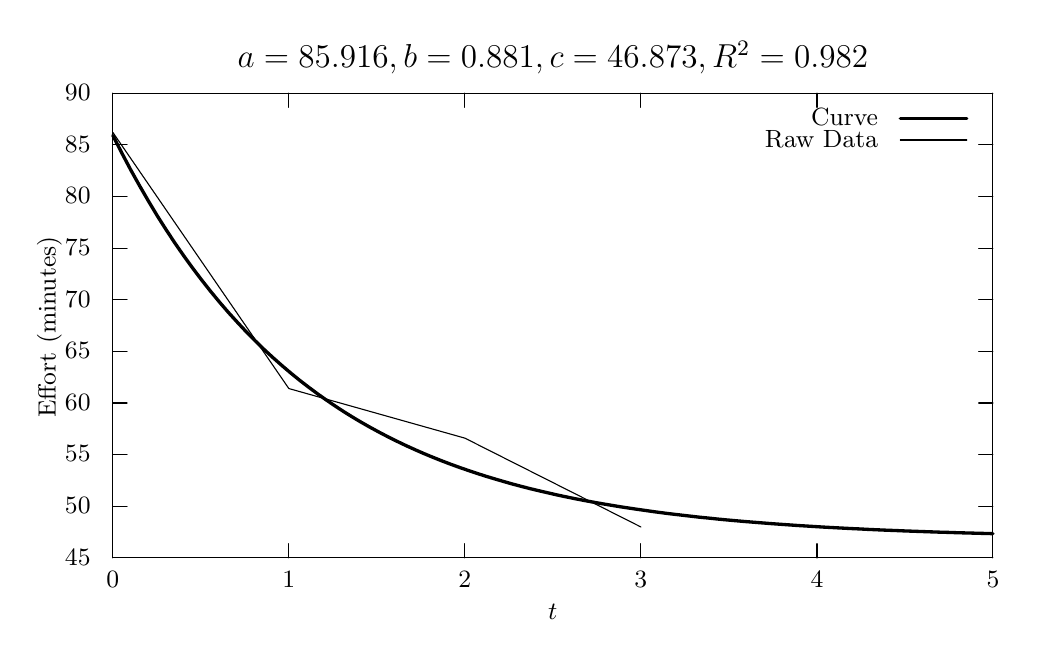
\begin{tikzpicture}[gnuplot]
%% generated with GNUPLOT 4.6p4 (Lua 5.1; terminal rev. 99, script rev. 100)
%% Fri 03 Oct 2014 12:39:55 WST
\tikzset{every node/.append style={font={\fontsize{9pt}{10.8pt}\selectfont}}}
\gpmonochromelines
\path (0.000,0.000) rectangle (12.700,7.620);
\gpcolor{color=gp lt color border}
\gpsetlinetype{gp lt border}
\gpsetlinewidth{1.00}
\draw[gp path] (1.024,0.886)--(1.204,0.886);
\draw[gp path] (12.201,0.886)--(12.021,0.886);
\node[gp node right] at (0.858,0.886) {45};
\draw[gp path] (1.024,1.542)--(1.204,1.542);
\draw[gp path] (12.201,1.542)--(12.021,1.542);
\node[gp node right] at (0.858,1.542) {50};
\draw[gp path] (1.024,2.198)--(1.204,2.198);
\draw[gp path] (12.201,2.198)--(12.021,2.198);
\node[gp node right] at (0.858,2.198) {55};
\draw[gp path] (1.024,2.853)--(1.204,2.853);
\draw[gp path] (12.201,2.853)--(12.021,2.853);
\node[gp node right] at (0.858,2.853) {60};
\draw[gp path] (1.024,3.509)--(1.204,3.509);
\draw[gp path] (12.201,3.509)--(12.021,3.509);
\node[gp node right] at (0.858,3.509) {65};
\draw[gp path] (1.024,4.165)--(1.204,4.165);
\draw[gp path] (12.201,4.165)--(12.021,4.165);
\node[gp node right] at (0.858,4.165) {70};
\draw[gp path] (1.024,4.821)--(1.204,4.821);
\draw[gp path] (12.201,4.821)--(12.021,4.821);
\node[gp node right] at (0.858,4.821) {75};
\draw[gp path] (1.024,5.476)--(1.204,5.476);
\draw[gp path] (12.201,5.476)--(12.021,5.476);
\node[gp node right] at (0.858,5.476) {80};
\draw[gp path] (1.024,6.132)--(1.204,6.132);
\draw[gp path] (12.201,6.132)--(12.021,6.132);
\node[gp node right] at (0.858,6.132) {85};
\draw[gp path] (1.024,6.788)--(1.204,6.788);
\draw[gp path] (12.201,6.788)--(12.021,6.788);
\node[gp node right] at (0.858,6.788) {90};
\draw[gp path] (1.024,0.886)--(1.024,1.066);
\draw[gp path] (1.024,6.788)--(1.024,6.608);
\node[gp node center] at (1.024,0.609) {0};
\draw[gp path] (3.259,0.886)--(3.259,1.066);
\draw[gp path] (3.259,6.788)--(3.259,6.608);
\node[gp node center] at (3.259,0.609) {1};
\draw[gp path] (5.495,0.886)--(5.495,1.066);
\draw[gp path] (5.495,6.788)--(5.495,6.608);
\node[gp node center] at (5.495,0.609) {2};
\draw[gp path] (7.730,0.886)--(7.730,1.066);
\draw[gp path] (7.730,6.788)--(7.730,6.608);
\node[gp node center] at (7.730,0.609) {3};
\draw[gp path] (9.966,0.886)--(9.966,1.066);
\draw[gp path] (9.966,6.788)--(9.966,6.608);
\node[gp node center] at (9.966,0.609) {4};
\draw[gp path] (12.201,0.886)--(12.201,1.066);
\draw[gp path] (12.201,6.788)--(12.201,6.608);
\node[gp node center] at (12.201,0.609) {5};
\draw[gp path] (1.024,6.788)--(1.024,0.886)--(12.201,0.886)--(12.201,6.788)--cycle;
\node[gp node center,rotate=-270] at (0.221,3.837) {Effort (minutes)};
\node[gp node center] at (6.612,0.194) {$t$};
\node[gp node center,font={\fontsize{12pt}{14.4pt}\selectfont}] at (6.612,7.204) {$a = 85.916, b = 0.881, c = 46.873, R^2 = 0.982$};
\node[gp node right] at (10.859,6.470) {Curve};
\gpcolor{color=gp lt color 0}
\gpsetlinetype{gp lt plot 0}
\gpsetlinewidth{3.00}
\draw[gp path] (11.025,6.470)--(11.869,6.470);
\draw[gp path] (1.024,6.252)--(1.137,6.030)--(1.250,5.816)--(1.363,5.613)--(1.476,5.418)%
  --(1.588,5.231)--(1.701,5.053)--(1.814,4.882)--(1.927,4.719)--(2.040,4.563)--(2.153,4.414)%
  --(2.266,4.271)--(2.379,4.134)--(2.492,4.003)--(2.605,3.879)--(2.717,3.759)--(2.830,3.645)%
  --(2.943,3.535)--(3.056,3.431)--(3.169,3.331)--(3.282,3.235)--(3.395,3.143)--(3.508,3.056)%
  --(3.621,2.972)--(3.734,2.892)--(3.846,2.816)--(3.959,2.742)--(4.072,2.672)--(4.185,2.605)%
  --(4.298,2.541)--(4.411,2.480)--(4.524,2.421)--(4.637,2.365)--(4.750,2.311)--(4.863,2.260)%
  --(4.975,2.211)--(5.088,2.164)--(5.201,2.119)--(5.314,2.076)--(5.427,2.035)--(5.540,1.996)%
  --(5.653,1.958)--(5.766,1.922)--(5.879,1.888)--(5.992,1.855)--(6.104,1.823)--(6.217,1.793)%
  --(6.330,1.764)--(6.443,1.737)--(6.556,1.711)--(6.669,1.685)--(6.782,1.661)--(6.895,1.638)%
  --(7.008,1.616)--(7.121,1.595)--(7.233,1.575)--(7.346,1.556)--(7.459,1.537)--(7.572,1.520)%
  --(7.685,1.503)--(7.798,1.487)--(7.911,1.471)--(8.024,1.456)--(8.137,1.442)--(8.250,1.429)%
  --(8.362,1.416)--(8.475,1.403)--(8.588,1.392)--(8.701,1.380)--(8.814,1.369)--(8.927,1.359)%
  --(9.040,1.349)--(9.153,1.340)--(9.266,1.331)--(9.379,1.322)--(9.491,1.314)--(9.604,1.306)%
  --(9.717,1.298)--(9.830,1.291)--(9.943,1.284)--(10.056,1.277)--(10.169,1.271)--(10.282,1.265)%
  --(10.395,1.259)--(10.508,1.254)--(10.620,1.248)--(10.733,1.243)--(10.846,1.238)--(10.959,1.234)%
  --(11.072,1.229)--(11.185,1.225)--(11.298,1.221)--(11.411,1.217)--(11.524,1.213)--(11.637,1.210)%
  --(11.749,1.206)--(11.862,1.203)--(11.975,1.200)--(12.088,1.197)--(12.201,1.194);
\gpcolor{color=gp lt color border}
\node[gp node right] at (10.859,6.193) {Raw Data};
\gpcolor{color=gp lt color 3}
\gpsetlinetype{gp lt plot 3}
\gpsetlinewidth{1.00}
\draw[gp path] (11.025,6.193)--(11.869,6.193);
\draw[gp path] (1.024,6.290)--(3.259,3.037)--(5.495,2.407)--(7.730,1.279);
\gpcolor{color=gp lt color border}
\gpsetlinetype{gp lt border}
\draw[gp path] (1.024,6.788)--(1.024,0.886)--(12.201,0.886)--(12.201,6.788)--cycle;
%% coordinates of the plot area
\gpdefrectangularnode{gp plot 1}{\pgfpoint{1.024cm}{0.886cm}}{\pgfpoint{12.201cm}{6.788cm}}
\end{tikzpicture}
%% gnuplot variables

  \caption{Problem 2 Language A}
  \end{figure}
  
  \begin{figure}[!htb]
  \centering
  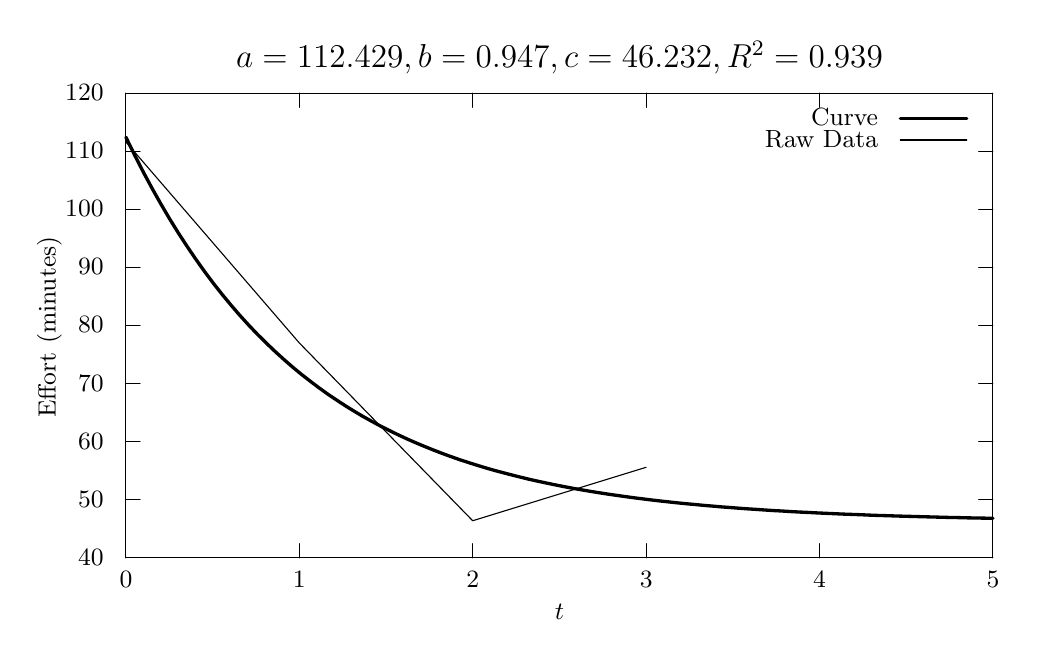
\begin{tikzpicture}[gnuplot]
%% generated with GNUPLOT 4.6p4 (Lua 5.1; terminal rev. 99, script rev. 100)
%% Fri 03 Oct 2014 12:39:55 WST
\tikzset{every node/.append style={font={\fontsize{9pt}{10.8pt}\selectfont}}}
\gpmonochromelines
\path (0.000,0.000) rectangle (12.700,7.620);
\gpcolor{color=gp lt color border}
\gpsetlinetype{gp lt border}
\gpsetlinewidth{1.00}
\draw[gp path] (1.190,0.886)--(1.370,0.886);
\draw[gp path] (12.201,0.886)--(12.021,0.886);
\node[gp node right] at (1.024,0.886) {40};
\draw[gp path] (1.190,1.624)--(1.370,1.624);
\draw[gp path] (12.201,1.624)--(12.021,1.624);
\node[gp node right] at (1.024,1.624) {50};
\draw[gp path] (1.190,2.362)--(1.370,2.362);
\draw[gp path] (12.201,2.362)--(12.021,2.362);
\node[gp node right] at (1.024,2.362) {60};
\draw[gp path] (1.190,3.099)--(1.370,3.099);
\draw[gp path] (12.201,3.099)--(12.021,3.099);
\node[gp node right] at (1.024,3.099) {70};
\draw[gp path] (1.190,3.837)--(1.370,3.837);
\draw[gp path] (12.201,3.837)--(12.021,3.837);
\node[gp node right] at (1.024,3.837) {80};
\draw[gp path] (1.190,4.575)--(1.370,4.575);
\draw[gp path] (12.201,4.575)--(12.021,4.575);
\node[gp node right] at (1.024,4.575) {90};
\draw[gp path] (1.190,5.313)--(1.370,5.313);
\draw[gp path] (12.201,5.313)--(12.021,5.313);
\node[gp node right] at (1.024,5.313) {100};
\draw[gp path] (1.190,6.050)--(1.370,6.050);
\draw[gp path] (12.201,6.050)--(12.021,6.050);
\node[gp node right] at (1.024,6.050) {110};
\draw[gp path] (1.190,6.788)--(1.370,6.788);
\draw[gp path] (12.201,6.788)--(12.021,6.788);
\node[gp node right] at (1.024,6.788) {120};
\draw[gp path] (1.190,0.886)--(1.190,1.066);
\draw[gp path] (1.190,6.788)--(1.190,6.608);
\node[gp node center] at (1.190,0.609) {0};
\draw[gp path] (3.392,0.886)--(3.392,1.066);
\draw[gp path] (3.392,6.788)--(3.392,6.608);
\node[gp node center] at (3.392,0.609) {1};
\draw[gp path] (5.594,0.886)--(5.594,1.066);
\draw[gp path] (5.594,6.788)--(5.594,6.608);
\node[gp node center] at (5.594,0.609) {2};
\draw[gp path] (7.797,0.886)--(7.797,1.066);
\draw[gp path] (7.797,6.788)--(7.797,6.608);
\node[gp node center] at (7.797,0.609) {3};
\draw[gp path] (9.999,0.886)--(9.999,1.066);
\draw[gp path] (9.999,6.788)--(9.999,6.608);
\node[gp node center] at (9.999,0.609) {4};
\draw[gp path] (12.201,0.886)--(12.201,1.066);
\draw[gp path] (12.201,6.788)--(12.201,6.608);
\node[gp node center] at (12.201,0.609) {5};
\draw[gp path] (1.190,6.788)--(1.190,0.886)--(12.201,0.886)--(12.201,6.788)--cycle;
\node[gp node center,rotate=-270] at (0.221,3.837) {Effort (minutes)};
\node[gp node center] at (6.695,0.194) {$t$};
\node[gp node center,font={\fontsize{12pt}{14.4pt}\selectfont}] at (6.695,7.204) {$a = 112.429, b = 0.947, c = 46.232, R^2 = 0.939$};
\node[gp node right] at (10.859,6.470) {Curve};
\gpcolor{color=gp lt color 0}
\gpsetlinetype{gp lt plot 0}
\gpsetlinewidth{3.00}
\draw[gp path] (11.025,6.470)--(11.869,6.470);
\draw[gp path] (1.190,6.229)--(1.301,6.001)--(1.412,5.784)--(1.524,5.576)--(1.635,5.379)%
  --(1.746,5.190)--(1.857,5.011)--(1.969,4.839)--(2.080,4.676)--(2.191,4.520)--(2.302,4.372)%
  --(2.413,4.231)--(2.525,4.096)--(2.636,3.967)--(2.747,3.845)--(2.858,3.728)--(2.970,3.617)%
  --(3.081,3.511)--(3.192,3.410)--(3.303,3.313)--(3.414,3.221)--(3.526,3.134)--(3.637,3.050)%
  --(3.748,2.970)--(3.859,2.895)--(3.971,2.822)--(4.082,2.753)--(4.193,2.687)--(4.304,2.625)%
  --(4.415,2.565)--(4.527,2.508)--(4.638,2.454)--(4.749,2.402)--(4.860,2.353)--(4.972,2.306)%
  --(5.083,2.261)--(5.194,2.218)--(5.305,2.177)--(5.416,2.138)--(5.528,2.101)--(5.639,2.066)%
  --(5.750,2.032)--(5.861,2.000)--(5.973,1.970)--(6.084,1.941)--(6.195,1.913)--(6.306,1.886)%
  --(6.417,1.861)--(6.529,1.837)--(6.640,1.814)--(6.751,1.792)--(6.862,1.771)--(6.974,1.751)%
  --(7.085,1.732)--(7.196,1.714)--(7.307,1.697)--(7.418,1.681)--(7.530,1.665)--(7.641,1.650)%
  --(7.752,1.636)--(7.863,1.622)--(7.975,1.609)--(8.086,1.597)--(8.197,1.585)--(8.308,1.574)%
  --(8.419,1.564)--(8.531,1.553)--(8.642,1.544)--(8.753,1.534)--(8.864,1.526)--(8.976,1.517)%
  --(9.087,1.509)--(9.198,1.502)--(9.309,1.494)--(9.420,1.487)--(9.532,1.481)--(9.643,1.474)%
  --(9.754,1.468)--(9.865,1.463)--(9.977,1.457)--(10.088,1.452)--(10.199,1.447)--(10.310,1.442)%
  --(10.421,1.438)--(10.533,1.434)--(10.644,1.429)--(10.755,1.425)--(10.866,1.422)--(10.978,1.418)%
  --(11.089,1.415)--(11.200,1.412)--(11.311,1.409)--(11.422,1.406)--(11.534,1.403)--(11.645,1.400)%
  --(11.756,1.398)--(11.867,1.395)--(11.979,1.393)--(12.090,1.391)--(12.201,1.389);
\gpcolor{color=gp lt color border}
\node[gp node right] at (10.859,6.193) {Raw Data};
\gpcolor{color=gp lt color 3}
\gpsetlinetype{gp lt plot 3}
\gpsetlinewidth{1.00}
\draw[gp path] (11.025,6.193)--(11.869,6.193);
\draw[gp path] (1.190,6.168)--(3.392,3.616)--(5.594,1.358)--(7.797,2.037);
\gpcolor{color=gp lt color border}
\gpsetlinetype{gp lt border}
\draw[gp path] (1.190,6.788)--(1.190,0.886)--(12.201,0.886)--(12.201,6.788)--cycle;
%% coordinates of the plot area
\gpdefrectangularnode{gp plot 1}{\pgfpoint{1.190cm}{0.886cm}}{\pgfpoint{12.201cm}{6.788cm}}
\end{tikzpicture}
%% gnuplot variables

  \caption{Problem 1 Language B}
  \end{figure}
  
  \FloatBarrier
  \subsection{Model D}
  $$a+bt+ct^2$$
  
  \begin{figure}[!htb]
  \centering
  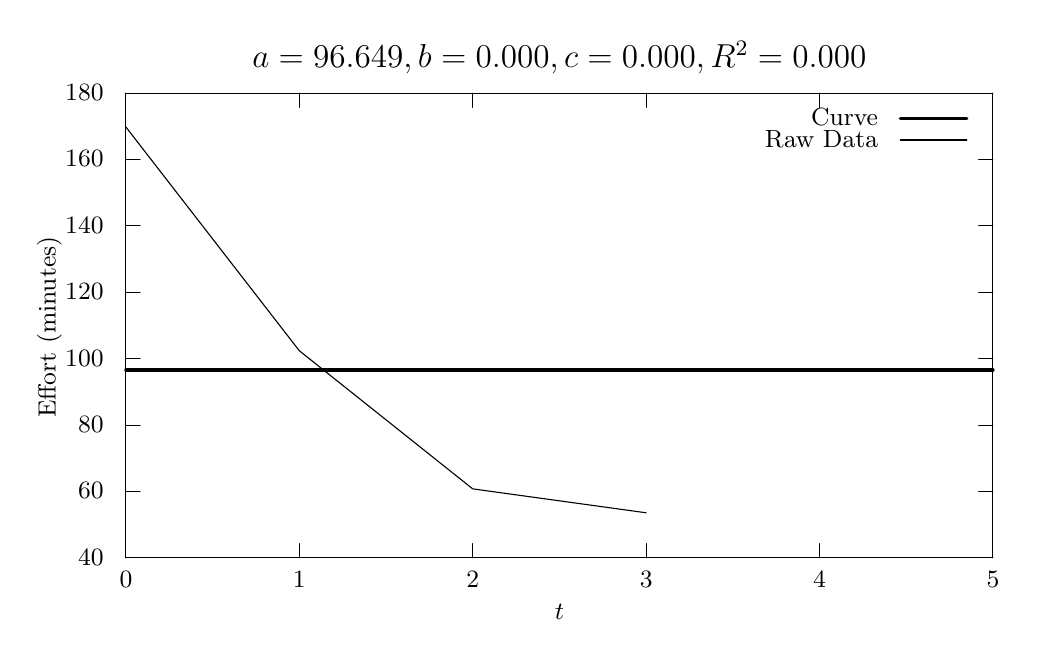
\begin{tikzpicture}[gnuplot]
%% generated with GNUPLOT 4.6p4 (Lua 5.1; terminal rev. 99, script rev. 100)
%% Fri 03 Oct 2014 12:39:55 WST
\tikzset{every node/.append style={font={\fontsize{9pt}{10.8pt}\selectfont}}}
\gpmonochromelines
\path (0.000,0.000) rectangle (12.700,7.620);
\gpcolor{color=gp lt color border}
\gpsetlinetype{gp lt border}
\gpsetlinewidth{1.00}
\draw[gp path] (1.190,0.886)--(1.370,0.886);
\draw[gp path] (12.201,0.886)--(12.021,0.886);
\node[gp node right] at (1.024,0.886) {40};
\draw[gp path] (1.190,1.729)--(1.370,1.729);
\draw[gp path] (12.201,1.729)--(12.021,1.729);
\node[gp node right] at (1.024,1.729) {60};
\draw[gp path] (1.190,2.572)--(1.370,2.572);
\draw[gp path] (12.201,2.572)--(12.021,2.572);
\node[gp node right] at (1.024,2.572) {80};
\draw[gp path] (1.190,3.415)--(1.370,3.415);
\draw[gp path] (12.201,3.415)--(12.021,3.415);
\node[gp node right] at (1.024,3.415) {100};
\draw[gp path] (1.190,4.259)--(1.370,4.259);
\draw[gp path] (12.201,4.259)--(12.021,4.259);
\node[gp node right] at (1.024,4.259) {120};
\draw[gp path] (1.190,5.102)--(1.370,5.102);
\draw[gp path] (12.201,5.102)--(12.021,5.102);
\node[gp node right] at (1.024,5.102) {140};
\draw[gp path] (1.190,5.945)--(1.370,5.945);
\draw[gp path] (12.201,5.945)--(12.021,5.945);
\node[gp node right] at (1.024,5.945) {160};
\draw[gp path] (1.190,6.788)--(1.370,6.788);
\draw[gp path] (12.201,6.788)--(12.021,6.788);
\node[gp node right] at (1.024,6.788) {180};
\draw[gp path] (1.190,0.886)--(1.190,1.066);
\draw[gp path] (1.190,6.788)--(1.190,6.608);
\node[gp node center] at (1.190,0.609) {0};
\draw[gp path] (3.392,0.886)--(3.392,1.066);
\draw[gp path] (3.392,6.788)--(3.392,6.608);
\node[gp node center] at (3.392,0.609) {1};
\draw[gp path] (5.594,0.886)--(5.594,1.066);
\draw[gp path] (5.594,6.788)--(5.594,6.608);
\node[gp node center] at (5.594,0.609) {2};
\draw[gp path] (7.797,0.886)--(7.797,1.066);
\draw[gp path] (7.797,6.788)--(7.797,6.608);
\node[gp node center] at (7.797,0.609) {3};
\draw[gp path] (9.999,0.886)--(9.999,1.066);
\draw[gp path] (9.999,6.788)--(9.999,6.608);
\node[gp node center] at (9.999,0.609) {4};
\draw[gp path] (12.201,0.886)--(12.201,1.066);
\draw[gp path] (12.201,6.788)--(12.201,6.608);
\node[gp node center] at (12.201,0.609) {5};
\draw[gp path] (1.190,6.788)--(1.190,0.886)--(12.201,0.886)--(12.201,6.788)--cycle;
\node[gp node center,rotate=-270] at (0.221,3.837) {Effort (minutes)};
\node[gp node center] at (6.695,0.194) {$t$};
\node[gp node center,font={\fontsize{12pt}{14.4pt}\selectfont}] at (6.695,7.204) {$a = 96.649, b = 0.000, c = 0.000, R^2 = 0.000$};
\node[gp node right] at (10.859,6.470) {Curve};
\gpcolor{color=gp lt color 0}
\gpsetlinetype{gp lt plot 0}
\gpsetlinewidth{3.00}
\draw[gp path] (11.025,6.470)--(11.869,6.470);
\draw[gp path] (1.190,3.274)--(1.301,3.274)--(1.412,3.274)--(1.524,3.274)--(1.635,3.274)%
  --(1.746,3.274)--(1.857,3.274)--(1.969,3.274)--(2.080,3.274)--(2.191,3.274)--(2.302,3.274)%
  --(2.413,3.274)--(2.525,3.274)--(2.636,3.274)--(2.747,3.274)--(2.858,3.274)--(2.970,3.274)%
  --(3.081,3.274)--(3.192,3.274)--(3.303,3.274)--(3.414,3.274)--(3.526,3.274)--(3.637,3.274)%
  --(3.748,3.274)--(3.859,3.274)--(3.971,3.274)--(4.082,3.274)--(4.193,3.274)--(4.304,3.274)%
  --(4.415,3.274)--(4.527,3.274)--(4.638,3.274)--(4.749,3.274)--(4.860,3.274)--(4.972,3.274)%
  --(5.083,3.274)--(5.194,3.274)--(5.305,3.274)--(5.416,3.274)--(5.528,3.274)--(5.639,3.274)%
  --(5.750,3.274)--(5.861,3.274)--(5.973,3.274)--(6.084,3.274)--(6.195,3.274)--(6.306,3.274)%
  --(6.417,3.274)--(6.529,3.274)--(6.640,3.274)--(6.751,3.274)--(6.862,3.274)--(6.974,3.274)%
  --(7.085,3.274)--(7.196,3.274)--(7.307,3.274)--(7.418,3.274)--(7.530,3.274)--(7.641,3.274)%
  --(7.752,3.274)--(7.863,3.274)--(7.975,3.274)--(8.086,3.274)--(8.197,3.274)--(8.308,3.274)%
  --(8.419,3.274)--(8.531,3.274)--(8.642,3.274)--(8.753,3.274)--(8.864,3.274)--(8.976,3.274)%
  --(9.087,3.274)--(9.198,3.274)--(9.309,3.274)--(9.420,3.274)--(9.532,3.274)--(9.643,3.274)%
  --(9.754,3.274)--(9.865,3.274)--(9.977,3.274)--(10.088,3.274)--(10.199,3.274)--(10.310,3.274)%
  --(10.421,3.274)--(10.533,3.274)--(10.644,3.274)--(10.755,3.274)--(10.866,3.274)--(10.978,3.274)%
  --(11.089,3.274)--(11.200,3.274)--(11.311,3.274)--(11.422,3.274)--(11.534,3.274)--(11.645,3.274)%
  --(11.756,3.274)--(11.867,3.274)--(11.979,3.274)--(12.090,3.274)--(12.201,3.274);
\gpcolor{color=gp lt color border}
\node[gp node right] at (10.859,6.193) {Raw Data};
\gpcolor{color=gp lt color 3}
\gpsetlinetype{gp lt plot 3}
\gpsetlinewidth{1.00}
\draw[gp path] (11.025,6.193)--(11.869,6.193);
\draw[gp path] (1.190,6.358)--(3.392,3.517)--(5.594,1.763)--(7.797,1.459);
\gpcolor{color=gp lt color border}
\gpsetlinetype{gp lt border}
\draw[gp path] (1.190,6.788)--(1.190,0.886)--(12.201,0.886)--(12.201,6.788)--cycle;
%% coordinates of the plot area
\gpdefrectangularnode{gp plot 1}{\pgfpoint{1.190cm}{0.886cm}}{\pgfpoint{12.201cm}{6.788cm}}
\end{tikzpicture}
%% gnuplot variables

  \caption{Problem 1 Language A}
  \end{figure}
  
  \begin{figure}[!htb]
  \centering
  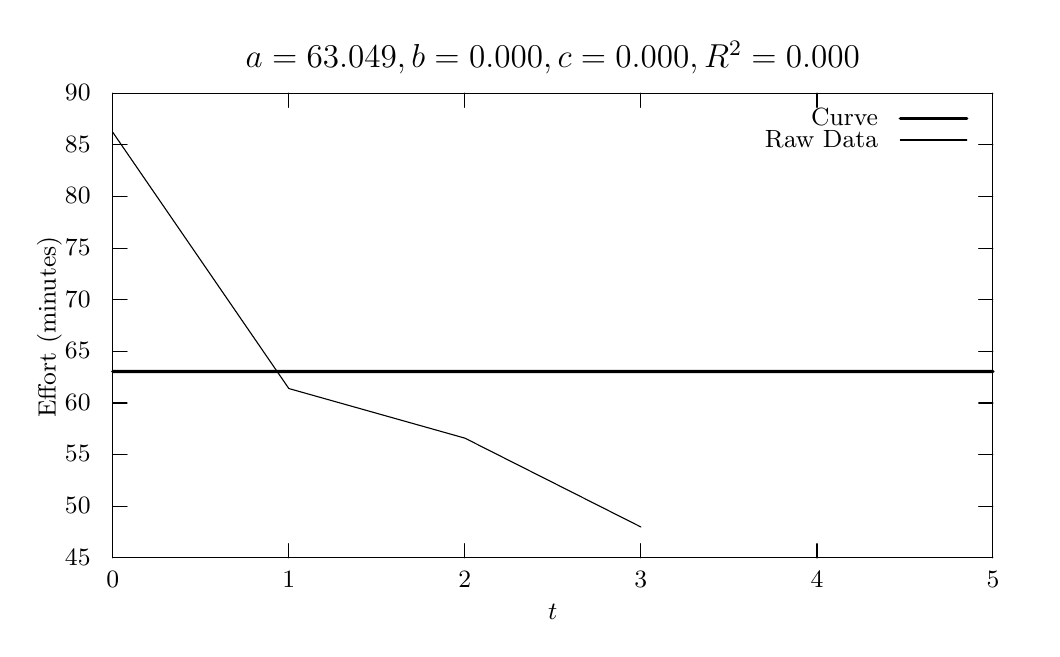
\begin{tikzpicture}[gnuplot]
%% generated with GNUPLOT 4.6p4 (Lua 5.1; terminal rev. 99, script rev. 100)
%% Fri 03 Oct 2014 12:39:55 WST
\tikzset{every node/.append style={font={\fontsize{9pt}{10.8pt}\selectfont}}}
\gpmonochromelines
\path (0.000,0.000) rectangle (12.700,7.620);
\gpcolor{color=gp lt color border}
\gpsetlinetype{gp lt border}
\gpsetlinewidth{1.00}
\draw[gp path] (1.024,0.886)--(1.204,0.886);
\draw[gp path] (12.201,0.886)--(12.021,0.886);
\node[gp node right] at (0.858,0.886) {45};
\draw[gp path] (1.024,1.542)--(1.204,1.542);
\draw[gp path] (12.201,1.542)--(12.021,1.542);
\node[gp node right] at (0.858,1.542) {50};
\draw[gp path] (1.024,2.198)--(1.204,2.198);
\draw[gp path] (12.201,2.198)--(12.021,2.198);
\node[gp node right] at (0.858,2.198) {55};
\draw[gp path] (1.024,2.853)--(1.204,2.853);
\draw[gp path] (12.201,2.853)--(12.021,2.853);
\node[gp node right] at (0.858,2.853) {60};
\draw[gp path] (1.024,3.509)--(1.204,3.509);
\draw[gp path] (12.201,3.509)--(12.021,3.509);
\node[gp node right] at (0.858,3.509) {65};
\draw[gp path] (1.024,4.165)--(1.204,4.165);
\draw[gp path] (12.201,4.165)--(12.021,4.165);
\node[gp node right] at (0.858,4.165) {70};
\draw[gp path] (1.024,4.821)--(1.204,4.821);
\draw[gp path] (12.201,4.821)--(12.021,4.821);
\node[gp node right] at (0.858,4.821) {75};
\draw[gp path] (1.024,5.476)--(1.204,5.476);
\draw[gp path] (12.201,5.476)--(12.021,5.476);
\node[gp node right] at (0.858,5.476) {80};
\draw[gp path] (1.024,6.132)--(1.204,6.132);
\draw[gp path] (12.201,6.132)--(12.021,6.132);
\node[gp node right] at (0.858,6.132) {85};
\draw[gp path] (1.024,6.788)--(1.204,6.788);
\draw[gp path] (12.201,6.788)--(12.021,6.788);
\node[gp node right] at (0.858,6.788) {90};
\draw[gp path] (1.024,0.886)--(1.024,1.066);
\draw[gp path] (1.024,6.788)--(1.024,6.608);
\node[gp node center] at (1.024,0.609) {0};
\draw[gp path] (3.259,0.886)--(3.259,1.066);
\draw[gp path] (3.259,6.788)--(3.259,6.608);
\node[gp node center] at (3.259,0.609) {1};
\draw[gp path] (5.495,0.886)--(5.495,1.066);
\draw[gp path] (5.495,6.788)--(5.495,6.608);
\node[gp node center] at (5.495,0.609) {2};
\draw[gp path] (7.730,0.886)--(7.730,1.066);
\draw[gp path] (7.730,6.788)--(7.730,6.608);
\node[gp node center] at (7.730,0.609) {3};
\draw[gp path] (9.966,0.886)--(9.966,1.066);
\draw[gp path] (9.966,6.788)--(9.966,6.608);
\node[gp node center] at (9.966,0.609) {4};
\draw[gp path] (12.201,0.886)--(12.201,1.066);
\draw[gp path] (12.201,6.788)--(12.201,6.608);
\node[gp node center] at (12.201,0.609) {5};
\draw[gp path] (1.024,6.788)--(1.024,0.886)--(12.201,0.886)--(12.201,6.788)--cycle;
\node[gp node center,rotate=-270] at (0.221,3.837) {Effort (minutes)};
\node[gp node center] at (6.612,0.194) {$t$};
\node[gp node center,font={\fontsize{12pt}{14.4pt}\selectfont}] at (6.612,7.204) {$a = 63.049, b = 0.000, c = 0.000, R^2 = 0.000$};
\node[gp node right] at (10.859,6.470) {Curve};
\gpcolor{color=gp lt color 0}
\gpsetlinetype{gp lt plot 0}
\gpsetlinewidth{3.00}
\draw[gp path] (11.025,6.470)--(11.869,6.470);
\draw[gp path] (1.024,3.253)--(1.137,3.253)--(1.250,3.253)--(1.363,3.253)--(1.476,3.253)%
  --(1.588,3.253)--(1.701,3.253)--(1.814,3.253)--(1.927,3.253)--(2.040,3.253)--(2.153,3.253)%
  --(2.266,3.253)--(2.379,3.253)--(2.492,3.253)--(2.605,3.253)--(2.717,3.253)--(2.830,3.253)%
  --(2.943,3.253)--(3.056,3.253)--(3.169,3.253)--(3.282,3.253)--(3.395,3.253)--(3.508,3.253)%
  --(3.621,3.253)--(3.734,3.253)--(3.846,3.253)--(3.959,3.253)--(4.072,3.253)--(4.185,3.253)%
  --(4.298,3.253)--(4.411,3.253)--(4.524,3.253)--(4.637,3.253)--(4.750,3.253)--(4.863,3.253)%
  --(4.975,3.253)--(5.088,3.253)--(5.201,3.253)--(5.314,3.253)--(5.427,3.253)--(5.540,3.253)%
  --(5.653,3.253)--(5.766,3.253)--(5.879,3.253)--(5.992,3.253)--(6.104,3.253)--(6.217,3.253)%
  --(6.330,3.253)--(6.443,3.253)--(6.556,3.253)--(6.669,3.253)--(6.782,3.253)--(6.895,3.253)%
  --(7.008,3.253)--(7.121,3.253)--(7.233,3.253)--(7.346,3.253)--(7.459,3.253)--(7.572,3.253)%
  --(7.685,3.253)--(7.798,3.253)--(7.911,3.253)--(8.024,3.253)--(8.137,3.253)--(8.250,3.253)%
  --(8.362,3.253)--(8.475,3.253)--(8.588,3.253)--(8.701,3.253)--(8.814,3.253)--(8.927,3.254)%
  --(9.040,3.254)--(9.153,3.254)--(9.266,3.254)--(9.379,3.254)--(9.491,3.254)--(9.604,3.254)%
  --(9.717,3.254)--(9.830,3.254)--(9.943,3.254)--(10.056,3.254)--(10.169,3.254)--(10.282,3.254)%
  --(10.395,3.254)--(10.508,3.254)--(10.620,3.254)--(10.733,3.254)--(10.846,3.254)--(10.959,3.254)%
  --(11.072,3.254)--(11.185,3.254)--(11.298,3.254)--(11.411,3.254)--(11.524,3.254)--(11.637,3.254)%
  --(11.749,3.254)--(11.862,3.254)--(11.975,3.254)--(12.088,3.254)--(12.201,3.254);
\gpcolor{color=gp lt color border}
\node[gp node right] at (10.859,6.193) {Raw Data};
\gpcolor{color=gp lt color 3}
\gpsetlinetype{gp lt plot 3}
\gpsetlinewidth{1.00}
\draw[gp path] (11.025,6.193)--(11.869,6.193);
\draw[gp path] (1.024,6.290)--(3.259,3.037)--(5.495,2.407)--(7.730,1.279);
\gpcolor{color=gp lt color border}
\gpsetlinetype{gp lt border}
\draw[gp path] (1.024,6.788)--(1.024,0.886)--(12.201,0.886)--(12.201,6.788)--cycle;
%% coordinates of the plot area
\gpdefrectangularnode{gp plot 1}{\pgfpoint{1.024cm}{0.886cm}}{\pgfpoint{12.201cm}{6.788cm}}
\end{tikzpicture}
%% gnuplot variables

  \caption{Problem 2 Language A}
  \end{figure}
  
  \begin{figure}[!htb]
  \centering
  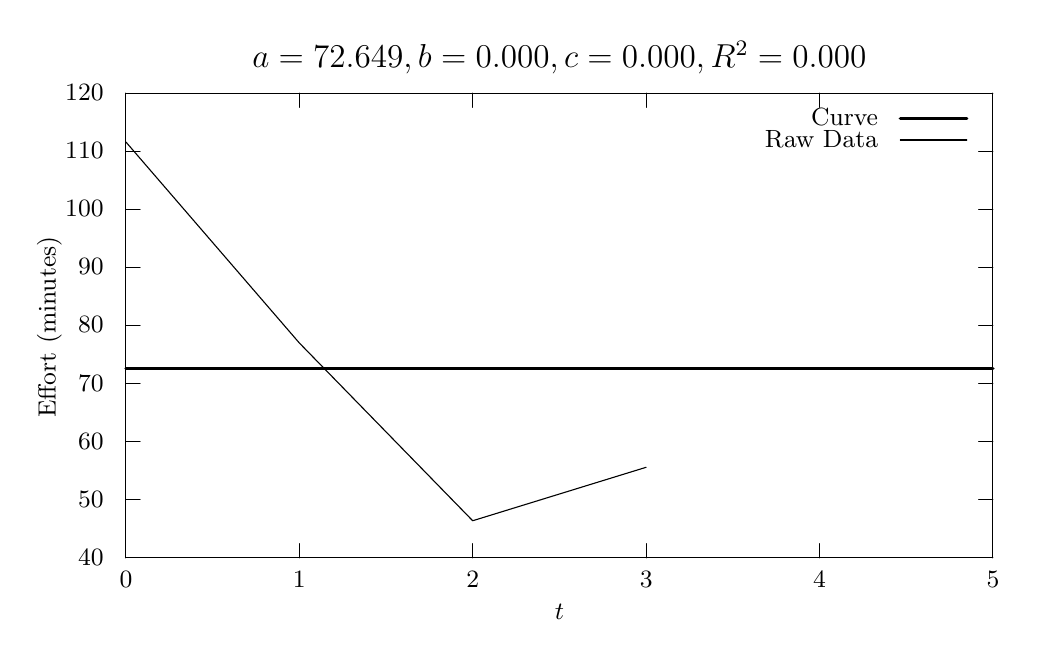
\begin{tikzpicture}[gnuplot]
%% generated with GNUPLOT 4.6p4 (Lua 5.1; terminal rev. 99, script rev. 100)
%% Fri 03 Oct 2014 12:39:55 WST
\tikzset{every node/.append style={font={\fontsize{9pt}{10.8pt}\selectfont}}}
\gpmonochromelines
\path (0.000,0.000) rectangle (12.700,7.620);
\gpcolor{color=gp lt color border}
\gpsetlinetype{gp lt border}
\gpsetlinewidth{1.00}
\draw[gp path] (1.190,0.886)--(1.370,0.886);
\draw[gp path] (12.201,0.886)--(12.021,0.886);
\node[gp node right] at (1.024,0.886) {40};
\draw[gp path] (1.190,1.624)--(1.370,1.624);
\draw[gp path] (12.201,1.624)--(12.021,1.624);
\node[gp node right] at (1.024,1.624) {50};
\draw[gp path] (1.190,2.362)--(1.370,2.362);
\draw[gp path] (12.201,2.362)--(12.021,2.362);
\node[gp node right] at (1.024,2.362) {60};
\draw[gp path] (1.190,3.099)--(1.370,3.099);
\draw[gp path] (12.201,3.099)--(12.021,3.099);
\node[gp node right] at (1.024,3.099) {70};
\draw[gp path] (1.190,3.837)--(1.370,3.837);
\draw[gp path] (12.201,3.837)--(12.021,3.837);
\node[gp node right] at (1.024,3.837) {80};
\draw[gp path] (1.190,4.575)--(1.370,4.575);
\draw[gp path] (12.201,4.575)--(12.021,4.575);
\node[gp node right] at (1.024,4.575) {90};
\draw[gp path] (1.190,5.313)--(1.370,5.313);
\draw[gp path] (12.201,5.313)--(12.021,5.313);
\node[gp node right] at (1.024,5.313) {100};
\draw[gp path] (1.190,6.050)--(1.370,6.050);
\draw[gp path] (12.201,6.050)--(12.021,6.050);
\node[gp node right] at (1.024,6.050) {110};
\draw[gp path] (1.190,6.788)--(1.370,6.788);
\draw[gp path] (12.201,6.788)--(12.021,6.788);
\node[gp node right] at (1.024,6.788) {120};
\draw[gp path] (1.190,0.886)--(1.190,1.066);
\draw[gp path] (1.190,6.788)--(1.190,6.608);
\node[gp node center] at (1.190,0.609) {0};
\draw[gp path] (3.392,0.886)--(3.392,1.066);
\draw[gp path] (3.392,6.788)--(3.392,6.608);
\node[gp node center] at (3.392,0.609) {1};
\draw[gp path] (5.594,0.886)--(5.594,1.066);
\draw[gp path] (5.594,6.788)--(5.594,6.608);
\node[gp node center] at (5.594,0.609) {2};
\draw[gp path] (7.797,0.886)--(7.797,1.066);
\draw[gp path] (7.797,6.788)--(7.797,6.608);
\node[gp node center] at (7.797,0.609) {3};
\draw[gp path] (9.999,0.886)--(9.999,1.066);
\draw[gp path] (9.999,6.788)--(9.999,6.608);
\node[gp node center] at (9.999,0.609) {4};
\draw[gp path] (12.201,0.886)--(12.201,1.066);
\draw[gp path] (12.201,6.788)--(12.201,6.608);
\node[gp node center] at (12.201,0.609) {5};
\draw[gp path] (1.190,6.788)--(1.190,0.886)--(12.201,0.886)--(12.201,6.788)--cycle;
\node[gp node center,rotate=-270] at (0.221,3.837) {Effort (minutes)};
\node[gp node center] at (6.695,0.194) {$t$};
\node[gp node center,font={\fontsize{12pt}{14.4pt}\selectfont}] at (6.695,7.204) {$a = 72.649, b = 0.000, c = 0.000, R^2 = 0.000$};
\node[gp node right] at (10.859,6.470) {Curve};
\gpcolor{color=gp lt color 0}
\gpsetlinetype{gp lt plot 0}
\gpsetlinewidth{3.00}
\draw[gp path] (11.025,6.470)--(11.869,6.470);
\draw[gp path] (1.190,3.295)--(1.301,3.295)--(1.412,3.295)--(1.524,3.295)--(1.635,3.295)%
  --(1.746,3.295)--(1.857,3.295)--(1.969,3.295)--(2.080,3.295)--(2.191,3.295)--(2.302,3.295)%
  --(2.413,3.295)--(2.525,3.295)--(2.636,3.295)--(2.747,3.295)--(2.858,3.295)--(2.970,3.295)%
  --(3.081,3.295)--(3.192,3.295)--(3.303,3.295)--(3.414,3.295)--(3.526,3.295)--(3.637,3.295)%
  --(3.748,3.295)--(3.859,3.295)--(3.971,3.295)--(4.082,3.295)--(4.193,3.295)--(4.304,3.295)%
  --(4.415,3.295)--(4.527,3.295)--(4.638,3.295)--(4.749,3.295)--(4.860,3.295)--(4.972,3.295)%
  --(5.083,3.295)--(5.194,3.295)--(5.305,3.295)--(5.416,3.295)--(5.528,3.295)--(5.639,3.295)%
  --(5.750,3.295)--(5.861,3.295)--(5.973,3.295)--(6.084,3.295)--(6.195,3.295)--(6.306,3.295)%
  --(6.417,3.295)--(6.529,3.295)--(6.640,3.295)--(6.751,3.295)--(6.862,3.295)--(6.974,3.295)%
  --(7.085,3.295)--(7.196,3.295)--(7.307,3.295)--(7.418,3.295)--(7.530,3.295)--(7.641,3.295)%
  --(7.752,3.295)--(7.863,3.295)--(7.975,3.295)--(8.086,3.295)--(8.197,3.295)--(8.308,3.295)%
  --(8.419,3.295)--(8.531,3.295)--(8.642,3.295)--(8.753,3.295)--(8.864,3.295)--(8.976,3.295)%
  --(9.087,3.295)--(9.198,3.295)--(9.309,3.295)--(9.420,3.295)--(9.532,3.295)--(9.643,3.295)%
  --(9.754,3.295)--(9.865,3.295)--(9.977,3.295)--(10.088,3.295)--(10.199,3.295)--(10.310,3.295)%
  --(10.421,3.295)--(10.533,3.295)--(10.644,3.295)--(10.755,3.295)--(10.866,3.295)--(10.978,3.295)%
  --(11.089,3.295)--(11.200,3.295)--(11.311,3.295)--(11.422,3.295)--(11.534,3.295)--(11.645,3.295)%
  --(11.756,3.295)--(11.867,3.295)--(11.979,3.295)--(12.090,3.295)--(12.201,3.295);
\gpcolor{color=gp lt color border}
\node[gp node right] at (10.859,6.193) {Raw Data};
\gpcolor{color=gp lt color 3}
\gpsetlinetype{gp lt plot 3}
\gpsetlinewidth{1.00}
\draw[gp path] (11.025,6.193)--(11.869,6.193);
\draw[gp path] (1.190,6.168)--(3.392,3.616)--(5.594,1.358)--(7.797,2.037);
\gpcolor{color=gp lt color border}
\gpsetlinetype{gp lt border}
\draw[gp path] (1.190,6.788)--(1.190,0.886)--(12.201,0.886)--(12.201,6.788)--cycle;
%% coordinates of the plot area
\gpdefrectangularnode{gp plot 1}{\pgfpoint{1.190cm}{0.886cm}}{\pgfpoint{12.201cm}{6.788cm}}
\end{tikzpicture}
%% gnuplot variables

  \caption{Problem 1 Language B}
  \end{figure}
  
  \clearpage
  \section{Graph Generation Code}
  \label{sec:graphgencode}
  \begin{lstlisting}[language=Matlab]
% Written for Matlab. Outputs GnuPlot files which produce LaTeX figures.

% createFit.m
function [as, bs, cs, rsqs] = createFit(prefix, dataX, dataY, init)
eqs = char({'(a+b*c*x)/(b*x+1)',  '(a-c)*(x+1)^(-b)+c', ...
        '(a-c)*exp(-b*x)+c',  'a+b*x+c*x^2'});

eqs_gp = char({'(a+b*c*x)/(b*x+1)',  '(a-c)*(x+1)**(-b)+c', ...
        '(a-c)*exp(-b*x)+c',  'a+b*x+c*x**2'});

sze = size(dataY);
data = [dataX, dataY];
dlmwrite(strcat(prefix, '-data.txt'), data, '\t');
      
as = zeros(4, sze(2));
bs = zeros(4, sze(2));
cs = zeros(4, sze(2));

rsqs = zeros(4, sze(2));

for i=1:4,
  for j=1:sze(2),
    [xData, yData] = prepareCurveData(dataX, dataY(1:end,j));

    % Set up fittype and options.
    ft = fittype( eqs(i,1:end), 'independent', 'x', 'dependent', 'y' );
    opts = fitoptions( ft );
    opts.Display = 'Off';
    opts.Lower = [0.0002, 0.0001, 0.0001];
    opts.StartPoint = init;
    opts.Upper = [Inf Inf Inf];

    % Fit model to data.
    [fitresult, gof] = fit( xData, yData, ft, opts );
    rsq = gof.rsquare;
    indx = coeffnames(fitresult);
    vals = coeffvalues(fitresult);
    
    a = vals(find(ismember(indx,'a')));
    b = vals(find(ismember(indx,'b')));
    c = vals(find(ismember(indx,'c')));
    
    if rsq < 0
      rsq = 0;
    end
    
    as(i,j) = a;
    bs(i,j) = b;
    cs(i,j) = c;
    rsqs(i,j) = rsq;

    fp = fopen(strcat(prefix, '-plot', int2str(i), '-', int2str(j), '.p'), 'w');
    
    fprintf(fp, 'set term tikz monochrome dashed size 5in,3in font ",9"\n');
    fprintf(fp, 'set style func linespoints\n');
    fprintf(fp, 'set style data lines\n');
    fprintf(fp, 'set nogrid\n');
    fprintf(fp, 'set xrange [0:5]\n');
    fprintf(fp, 'set xlabel "$t$"\n');
    fprintf(fp, 'set ylabel "Effort (minutes)"\n');
    fprintf(fp, 'set title "$a = %.3f, b = %.3f, c = %.3f, R^2 = %.3f$"\n', ...
                    a, b, c, rsq);
    fprintf(fp, 'set title font ",12"\n');
    fprintf(fp, 'set format xy "%%g"\n');
    fprintf(fp, 'set output "%s-plot%d-%d.tex"\n', prefix, i, j);
    fprintf(fp, 'a = %f\n', a);
    fprintf(fp, 'b = %f\n', b);
    fprintf(fp, 'c = %f\n', c);
    fprintf(fp, 'f(x) = %s\n', eqs_gp(i,1:end));
    fprintf(fp, 'plot f(x) lw 3 lt 1 smooth csplines title "Curve", ');
    fprintf(fp, '"%s" using 1:%d lw 1 lt 4  title "Raw Data"\n', ...
                    strcat(prefix, '-data.txt'), j+1);
    fprintf(fp, 'set output\n');
    fprintf(fp, 'unset ylabel\n');
    fprintf(fp, 'unset xlabel\n');
    
    fclose(fp);
  end
end
end

% est.m
data1 = [169.8, 102.4, 60.8, 53.6;
	  86.2, 61.4, 56.6, 48;
	  111.6, 77, 46.4, 55.6].';
    
data2 = [90; 44; 461; 25];
data3 = [90; 44; 25];
    
dataX = [0; 1; 2; 3];

dataX2 = [0; 1; 3];

[a,b,c,r] = createFit('other', dataX, data1, [0.1321 0.7227 0.1104])
[a,b,c,r] = createFit('myincl', dataX, data2, [0.7232 0.3474 0.6606])
[a,b,c,r] = createFit('myexcl', dataX2, data3, [0.7232 0.3474 0.6606])
  \end{lstlisting}

  \clearpage
  \FloatBarrier
  \section{Programs}
  \label{sec:programs}
  
  \subsection{Raw Timings}
  \begin{table}[htb!]
    \centering
    \begin{tabular}{|r|rrrr|}
    \cline{2-5}
  \multicolumn{1}{c|}{} & \multicolumn{4}{|c|}{Program}  \\ 
  \multicolumn{1}{c|}{} & 1 & 2 & 3 & 4 \\ \hline
  Code & 57 & 19 & 46 & 11 \\
  Test/Fix & 26 & 15 & 210 & 9 \\
  Refactor & 7 & 10 & 13 & 2 \\
  Gather & 15 & 10 & 180 & 3 \\
  Design & 0 & 0 & 12 & 0 \\ \hline
  Total & 105 & 54 & 461 & 25 \\ \hline
    \end{tabular}
    \caption{Raw Timings}
    \label{tab:rawtimings}
  \end{table}
  
  \begin{table}[htb!]
   \centering
   \begin{tabular}{|l|l|}
    \hline
    Category & Maps to \\ \hline
    Knowledge Acquisition & Gather \\
    Solution Definition & Design, Refactor \\
    Knowledge Encoding & Code \\
    Solution Validation & Test/Fix \\ \hline
   \end{tabular}
    \caption{Categorising phases}
    \label{tab:rawtimingstocats}
  \end{table}
  
  \subsection{Program 0: Distance}
  \begin{lstlisting}[language=Python]
# Written for Python 3.4
# Output:
# Distance calculations!
#
# Distance from perth to uwa
#  = 4.287899604948252
#
# Distance from perth to greenwich
#  = 14485.978495782614
#
# Distance from perth to southpole
#  = 6715.917481245382
#
# Distance from uwa to greenwich
#  = 14485.767563601663
#
# Distance from uwa to southpole
#  = 6712.656749767587
#
# Distance from greenwich to southpole
#  = 15192.844590121906

from decimal import *
from math import radians
import itertools

# In degrees
PLACES = {
  #'uwa':        ('-31.981179', '115.81991'),
  #'perth':      ('-31.954265', '115.8523935'),
  #'greenwich':  ('51.4825766', '-0.0076589'),
  #'southpole':  ('-85', '0'),
  #'mackay':     ('-21.141857', '149.1829713'),
  'unihall':    ('-31.974053', '115.819057'),
  'darwin':     ('-12.5948609','131.0078759'),
  'melbourne':  ('-37.8602828','145.079616'),
}

RADIUS_EARTH = 6378



# Uses the Haversine formula
# Assumes spherical earth and radian coordinates
def distance(coord1, coord2):
  from math import asin, sqrt, cos, sin

  (lat1, long1), (lat2, long2) = coord1, coord2

  def haversin(v):
    return (sin(v/2))**2

  return 2 * RADIUS_EARTH * asin(
      sqrt(
        haversin(lat2 - lat1) + 
        cos(lat1) * cos(lat2) * haversin(long2 - long1)
      )
    )



if __name__ == "__main__":
  # Convert string coords into Decimal radian objects
  conv_places = {
    x : ( radians(Decimal(y1)), radians(Decimal(y2)) ) 
    for x, (y1, y2) in PLACES.items()
  }

  print('Distance calculations!')
  print()

  # Iterate over all place combinations and print the answers
  for (n1, c1), (n2, c2) in itertools.combinations(conv_places.items(), 2):

    print('Distance from {} to {}'.format(n1, n2))
    print('  = {}'.format(distance(c1, c2)))
    print()
  \end{lstlisting}
  
  \clearpage
  \subsection{Program 1: Area}
  \begin{lstlisting}[language=Python]
# Written for Python 3.4
# Output: 
# Calculating the area of ('unihall', 'darwin', 'melbourne')
# Distance between unihall and darwin
#  = 2657.806808418724
# Distance between darwin and melbourne
#  = 3140.2840494728316
# Distance between melbourne and unihall
#  = 2737.824326481584
# Area between points
#  = 3443496.4985877923


PLACES = {
  'unihall':    (-31.974053, 115.819057),
  'darwin':     (-12.5948609,131.0078759),
  'melbourne':  (-37.8602828,145.079616),
}

AREAS = [
  ('unihall', 'darwin', 'melbourne'),
]

RADIUS_EARTH = 6378

# From https://docs.python.org/3.1/library/itertools.html#recipes
def pairwise(iterable):
  "s -> (s0,s1), (s1,s2), (s2, s3), ..."
  from itertools import tee
  a, b = tee(iterable)
  next(b, None)
  return zip(a, b)


# Uses the Haversine formula, accepting lats/longs in radians
def dist(c1, c2):
  from math import sin, cos, asin, sqrt

  def haversin(v):
    return (1 - cos(v)) / 2

  (lat1, long1), (lat2, long2) = c1, c2

  return 2 * RADIUS_EARTH * asin(sqrt(
    haversin(lat2 - lat1) + 
    cos(lat1) * cos(lat2) * haversin(long2 - long1)
  ))

# Converts coordinate pair from degrees to radians
def coord_radians(c):
  from math import radians
  c1, c2 = c
  return (radians(c1), radians(c2))

# Calculates area of triange
def area(l1, l2, l3):
  from math import sqrt

  p = (l1 + l2 + l3) / 2
  return sqrt(p * (p - l1) * (p - l2) * (p - l3))



if __name__ == "__main__":
  # Convert the degrees to radians
  rplaces = {
    x : coord_radians(y) for (x, y) in PLACES.items()
  }

  for s in AREAS:
    if len(s) != 3:
      exit('AREAS must be sets of 3')

    print("Calculating the area of {}".format(s))

    links = list(pairwise(s))
    links.append( (s[-1], s[0]) ) # Connect last and first point

    sides = []

    for a1, a2 in links:
      print("Distance between {} and {}".format(a1, a2))

      d = dist(rplaces[a1], rplaces[a2])
      sides.append(d)

      print("\t= {}".format(d))

    print("Area between points")
    print("\t= {}".format(area(*sides)))
    print()
  \end{lstlisting}
  
  \clearpage
  \subsection{Program 2: Quad Area 1}
  \begin{lstlisting}[language=Python]
# Written for Python 3.4
# Output:
# WARNING: This solution only functions correctly for concave quads 
#  whose points are declared clockwise
# WARNING: This solution assumes a spherical earth that has no 
#  variation from sea level
# Distance from perth to darwin = 2647.8km
# Distance from darwin to sydney = 3101.7km
# Distance from sydney to melbourne = 693.7km
# Distance from melbourne to perth = 2725.2km
# Area between ('perth', 'darwin', 'sydney', 'melbourne') = 4603815.4km^2

PLACES_DEG = {
  'perth': (-31.9688836,115.9313409),
  'darwin': (-12.5948609,131.0078759),
  'sydney': (-33.7969235,150.9224326),
  'melbourne': (-37.8602828,145.079616),
}

EARTH_RADIUS = 6371

DISTANCE_BETWEEN = [
  ('perth', 'darwin'),
  ('darwin', 'sydney'),
  ('sydney', 'melbourne'),
  ('melbourne', 'perth'),
]

AREA_BETWEEN = [
  ('perth', 'darwin', 'sydney', 'melbourne'),
]


def distance(c1, c2):
  from math import cos, sqrt, asin
  
  def haversin(v):
    return (1 - cos(v))/2
  
  la1, lo1 = c1
  la2, lo2 = c2
  
  return 2 * EARTH_RADIUS * asin(sqrt(haversin(la2 - la1) + 
    cos(la1) * cos(la2) * haversin(lo2 - lo1)))

# Source; http://math.stackexchange.com/questions/9819/
#    area-of-a-spherical-triangle
def area_triangle(c1, c2, c3): # Must be presented as clockwise triangle
  from math import sqrt, cos, sin, tan, atan, acos
  
  def to_3vector(c):
    lat, lng = c
    return (
      cos(lat) * cos(lng),
      cos(lat) * sin(lng),
      sin(lat)
    )
  
  def dot(a, b):
      return a[0]*b[0] + a[1]*b[1] + a[2]*b[2]
    
  def mag(a):
      return sqrt( a[0]**2 + a[1]**2 + a[2]**2 )

  def ang(a, b):
    return acos( (dot(a,b)/(mag(a)*mag(b))) )
  
  A = to_3vector(c1)
  B = to_3vector(c2)
  C = to_3vector(c3)
  
  a = ang(B, C)
  b = ang(C, A)
  c = ang(A, B)
  
  s = (a + b + c)/2.0

  E = 4.0 * atan(sqrt( tan(s/2.0) * tan((s-a)/2.0) * 
    tan((s-b)/2.0) * tan((s-c)/2.0) ))
  area = E * EARTH_RADIUS**2

  return area


# Source; http://stackoverflow.com/questions/12239876/
#    fastest-way-of-converting-a-quad-to-a-triangle-strip
def area_quad(A, B, C, D):
  AC_len = distance(A, C)
  BD_len = distance(B, D)
  
  if AC_len < BD_len:
    return area_triangle(A, B, C) + area_triangle(A, C, D)
  else:
    return area_triangle(A, B, D) + area_triangle(D, B, C)
  

if __name__ == "__main__":
  from math import radians
  print("WARNING: This solution only functions correctly for "+
    "concave quads whose points are declared clockwise")
  print("WARNING: This solution assumes a spherical earth that "+
    "has no variation from sea level")
  
  PLACES_RAD = {n : (radians(a), radians(b)) 
    for n, (a, b) in PLACES_DEG.items()}
  
  for a, b in DISTANCE_BETWEEN:
    print("Distance from {} to {} = {:.1f}km"
      .format(a, b, distance(PLACES_RAD[a], PLACES_RAD[b])))
        
  for c in AREA_BETWEEN:
    coords = [PLACES_RAD[n] for n in c]
    print("Area between {} = {:.1f}km^2"
      .format(c, area_quad(*coords)))
  \end{lstlisting}

  \clearpage
  \subsection{Program 3: Quad Area 2}
  \begin{lstlisting}[language=Python]
# Written for Python 3.4
# Output:
# WARNING: Convex quads in clockwise point order must be supplied, 
#   otherwise results may not be accurate.
# Distance between perth and darwin = 2647.77
# Distance between perth and sydney = 3258.13
# Distance between perth and melbourne = 2725.22
# Distance between darwin and sydney = 3101.69
# Distance between darwin and melbourne = 3136.84
# Distance between sydney and melbourne = 693.71
# ('perth', 'darwin', 'sydney', 'melbourne') area = 4493712.76
from itertools import combinations

PLACES = {
  'perth': (-31.9688836,115.9313409),
  'darwin': (-12.5948609,131.0078759),
  'sydney': (-33.7969235,150.9224326),
  'melbourne': (-37.8602828,145.079616),
}

QUAD = [
  ('perth', 'darwin', 'sydney', 'melbourne')
]

EARTH_RADIUS = 6371

def shortest_distance(c1, c2):
  from math import sin, cos, asin, sqrt
  
  lat1, lng1 = c1
  lat2, lng2 = c2
  
  def haversin(x):
    return (1 - cos(x)) / 2
  
  return 2 * EARTH_RADIUS * asin(sqrt(
      haversin(lat2 - lat1) + cos(lat1) * cos(lat2)
	* haversin(lng2 - lng1)
  ))

def area_triangle(c1, c2, c3):
  from math import sqrt
  
  a = shortest_distance(c1, c2)
  b = shortest_distance(c2, c3)
  c = shortest_distance(c3, c1)
  
  s = (a+b+c)/2
  
  return sqrt(s * (s-a) * (s-b) * (s-c))

def area_quad(a, b, c, d):
  ac_len = shortest_distance(a, c)
  bd_len = shortest_distance(b, d)
  
  if ac_len < bd_len:
    return area_triangle(a, b, c) + area_triangle(a, c, d)
  else:
    return area_triangle(a, b, d) + area_triangle(d, b, c)


if __name__ == "__main__":
  from math import radians
  print("WARNING: Convex quads in clockwise point order must be supplied, "+
	  " otherwise results may not be accurate.")
  
  PLACES_RAD = {x : (radians(y1), radians(y2)) 
    for x, (y1, y2) in PLACES.items()}
  
  for q in QUAD:
    for a, b in combinations(q, 2):
      print("Distance between {} and {} = {:.2f}"
	.format(a, b, shortest_distance(PLACES_RAD[a], PLACES_RAD[b])))
  
    areas = [PLACES_RAD[x] for x in q]
    print("{} area = {:.2f}".format(q, area_quad(*areas)))
  \end{lstlisting}


\end{appendices}

\end{document}
